\documentclass[a4paper, 11pt]{article} % Font size (can be 10pt, 11pt or 12pt) and paper size (remove a4paper for US letter paper)
\textheight=22cm 
\textwidth=15cm 
\topmargin=-1cm 
\oddsidemargin=0cm 
%\oddsidemargin=-0.5cm 

\usepackage[protrusion=true,expansion=true]{microtype} % Better typography
\usepackage{graphicx} % Required for including pictures
\usepackage{wrapfig} % Allows in-line images
\usepackage[euler]{textgreek}

\usepackage{tikz}
\usepackage{dcolumn}
\usepackage{mathpazo} % Use the Palatino font
\usepackage[T1]{fontenc} % Required for accented characters
\linespread{1.05} % Change line spacing here, Palatino benefits from a slight increase by default

\makeatletter
\renewcommand\@biblabel[1]{\textbf{#1.}} % Change the square brackets for each bibliography item from '[1]' to '1.'
\renewcommand{\@listI}{\itemsep=0pt} % Reduce the space between items in the itemize and enumerate environments and the bibliography

\renewcommand{\maketitle}{ % Customize the title - do not edit title and author name here, see the TITLE block below
\begin{flushright} % Right align
{\LARGE\@title} % Increase the font size of the title

\vspace{50pt} % Some vertical space between the title and author name

{\large\@author} % Author name
\\\@date % Date

\vspace{40pt} % Some vertical space between the author block and abstract
\end{flushright}
}

%----------------------------------------------------------------------------------------
%	TITLE
%----------------------------------------------------------------------------------------

\title{\textbf{Analysing the effect of content of speech on viewership results}\\ % Title
\vspace{0.5cm}
{\Large Text Mining Course Project}} % Subtitle

\author{\textbf{Miquel Torrens Dinar\`es} % Author
\vspace{0.1cm}
\\{{\large \textit{Barcelona Graduate School of Economics}}}} % Institution


\date{\vspace{0.5cm} {\large June 27, 2016}} % Date
%\date{\vspace{0.5cm} {\large \today}} % Date

%----------------------------------------------------------------------------------------

\begin{document}

\maketitle % Print the title section

%----------------------------------------------------------------------------------------
%	ABSTRACT AND KEYWORDS
%----------------------------------------------------------------------------------------

%\renewcommand{\abstractname}{Summary} % Uncomment to change the name of the abstract to something else

\begin{abstract}
With the full expansion of the Internet worldwide and the appearence of massive social networks and social media, the amount of informational content quickly available to any human user has increased exponentially in the recent years. Because of that, in order to do a good selection of consumption of such content, users must dedicate their scarce time resources in a disciplined manner in order to maximise their utility given obvious constraints. In this project, we intend to analyse if the composition of the content is relevant for consumption, using content of the multimedia website TED Talks, by applying a few text mining techniques to extract information on what topics attract more or less viewership online. Results seem to point towards the relevance of the topic, emphasising this effect over the effect of less influential characteristics, such as duration or sentiment, among others.
\end{abstract}

\hspace*{3,6mm}\textit{Keywords:} Speech popularity, Latent Dirichlet Allocation, TED Talks. % Keywords

\vspace{30pt} % Some vertical space between the abstract and first section

%----------------------------------------------------------------------------------------
%	ESSAY BODY
%----------------------------------------------------------------------------------------

%------------------------------------------------
\section*{Framework}

During the 21st century, the amount of media content available to the average user has increased exponentially with the expansion of the Internet. Online media offer a varied, plural and sizeable range of content compared to traditional sources of general information. To that, we should pair the fact that the current consumer of such content has increased their education and expanded the limits of their interests. Nowadays, it is not strange to see considerable interest in content related to subjects on which the generic user may have superficial knowledge, such as science or technology. At the same time, the communication tools and skills of experts on these fields have evolved enough to make them attractive to the general public. It is not rare to see semi-technical content in magazines, newspapers and online media of general interest, which may have not been equally common some years ago.

Simultaneously, the bloom of content has forced consumers to be more selective, since the time available for consumption has not increased at the path of the available content. With that, the importance of quality over quantity has become more relevant, and thus with a wide range of choice, the composition of the content stands out as an important factor of decision. More options imply being more restrictive in the consumption choice, and we will try to analyse how the topic of this content will affect the selection.

In this project, we intend to investigate towards this direction, by examining what features of the content of a speech are boosting the amount of attention that consumers pay to it. To do so, we analyse the content of the speeches published online at the popular multimedia website TED Talks, and we will measure how the composition of the talks is explaining the number of visits that they are receiving online. Since the website is free and open to anyone, and it contains content related to any sort of topic, we are especially interested in understand wether the topic of the content can have an effect on the final consumption aggregates.

This is a fundamental question in the media industry, since the atomization of content among all suppliers is forcing producers to put a strong emphasis on what content is actually published. Understanding which topics and what characteristics of it will partially determine the attractiveness of publications is an issue quite relevant from a sociologic, economic and entrepreneurial point of view.
%------------------------------------------------

%------------------------------------------------
\section*{Data}

The data used for this project consist of the transcripts of all talks posted on the  popular website of TED Talks, at \texttt{http://www.ted.com}. The information retrieved includes the transcripts themselves, as well as some additional metadata on each talk. We summarise the main features extracted in the following list:

\begin{itemize}
\item Transcript of the talk, i.e. raw text of all statements said during the speech.
\item Title of the talk
\item Full name of the speaker performing
\item Date in which the talk was posted online, in month format
\item Date in which the talk was filmed, in month format
\item Number of visualisations of the talk online at the moment of retrieval
\item Duration of the talk, in seconds
\item Set of qualitative tags assigned to the talk, which are adjectives that are suitable in each case, e.g. "inspiring", "ingenious", "beautiful"... These are voted by users from a set of adjectives made available by the website. Then, the website tags the speeches with the top voted options.
\item Set of topics, e.g. "communications", "future", "parenting"... This set of topics is more diverse and is assigned by the website, without user interaction.
\end{itemize}

All data collected date as of June 1, 2016. The scrapper was launched at 9.00 AM GMT and the information retrieval lasted for about two hours. It was performed backward in time, which means that older talks were retrieved later, thus there might be a small difference to what would be considered a snapshot of the website. No other source was used as input for the project.

The data retrieved comprise a period of ten years of posted material, between June 2006 and May 2016. Nevertheless, the content posted may have been filmed prior to the uploading date, which means that a few talks were actually filmed in the early 2000s, or even before.

In the end, a total of 2,130 talks were successfully collected from the website. A small additional percentage of talks ---between 1\% and 2\%--- was not available in transcript mode and thus were not regarded. These are mainly concentrated within older talks. A handful of them were also disregarded because they were purely performance shows, such as music or dancing, which had no textual content to be analysed.
%------------------------------------------------

%------------------------------------------------
\section*{Methodology}

We will try to build a model that explains how the number of visualisations online of the speech is affected by the textual content of the talk. For that, we will exploit dictionary methods on the speeches, as well as a Latent Dirichlet Allocation (LDA) model that will provide probabilities of the talks belonging to a number of topics.

The entire material and the code for this project can be found in the following Github repository:

\begin{itemize}
\item \texttt{https://github.com/mtorrens/tm/tree/master/project}
\end{itemize}

We divide this section in the text mining and analysis part, and the viewership econometric model subsection.

\subsection*{Text analysis}

As a first step, cleaning the raw text requires some effort and discussion. The steps taken can be summarised as follows:

\begin{enumerate}
\item Tokenisation: this implies eiliminating all punctuation, rebuilding the set of contractions and stripping the text down to the set of words involved. This way, the entire text of the speech is reduced to a bag of lower-cased words without diacritics or unrecognisable characters.
\item Cleaning the set of tokens: only those tokens that are not numbers or years are kept, i.e. a string such as "1950" is suppressed. In this context, it is helpful as this sort of tokens are not useful in topic detection, given that the plurality of topics is wide enough.
\item Removing stopwords: all tokens that include little meaning or that are too abundant are kept out of the model. These include pronouns, frequent connectors, modal verbs, articles and highly-frequent verbs, e.g. "this", "which", "me", "not", "thing", "go", among many others. The full list of stopwords used for this corpus can be found in the aforementioned Github repository.
\item Removing rare words: words that once stemmed appear only once in the whole corpus are considered rare, and they are removed from the documents. In our varied set of documents, this is a relevant fraction of the unique words observed, although they are by definition a small fraction of the actual words used. This step has been quite helpful in the dimensionality reduction of the document term matrix, with its subsequent computations.
\item Stemming: to stem the words, the Porter stemmer has been employed.
\end{enumerate}

After all these operations, the final set of tokens is reduced to 21,944 unique terms.

Once the set of tokens is established, the document term matrix (DTM) is built and we make use of dictionary methods to score all documents. For completeness, both the DTM and the TF-IDF scores were computed. The dictionary used for scoring the documents is the Harvard IV set. These scores will be used afterwards in the viewership model.

For the sentiment score, the AFINN-111 set of rated words has been employed. Both the cumulative and the relative sentiment scores have been computed for all documents, which will be another ingredient for the viewership model.

The main text mining technique used for the model, however, will be the exploration of topics of the talks, through an LDA on the documents. The Gibbs sampler is run for 3,000 iterations over the 2,130 documents and a size of the voabularyof 21,944 unique terms. The total number of words is of 1,729,588 words. After trying a set of different number of topics, ranging from 5 to 20, the final choice has been $K=12$. The reason for this value is the clarity of the resulting top words used for each topic, which appear to naturally cluster in a clear set of topics. Also, the visualisation of the most-likely topic allocation on the titles of the talks seem appropriate in the vast majority of manually checked cases. The choice of number of iterations run responds to the long stabilisation of the log-likelihood after each iteration of the Gibbs sampler is run.

The twelve resulting topics have as most used words the following list:

\begin{verbatim}
Topic 0: life, year, women, live, stori, day, time, peopl, school, love
Topic 1: design, citi, build, work, creat, space, project, art, place, kind
Topic 2: cell, diseas, patient, cancer, drug, health, year, actual, gene, doctor
Topic 3: energi, year, earth, univers, planet, light, space, time, life, actual
Topic 4: water, year, anim, food, ocean, speci, fish, plant, world, live
Topic 5: peopl, war, countri, state, govern, polit, world, power, nation, american
Topic 6: peopl, world, year, countri, percent, need, dollar, problem, work, money
Topic 7: know, laughter, think, peopl, littl, time, work, come, actual, start
Topic 8: brain, robot, bodi, move, human, control, time, show, video, differ
Topic 9: think, peopl, differ, know, human, mean, question, time, kind, much
Topic 10: music, play, laughter, applaus, sound, game, word, languag, hear, thank
Topic 11: comput, data, technolog, actual, inform, peopl, internet, world, start, year
\end{verbatim}

From now on, we will name the topics as follows:

\begin{itemize}
\item Topic 0 (15.3\%): Society
\item Topic 1 (5.7\%): Arts
\item Topic 2 (5.8\%): Health
\item Topic 3 (5.4\%): Universe
\item Topic 4 (7.3\%): Environment
\item Topic 5 (5.3\%): Politics
\item Topic 6 (9.6\%): Economy
\item Topic 7 (15.9\%): Entertainment
\item Topic 8 (5.1\%): Intelligence
\item Topic 9 (16.7\%): Philosophy
\item Topic 10 (3.4\%): Performance
\item Topic 11 (4.7\%): Technology
\end{itemize}

In parenthesis we have shown in what percentage of the documents, the topic is assigned with highest probability. We report what is the topic with maximum likelihood for the first ten documents, together with the title of the talk:

\begin{verbatim}
A smarter, more precise way to think about public health (top topic: 2)
Why I bring theater to the military (top topic: 7)
How barbershops can keep men healthy (top topic: 2)
Drawings that show the beauty and fragility of Earth (top topic: 4)
Your words may predict your future mental health (top topic: 9)
The beauty of being a misfit (top topic: 0)
How free is our freedom of the press? (top topic: 5)
The laws that sex workers really want (top topic: 5)
Our lonely society makes it hard to come home from war (top topic: 5)
Good news in the fight against pancreatic cancer (top topic: 2)
\end{verbatim}

We also report what is the correlation matrix between the resulting probabilities:

\begin{center}
% Created by tikzDevice version 0.10.1 on 2016-06-03 20:41:23
% !TEX encoding = UTF-8 Unicode
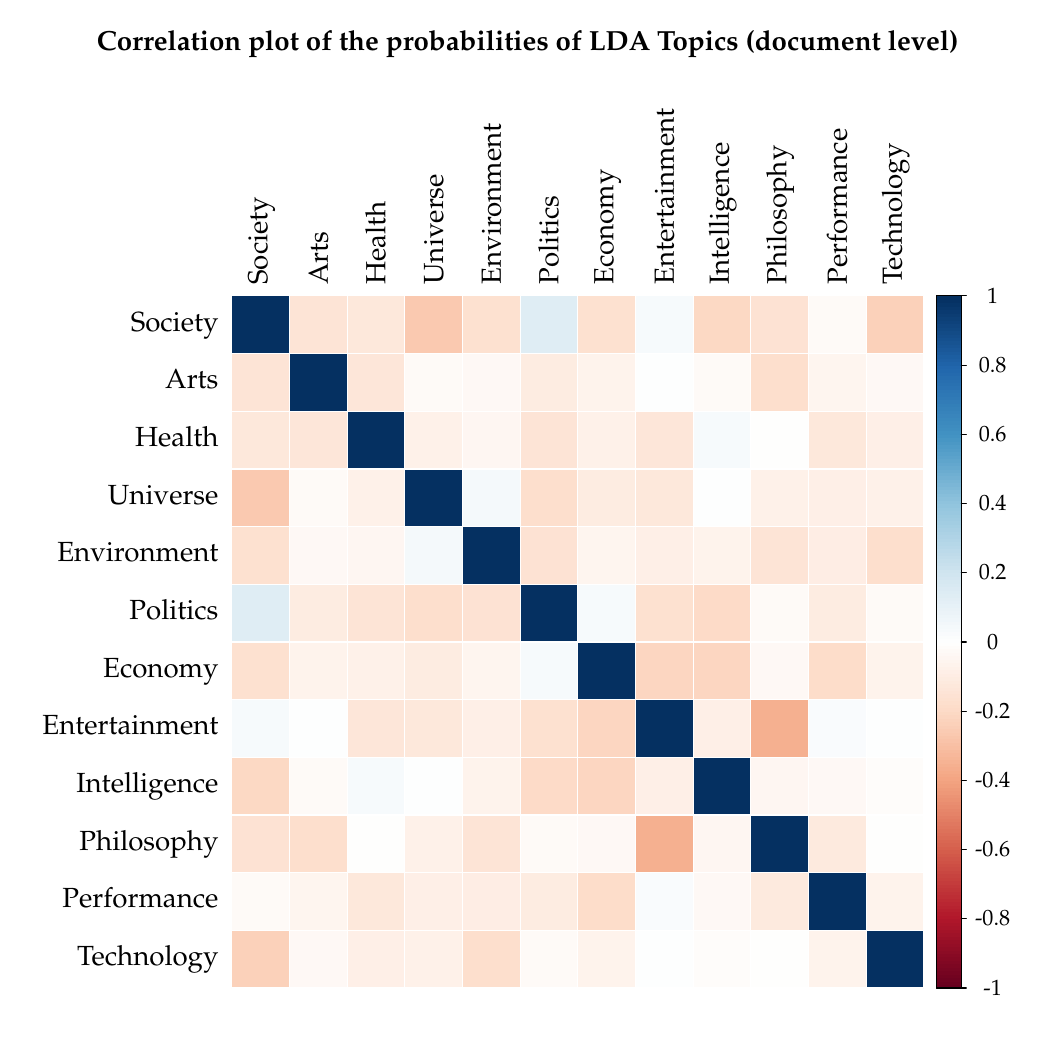
\begin{tikzpicture}[x=1pt,y=1pt]
\definecolor{fillColor}{RGB}{255,255,255}
\path[use as bounding box,fill=fillColor,fill opacity=0.00] (0,0) rectangle (361.35,361.35);
\begin{scope}
\path[clip] (  0.00,  0.00) rectangle (361.35,349.35);
\definecolor{drawColor}{RGB}{255,255,255}
\definecolor{fillColor}{RGB}{255,255,255}

\path[draw=drawColor,line width= 0.4pt,line join=round,line cap=round,fill=fillColor] ( 73.74,243.57) rectangle ( 94.58,264.41);

\path[draw=drawColor,line width= 0.4pt,line join=round,line cap=round,fill=fillColor] ( 73.74,222.73) rectangle ( 94.58,243.57);

\path[draw=drawColor,line width= 0.4pt,line join=round,line cap=round,fill=fillColor] ( 73.74,201.89) rectangle ( 94.58,222.73);

\path[draw=drawColor,line width= 0.4pt,line join=round,line cap=round,fill=fillColor] ( 73.74,181.05) rectangle ( 94.58,201.89);

\path[draw=drawColor,line width= 0.4pt,line join=round,line cap=round,fill=fillColor] ( 73.74,160.21) rectangle ( 94.58,181.05);

\path[draw=drawColor,line width= 0.4pt,line join=round,line cap=round,fill=fillColor] ( 73.74,139.37) rectangle ( 94.58,160.21);

\path[draw=drawColor,line width= 0.4pt,line join=round,line cap=round,fill=fillColor] ( 73.74,118.53) rectangle ( 94.58,139.37);

\path[draw=drawColor,line width= 0.4pt,line join=round,line cap=round,fill=fillColor] ( 73.74, 97.68) rectangle ( 94.58,118.53);

\path[draw=drawColor,line width= 0.4pt,line join=round,line cap=round,fill=fillColor] ( 73.74, 76.84) rectangle ( 94.58, 97.68);

\path[draw=drawColor,line width= 0.4pt,line join=round,line cap=round,fill=fillColor] ( 73.74, 56.00) rectangle ( 94.58, 76.84);

\path[draw=drawColor,line width= 0.4pt,line join=round,line cap=round,fill=fillColor] ( 73.74, 35.16) rectangle ( 94.58, 56.00);

\path[draw=drawColor,line width= 0.4pt,line join=round,line cap=round,fill=fillColor] ( 73.74, 14.32) rectangle ( 94.58, 35.16);

\path[draw=drawColor,line width= 0.4pt,line join=round,line cap=round,fill=fillColor] ( 94.58,243.57) rectangle (115.42,264.41);

\path[draw=drawColor,line width= 0.4pt,line join=round,line cap=round,fill=fillColor] ( 94.58,222.73) rectangle (115.42,243.57);

\path[draw=drawColor,line width= 0.4pt,line join=round,line cap=round,fill=fillColor] ( 94.58,201.89) rectangle (115.42,222.73);

\path[draw=drawColor,line width= 0.4pt,line join=round,line cap=round,fill=fillColor] ( 94.58,181.05) rectangle (115.42,201.89);

\path[draw=drawColor,line width= 0.4pt,line join=round,line cap=round,fill=fillColor] ( 94.58,160.21) rectangle (115.42,181.05);

\path[draw=drawColor,line width= 0.4pt,line join=round,line cap=round,fill=fillColor] ( 94.58,139.37) rectangle (115.42,160.21);

\path[draw=drawColor,line width= 0.4pt,line join=round,line cap=round,fill=fillColor] ( 94.58,118.53) rectangle (115.42,139.37);

\path[draw=drawColor,line width= 0.4pt,line join=round,line cap=round,fill=fillColor] ( 94.58, 97.68) rectangle (115.42,118.53);

\path[draw=drawColor,line width= 0.4pt,line join=round,line cap=round,fill=fillColor] ( 94.58, 76.84) rectangle (115.42, 97.68);

\path[draw=drawColor,line width= 0.4pt,line join=round,line cap=round,fill=fillColor] ( 94.58, 56.00) rectangle (115.42, 76.84);

\path[draw=drawColor,line width= 0.4pt,line join=round,line cap=round,fill=fillColor] ( 94.58, 35.16) rectangle (115.42, 56.00);

\path[draw=drawColor,line width= 0.4pt,line join=round,line cap=round,fill=fillColor] ( 94.58, 14.32) rectangle (115.42, 35.16);

\path[draw=drawColor,line width= 0.4pt,line join=round,line cap=round,fill=fillColor] (115.42,243.57) rectangle (136.27,264.41);

\path[draw=drawColor,line width= 0.4pt,line join=round,line cap=round,fill=fillColor] (115.42,222.73) rectangle (136.27,243.57);

\path[draw=drawColor,line width= 0.4pt,line join=round,line cap=round,fill=fillColor] (115.42,201.89) rectangle (136.27,222.73);

\path[draw=drawColor,line width= 0.4pt,line join=round,line cap=round,fill=fillColor] (115.42,181.05) rectangle (136.27,201.89);

\path[draw=drawColor,line width= 0.4pt,line join=round,line cap=round,fill=fillColor] (115.42,160.21) rectangle (136.27,181.05);

\path[draw=drawColor,line width= 0.4pt,line join=round,line cap=round,fill=fillColor] (115.42,139.37) rectangle (136.27,160.21);

\path[draw=drawColor,line width= 0.4pt,line join=round,line cap=round,fill=fillColor] (115.42,118.53) rectangle (136.27,139.37);

\path[draw=drawColor,line width= 0.4pt,line join=round,line cap=round,fill=fillColor] (115.42, 97.68) rectangle (136.27,118.53);

\path[draw=drawColor,line width= 0.4pt,line join=round,line cap=round,fill=fillColor] (115.42, 76.84) rectangle (136.27, 97.68);

\path[draw=drawColor,line width= 0.4pt,line join=round,line cap=round,fill=fillColor] (115.42, 56.00) rectangle (136.27, 76.84);

\path[draw=drawColor,line width= 0.4pt,line join=round,line cap=round,fill=fillColor] (115.42, 35.16) rectangle (136.27, 56.00);

\path[draw=drawColor,line width= 0.4pt,line join=round,line cap=round,fill=fillColor] (115.42, 14.32) rectangle (136.27, 35.16);

\path[draw=drawColor,line width= 0.4pt,line join=round,line cap=round,fill=fillColor] (136.27,243.57) rectangle (157.11,264.41);

\path[draw=drawColor,line width= 0.4pt,line join=round,line cap=round,fill=fillColor] (136.27,222.73) rectangle (157.11,243.57);

\path[draw=drawColor,line width= 0.4pt,line join=round,line cap=round,fill=fillColor] (136.27,201.89) rectangle (157.11,222.73);

\path[draw=drawColor,line width= 0.4pt,line join=round,line cap=round,fill=fillColor] (136.27,181.05) rectangle (157.11,201.89);

\path[draw=drawColor,line width= 0.4pt,line join=round,line cap=round,fill=fillColor] (136.27,160.21) rectangle (157.11,181.05);

\path[draw=drawColor,line width= 0.4pt,line join=round,line cap=round,fill=fillColor] (136.27,139.37) rectangle (157.11,160.21);

\path[draw=drawColor,line width= 0.4pt,line join=round,line cap=round,fill=fillColor] (136.27,118.53) rectangle (157.11,139.37);

\path[draw=drawColor,line width= 0.4pt,line join=round,line cap=round,fill=fillColor] (136.27, 97.68) rectangle (157.11,118.53);

\path[draw=drawColor,line width= 0.4pt,line join=round,line cap=round,fill=fillColor] (136.27, 76.84) rectangle (157.11, 97.68);

\path[draw=drawColor,line width= 0.4pt,line join=round,line cap=round,fill=fillColor] (136.27, 56.00) rectangle (157.11, 76.84);

\path[draw=drawColor,line width= 0.4pt,line join=round,line cap=round,fill=fillColor] (136.27, 35.16) rectangle (157.11, 56.00);

\path[draw=drawColor,line width= 0.4pt,line join=round,line cap=round,fill=fillColor] (136.27, 14.32) rectangle (157.11, 35.16);

\path[draw=drawColor,line width= 0.4pt,line join=round,line cap=round,fill=fillColor] (157.11,243.57) rectangle (177.95,264.41);

\path[draw=drawColor,line width= 0.4pt,line join=round,line cap=round,fill=fillColor] (157.11,222.73) rectangle (177.95,243.57);

\path[draw=drawColor,line width= 0.4pt,line join=round,line cap=round,fill=fillColor] (157.11,201.89) rectangle (177.95,222.73);

\path[draw=drawColor,line width= 0.4pt,line join=round,line cap=round,fill=fillColor] (157.11,181.05) rectangle (177.95,201.89);

\path[draw=drawColor,line width= 0.4pt,line join=round,line cap=round,fill=fillColor] (157.11,160.21) rectangle (177.95,181.05);

\path[draw=drawColor,line width= 0.4pt,line join=round,line cap=round,fill=fillColor] (157.11,139.37) rectangle (177.95,160.21);

\path[draw=drawColor,line width= 0.4pt,line join=round,line cap=round,fill=fillColor] (157.11,118.53) rectangle (177.95,139.37);

\path[draw=drawColor,line width= 0.4pt,line join=round,line cap=round,fill=fillColor] (157.11, 97.68) rectangle (177.95,118.53);

\path[draw=drawColor,line width= 0.4pt,line join=round,line cap=round,fill=fillColor] (157.11, 76.84) rectangle (177.95, 97.68);

\path[draw=drawColor,line width= 0.4pt,line join=round,line cap=round,fill=fillColor] (157.11, 56.00) rectangle (177.95, 76.84);

\path[draw=drawColor,line width= 0.4pt,line join=round,line cap=round,fill=fillColor] (157.11, 35.16) rectangle (177.95, 56.00);

\path[draw=drawColor,line width= 0.4pt,line join=round,line cap=round,fill=fillColor] (157.11, 14.32) rectangle (177.95, 35.16);

\path[draw=drawColor,line width= 0.4pt,line join=round,line cap=round,fill=fillColor] (177.95,243.57) rectangle (198.79,264.41);

\path[draw=drawColor,line width= 0.4pt,line join=round,line cap=round,fill=fillColor] (177.95,222.73) rectangle (198.79,243.57);

\path[draw=drawColor,line width= 0.4pt,line join=round,line cap=round,fill=fillColor] (177.95,201.89) rectangle (198.79,222.73);

\path[draw=drawColor,line width= 0.4pt,line join=round,line cap=round,fill=fillColor] (177.95,181.05) rectangle (198.79,201.89);

\path[draw=drawColor,line width= 0.4pt,line join=round,line cap=round,fill=fillColor] (177.95,160.21) rectangle (198.79,181.05);

\path[draw=drawColor,line width= 0.4pt,line join=round,line cap=round,fill=fillColor] (177.95,139.37) rectangle (198.79,160.21);

\path[draw=drawColor,line width= 0.4pt,line join=round,line cap=round,fill=fillColor] (177.95,118.53) rectangle (198.79,139.37);

\path[draw=drawColor,line width= 0.4pt,line join=round,line cap=round,fill=fillColor] (177.95, 97.68) rectangle (198.79,118.53);

\path[draw=drawColor,line width= 0.4pt,line join=round,line cap=round,fill=fillColor] (177.95, 76.84) rectangle (198.79, 97.68);

\path[draw=drawColor,line width= 0.4pt,line join=round,line cap=round,fill=fillColor] (177.95, 56.00) rectangle (198.79, 76.84);

\path[draw=drawColor,line width= 0.4pt,line join=round,line cap=round,fill=fillColor] (177.95, 35.16) rectangle (198.79, 56.00);

\path[draw=drawColor,line width= 0.4pt,line join=round,line cap=round,fill=fillColor] (177.95, 14.32) rectangle (198.79, 35.16);

\path[draw=drawColor,line width= 0.4pt,line join=round,line cap=round,fill=fillColor] (198.79,243.57) rectangle (219.63,264.41);

\path[draw=drawColor,line width= 0.4pt,line join=round,line cap=round,fill=fillColor] (198.79,222.73) rectangle (219.63,243.57);

\path[draw=drawColor,line width= 0.4pt,line join=round,line cap=round,fill=fillColor] (198.79,201.89) rectangle (219.63,222.73);

\path[draw=drawColor,line width= 0.4pt,line join=round,line cap=round,fill=fillColor] (198.79,181.05) rectangle (219.63,201.89);

\path[draw=drawColor,line width= 0.4pt,line join=round,line cap=round,fill=fillColor] (198.79,160.21) rectangle (219.63,181.05);

\path[draw=drawColor,line width= 0.4pt,line join=round,line cap=round,fill=fillColor] (198.79,139.37) rectangle (219.63,160.21);

\path[draw=drawColor,line width= 0.4pt,line join=round,line cap=round,fill=fillColor] (198.79,118.53) rectangle (219.63,139.37);

\path[draw=drawColor,line width= 0.4pt,line join=round,line cap=round,fill=fillColor] (198.79, 97.68) rectangle (219.63,118.53);

\path[draw=drawColor,line width= 0.4pt,line join=round,line cap=round,fill=fillColor] (198.79, 76.84) rectangle (219.63, 97.68);

\path[draw=drawColor,line width= 0.4pt,line join=round,line cap=round,fill=fillColor] (198.79, 56.00) rectangle (219.63, 76.84);

\path[draw=drawColor,line width= 0.4pt,line join=round,line cap=round,fill=fillColor] (198.79, 35.16) rectangle (219.63, 56.00);

\path[draw=drawColor,line width= 0.4pt,line join=round,line cap=round,fill=fillColor] (198.79, 14.32) rectangle (219.63, 35.16);

\path[draw=drawColor,line width= 0.4pt,line join=round,line cap=round,fill=fillColor] (219.63,243.57) rectangle (240.47,264.41);

\path[draw=drawColor,line width= 0.4pt,line join=round,line cap=round,fill=fillColor] (219.63,222.73) rectangle (240.47,243.57);

\path[draw=drawColor,line width= 0.4pt,line join=round,line cap=round,fill=fillColor] (219.63,201.89) rectangle (240.47,222.73);

\path[draw=drawColor,line width= 0.4pt,line join=round,line cap=round,fill=fillColor] (219.63,181.05) rectangle (240.47,201.89);

\path[draw=drawColor,line width= 0.4pt,line join=round,line cap=round,fill=fillColor] (219.63,160.21) rectangle (240.47,181.05);

\path[draw=drawColor,line width= 0.4pt,line join=round,line cap=round,fill=fillColor] (219.63,139.37) rectangle (240.47,160.21);

\path[draw=drawColor,line width= 0.4pt,line join=round,line cap=round,fill=fillColor] (219.63,118.53) rectangle (240.47,139.37);

\path[draw=drawColor,line width= 0.4pt,line join=round,line cap=round,fill=fillColor] (219.63, 97.68) rectangle (240.47,118.53);

\path[draw=drawColor,line width= 0.4pt,line join=round,line cap=round,fill=fillColor] (219.63, 76.84) rectangle (240.47, 97.68);

\path[draw=drawColor,line width= 0.4pt,line join=round,line cap=round,fill=fillColor] (219.63, 56.00) rectangle (240.47, 76.84);

\path[draw=drawColor,line width= 0.4pt,line join=round,line cap=round,fill=fillColor] (219.63, 35.16) rectangle (240.47, 56.00);

\path[draw=drawColor,line width= 0.4pt,line join=round,line cap=round,fill=fillColor] (219.63, 14.32) rectangle (240.47, 35.16);

\path[draw=drawColor,line width= 0.4pt,line join=round,line cap=round,fill=fillColor] (240.47,243.57) rectangle (261.31,264.41);

\path[draw=drawColor,line width= 0.4pt,line join=round,line cap=round,fill=fillColor] (240.47,222.73) rectangle (261.31,243.57);

\path[draw=drawColor,line width= 0.4pt,line join=round,line cap=round,fill=fillColor] (240.47,201.89) rectangle (261.31,222.73);

\path[draw=drawColor,line width= 0.4pt,line join=round,line cap=round,fill=fillColor] (240.47,181.05) rectangle (261.31,201.89);

\path[draw=drawColor,line width= 0.4pt,line join=round,line cap=round,fill=fillColor] (240.47,160.21) rectangle (261.31,181.05);

\path[draw=drawColor,line width= 0.4pt,line join=round,line cap=round,fill=fillColor] (240.47,139.37) rectangle (261.31,160.21);

\path[draw=drawColor,line width= 0.4pt,line join=round,line cap=round,fill=fillColor] (240.47,118.53) rectangle (261.31,139.37);

\path[draw=drawColor,line width= 0.4pt,line join=round,line cap=round,fill=fillColor] (240.47, 97.68) rectangle (261.31,118.53);

\path[draw=drawColor,line width= 0.4pt,line join=round,line cap=round,fill=fillColor] (240.47, 76.84) rectangle (261.31, 97.68);

\path[draw=drawColor,line width= 0.4pt,line join=round,line cap=round,fill=fillColor] (240.47, 56.00) rectangle (261.31, 76.84);

\path[draw=drawColor,line width= 0.4pt,line join=round,line cap=round,fill=fillColor] (240.47, 35.16) rectangle (261.31, 56.00);

\path[draw=drawColor,line width= 0.4pt,line join=round,line cap=round,fill=fillColor] (240.47, 14.32) rectangle (261.31, 35.16);

\path[draw=drawColor,line width= 0.4pt,line join=round,line cap=round,fill=fillColor] (261.31,243.57) rectangle (282.15,264.41);

\path[draw=drawColor,line width= 0.4pt,line join=round,line cap=round,fill=fillColor] (261.31,222.73) rectangle (282.15,243.57);

\path[draw=drawColor,line width= 0.4pt,line join=round,line cap=round,fill=fillColor] (261.31,201.89) rectangle (282.15,222.73);

\path[draw=drawColor,line width= 0.4pt,line join=round,line cap=round,fill=fillColor] (261.31,181.05) rectangle (282.15,201.89);

\path[draw=drawColor,line width= 0.4pt,line join=round,line cap=round,fill=fillColor] (261.31,160.21) rectangle (282.15,181.05);

\path[draw=drawColor,line width= 0.4pt,line join=round,line cap=round,fill=fillColor] (261.31,139.37) rectangle (282.15,160.21);

\path[draw=drawColor,line width= 0.4pt,line join=round,line cap=round,fill=fillColor] (261.31,118.53) rectangle (282.15,139.37);

\path[draw=drawColor,line width= 0.4pt,line join=round,line cap=round,fill=fillColor] (261.31, 97.68) rectangle (282.15,118.53);

\path[draw=drawColor,line width= 0.4pt,line join=round,line cap=round,fill=fillColor] (261.31, 76.84) rectangle (282.15, 97.68);

\path[draw=drawColor,line width= 0.4pt,line join=round,line cap=round,fill=fillColor] (261.31, 56.00) rectangle (282.15, 76.84);

\path[draw=drawColor,line width= 0.4pt,line join=round,line cap=round,fill=fillColor] (261.31, 35.16) rectangle (282.15, 56.00);

\path[draw=drawColor,line width= 0.4pt,line join=round,line cap=round,fill=fillColor] (261.31, 14.32) rectangle (282.15, 35.16);

\path[draw=drawColor,line width= 0.4pt,line join=round,line cap=round,fill=fillColor] (282.15,243.57) rectangle (302.99,264.41);

\path[draw=drawColor,line width= 0.4pt,line join=round,line cap=round,fill=fillColor] (282.15,222.73) rectangle (302.99,243.57);

\path[draw=drawColor,line width= 0.4pt,line join=round,line cap=round,fill=fillColor] (282.15,201.89) rectangle (302.99,222.73);

\path[draw=drawColor,line width= 0.4pt,line join=round,line cap=round,fill=fillColor] (282.15,181.05) rectangle (302.99,201.89);

\path[draw=drawColor,line width= 0.4pt,line join=round,line cap=round,fill=fillColor] (282.15,160.21) rectangle (302.99,181.05);

\path[draw=drawColor,line width= 0.4pt,line join=round,line cap=round,fill=fillColor] (282.15,139.37) rectangle (302.99,160.21);

\path[draw=drawColor,line width= 0.4pt,line join=round,line cap=round,fill=fillColor] (282.15,118.53) rectangle (302.99,139.37);

\path[draw=drawColor,line width= 0.4pt,line join=round,line cap=round,fill=fillColor] (282.15, 97.68) rectangle (302.99,118.53);

\path[draw=drawColor,line width= 0.4pt,line join=round,line cap=round,fill=fillColor] (282.15, 76.84) rectangle (302.99, 97.68);

\path[draw=drawColor,line width= 0.4pt,line join=round,line cap=round,fill=fillColor] (282.15, 56.00) rectangle (302.99, 76.84);

\path[draw=drawColor,line width= 0.4pt,line join=round,line cap=round,fill=fillColor] (282.15, 35.16) rectangle (302.99, 56.00);

\path[draw=drawColor,line width= 0.4pt,line join=round,line cap=round,fill=fillColor] (282.15, 14.32) rectangle (302.99, 35.16);

\path[draw=drawColor,line width= 0.4pt,line join=round,line cap=round,fill=fillColor] (302.99,243.57) rectangle (323.84,264.41);

\path[draw=drawColor,line width= 0.4pt,line join=round,line cap=round,fill=fillColor] (302.99,222.73) rectangle (323.84,243.57);

\path[draw=drawColor,line width= 0.4pt,line join=round,line cap=round,fill=fillColor] (302.99,201.89) rectangle (323.84,222.73);

\path[draw=drawColor,line width= 0.4pt,line join=round,line cap=round,fill=fillColor] (302.99,181.05) rectangle (323.84,201.89);

\path[draw=drawColor,line width= 0.4pt,line join=round,line cap=round,fill=fillColor] (302.99,160.21) rectangle (323.84,181.05);

\path[draw=drawColor,line width= 0.4pt,line join=round,line cap=round,fill=fillColor] (302.99,139.37) rectangle (323.84,160.21);

\path[draw=drawColor,line width= 0.4pt,line join=round,line cap=round,fill=fillColor] (302.99,118.53) rectangle (323.84,139.37);

\path[draw=drawColor,line width= 0.4pt,line join=round,line cap=round,fill=fillColor] (302.99, 97.68) rectangle (323.84,118.53);

\path[draw=drawColor,line width= 0.4pt,line join=round,line cap=round,fill=fillColor] (302.99, 76.84) rectangle (323.84, 97.68);

\path[draw=drawColor,line width= 0.4pt,line join=round,line cap=round,fill=fillColor] (302.99, 56.00) rectangle (323.84, 76.84);

\path[draw=drawColor,line width= 0.4pt,line join=round,line cap=round,fill=fillColor] (302.99, 35.16) rectangle (323.84, 56.00);

\path[draw=drawColor,line width= 0.4pt,line join=round,line cap=round,fill=fillColor] (302.99, 14.32) rectangle (323.84, 35.16);
\definecolor{drawColor}{RGB}{5,48,97}
\definecolor{fillColor}{RGB}{5,48,97}

\path[draw=drawColor,line width= 0.4pt,line join=round,line cap=round,fill=fillColor] ( 73.74,243.57) rectangle ( 94.58,264.41);
\definecolor{drawColor}{RGB}{253,228,214}
\definecolor{fillColor}{RGB}{253,228,214}

\path[draw=drawColor,line width= 0.4pt,line join=round,line cap=round,fill=fillColor] ( 73.74,222.73) rectangle ( 94.58,243.57);
\definecolor{drawColor}{RGB}{253,232,219}
\definecolor{fillColor}{RGB}{253,232,219}

\path[draw=drawColor,line width= 0.4pt,line join=round,line cap=round,fill=fillColor] ( 73.74,201.89) rectangle ( 94.58,222.73);
\definecolor{drawColor}{RGB}{250,201,176}
\definecolor{fillColor}{RGB}{250,201,176}

\path[draw=drawColor,line width= 0.4pt,line join=round,line cap=round,fill=fillColor] ( 73.74,181.05) rectangle ( 94.58,201.89);
\definecolor{drawColor}{RGB}{253,225,208}
\definecolor{fillColor}{RGB}{253,225,208}

\path[draw=drawColor,line width= 0.4pt,line join=round,line cap=round,fill=fillColor] ( 73.74,160.21) rectangle ( 94.58,181.05);
\definecolor{drawColor}{RGB}{223,237,244}
\definecolor{fillColor}{RGB}{223,237,244}

\path[draw=drawColor,line width= 0.4pt,line join=round,line cap=round,fill=fillColor] ( 73.74,139.37) rectangle ( 94.58,160.21);
\definecolor{drawColor}{RGB}{253,225,208}
\definecolor{fillColor}{RGB}{253,225,208}

\path[draw=drawColor,line width= 0.4pt,line join=round,line cap=round,fill=fillColor] ( 73.74,118.53) rectangle ( 94.58,139.37);
\definecolor{drawColor}{RGB}{246,250,252}
\definecolor{fillColor}{RGB}{246,250,252}

\path[draw=drawColor,line width= 0.4pt,line join=round,line cap=round,fill=fillColor] ( 73.74, 97.68) rectangle ( 94.58,118.53);
\definecolor{drawColor}{RGB}{252,217,196}
\definecolor{fillColor}{RGB}{252,217,196}

\path[draw=drawColor,line width= 0.4pt,line join=round,line cap=round,fill=fillColor] ( 73.74, 76.84) rectangle ( 94.58, 97.68);
\definecolor{drawColor}{RGB}{253,226,211}
\definecolor{fillColor}{RGB}{253,226,211}

\path[draw=drawColor,line width= 0.4pt,line join=round,line cap=round,fill=fillColor] ( 73.74, 56.00) rectangle ( 94.58, 76.84);
\definecolor{drawColor}{RGB}{254,250,247}
\definecolor{fillColor}{RGB}{254,250,247}

\path[draw=drawColor,line width= 0.4pt,line join=round,line cap=round,fill=fillColor] ( 73.74, 35.16) rectangle ( 94.58, 56.00);
\definecolor{drawColor}{RGB}{251,209,186}
\definecolor{fillColor}{RGB}{251,209,186}

\path[draw=drawColor,line width= 0.4pt,line join=round,line cap=round,fill=fillColor] ( 73.74, 14.32) rectangle ( 94.58, 35.16);
\definecolor{drawColor}{RGB}{253,228,214}
\definecolor{fillColor}{RGB}{253,228,214}

\path[draw=drawColor,line width= 0.4pt,line join=round,line cap=round,fill=fillColor] ( 94.58,243.57) rectangle (115.42,264.41);
\definecolor{drawColor}{RGB}{5,48,97}
\definecolor{fillColor}{RGB}{5,48,97}

\path[draw=drawColor,line width= 0.4pt,line join=round,line cap=round,fill=fillColor] ( 94.58,222.73) rectangle (115.42,243.57);
\definecolor{drawColor}{RGB}{253,230,217}
\definecolor{fillColor}{RGB}{253,230,217}

\path[draw=drawColor,line width= 0.4pt,line join=round,line cap=round,fill=fillColor] ( 94.58,201.89) rectangle (115.42,222.73);
\definecolor{drawColor}{RGB}{254,250,247}
\definecolor{fillColor}{RGB}{254,250,247}

\path[draw=drawColor,line width= 0.4pt,line join=round,line cap=round,fill=fillColor] ( 94.58,181.05) rectangle (115.42,201.89);
\definecolor{drawColor}{RGB}{254,248,245}
\definecolor{fillColor}{RGB}{254,248,245}

\path[draw=drawColor,line width= 0.4pt,line join=round,line cap=round,fill=fillColor] ( 94.58,160.21) rectangle (115.42,181.05);
\definecolor{drawColor}{RGB}{253,236,225}
\definecolor{fillColor}{RGB}{253,236,225}

\path[draw=drawColor,line width= 0.4pt,line join=round,line cap=round,fill=fillColor] ( 94.58,139.37) rectangle (115.42,160.21);
\definecolor{drawColor}{RGB}{254,243,236}
\definecolor{fillColor}{RGB}{254,243,236}

\path[draw=drawColor,line width= 0.4pt,line join=round,line cap=round,fill=fillColor] ( 94.58,118.53) rectangle (115.42,139.37);
\definecolor{drawColor}{RGB}{253,254,254}
\definecolor{fillColor}{RGB}{253,254,254}

\path[draw=drawColor,line width= 0.4pt,line join=round,line cap=round,fill=fillColor] ( 94.58, 97.68) rectangle (115.42,118.53);
\definecolor{drawColor}{RGB}{254,250,247}
\definecolor{fillColor}{RGB}{254,250,247}

\path[draw=drawColor,line width= 0.4pt,line join=round,line cap=round,fill=fillColor] ( 94.58, 76.84) rectangle (115.42, 97.68);
\definecolor{drawColor}{RGB}{253,223,205}
\definecolor{fillColor}{RGB}{253,223,205}

\path[draw=drawColor,line width= 0.4pt,line join=round,line cap=round,fill=fillColor] ( 94.58, 56.00) rectangle (115.42, 76.84);
\definecolor{drawColor}{RGB}{254,245,239}
\definecolor{fillColor}{RGB}{254,245,239}

\path[draw=drawColor,line width= 0.4pt,line join=round,line cap=round,fill=fillColor] ( 94.58, 35.16) rectangle (115.42, 56.00);
\definecolor{drawColor}{RGB}{254,248,245}
\definecolor{fillColor}{RGB}{254,248,245}

\path[draw=drawColor,line width= 0.4pt,line join=round,line cap=round,fill=fillColor] ( 94.58, 14.32) rectangle (115.42, 35.16);
\definecolor{drawColor}{RGB}{253,232,219}
\definecolor{fillColor}{RGB}{253,232,219}

\path[draw=drawColor,line width= 0.4pt,line join=round,line cap=round,fill=fillColor] (115.42,243.57) rectangle (136.27,264.41);
\definecolor{drawColor}{RGB}{253,230,217}
\definecolor{fillColor}{RGB}{253,230,217}

\path[draw=drawColor,line width= 0.4pt,line join=round,line cap=round,fill=fillColor] (115.42,222.73) rectangle (136.27,243.57);
\definecolor{drawColor}{RGB}{5,48,97}
\definecolor{fillColor}{RGB}{5,48,97}

\path[draw=drawColor,line width= 0.4pt,line join=round,line cap=round,fill=fillColor] (115.42,201.89) rectangle (136.27,222.73);
\definecolor{drawColor}{RGB}{254,241,233}
\definecolor{fillColor}{RGB}{254,241,233}

\path[draw=drawColor,line width= 0.4pt,line join=round,line cap=round,fill=fillColor] (115.42,181.05) rectangle (136.27,201.89);
\definecolor{drawColor}{RGB}{254,246,242}
\definecolor{fillColor}{RGB}{254,246,242}

\path[draw=drawColor,line width= 0.4pt,line join=round,line cap=round,fill=fillColor] (115.42,160.21) rectangle (136.27,181.05);
\definecolor{drawColor}{RGB}{253,228,214}
\definecolor{fillColor}{RGB}{253,228,214}

\path[draw=drawColor,line width= 0.4pt,line join=round,line cap=round,fill=fillColor] (115.42,139.37) rectangle (136.27,160.21);
\definecolor{drawColor}{RGB}{254,241,233}
\definecolor{fillColor}{RGB}{254,241,233}

\path[draw=drawColor,line width= 0.4pt,line join=round,line cap=round,fill=fillColor] (115.42,118.53) rectangle (136.27,139.37);
\definecolor{drawColor}{RGB}{253,230,217}
\definecolor{fillColor}{RGB}{253,230,217}

\path[draw=drawColor,line width= 0.4pt,line join=round,line cap=round,fill=fillColor] (115.42, 97.68) rectangle (136.27,118.53);
\definecolor{drawColor}{RGB}{246,250,252}
\definecolor{fillColor}{RGB}{246,250,252}

\path[draw=drawColor,line width= 0.4pt,line join=round,line cap=round,fill=fillColor] (115.42, 76.84) rectangle (136.27, 97.68);
\definecolor{drawColor}{RGB}{254,254,253}
\definecolor{fillColor}{RGB}{254,254,253}

\path[draw=drawColor,line width= 0.4pt,line join=round,line cap=round,fill=fillColor] (115.42, 56.00) rectangle (136.27, 76.84);
\definecolor{drawColor}{RGB}{253,232,219}
\definecolor{fillColor}{RGB}{253,232,219}

\path[draw=drawColor,line width= 0.4pt,line join=round,line cap=round,fill=fillColor] (115.42, 35.16) rectangle (136.27, 56.00);
\definecolor{drawColor}{RGB}{254,239,231}
\definecolor{fillColor}{RGB}{254,239,231}

\path[draw=drawColor,line width= 0.4pt,line join=round,line cap=round,fill=fillColor] (115.42, 14.32) rectangle (136.27, 35.16);
\definecolor{drawColor}{RGB}{250,201,176}
\definecolor{fillColor}{RGB}{250,201,176}

\path[draw=drawColor,line width= 0.4pt,line join=round,line cap=round,fill=fillColor] (136.27,243.57) rectangle (157.11,264.41);
\definecolor{drawColor}{RGB}{254,250,247}
\definecolor{fillColor}{RGB}{254,250,247}

\path[draw=drawColor,line width= 0.4pt,line join=round,line cap=round,fill=fillColor] (136.27,222.73) rectangle (157.11,243.57);
\definecolor{drawColor}{RGB}{254,241,233}
\definecolor{fillColor}{RGB}{254,241,233}

\path[draw=drawColor,line width= 0.4pt,line join=round,line cap=round,fill=fillColor] (136.27,201.89) rectangle (157.11,222.73);
\definecolor{drawColor}{RGB}{5,48,97}
\definecolor{fillColor}{RGB}{5,48,97}

\path[draw=drawColor,line width= 0.4pt,line join=round,line cap=round,fill=fillColor] (136.27,181.05) rectangle (157.11,201.89);
\definecolor{drawColor}{RGB}{244,249,251}
\definecolor{fillColor}{RGB}{244,249,251}

\path[draw=drawColor,line width= 0.4pt,line join=round,line cap=round,fill=fillColor] (136.27,160.21) rectangle (157.11,181.05);
\definecolor{drawColor}{RGB}{253,223,205}
\definecolor{fillColor}{RGB}{253,223,205}

\path[draw=drawColor,line width= 0.4pt,line join=round,line cap=round,fill=fillColor] (136.27,139.37) rectangle (157.11,160.21);
\definecolor{drawColor}{RGB}{253,236,225}
\definecolor{fillColor}{RGB}{253,236,225}

\path[draw=drawColor,line width= 0.4pt,line join=round,line cap=round,fill=fillColor] (136.27,118.53) rectangle (157.11,139.37);
\definecolor{drawColor}{RGB}{253,232,219}
\definecolor{fillColor}{RGB}{253,232,219}

\path[draw=drawColor,line width= 0.4pt,line join=round,line cap=round,fill=fillColor] (136.27, 97.68) rectangle (157.11,118.53);
\definecolor{drawColor}{RGB}{253,254,254}
\definecolor{fillColor}{RGB}{253,254,254}

\path[draw=drawColor,line width= 0.4pt,line join=round,line cap=round,fill=fillColor] (136.27, 76.84) rectangle (157.11, 97.68);
\definecolor{drawColor}{RGB}{254,241,233}
\definecolor{fillColor}{RGB}{254,241,233}

\path[draw=drawColor,line width= 0.4pt,line join=round,line cap=round,fill=fillColor] (136.27, 56.00) rectangle (157.11, 76.84);
\definecolor{drawColor}{RGB}{254,239,231}
\definecolor{fillColor}{RGB}{254,239,231}

\path[draw=drawColor,line width= 0.4pt,line join=round,line cap=round,fill=fillColor] (136.27, 35.16) rectangle (157.11, 56.00);
\definecolor{drawColor}{RGB}{254,241,233}
\definecolor{fillColor}{RGB}{254,241,233}

\path[draw=drawColor,line width= 0.4pt,line join=round,line cap=round,fill=fillColor] (136.27, 14.32) rectangle (157.11, 35.16);
\definecolor{drawColor}{RGB}{253,225,208}
\definecolor{fillColor}{RGB}{253,225,208}

\path[draw=drawColor,line width= 0.4pt,line join=round,line cap=round,fill=fillColor] (157.11,243.57) rectangle (177.95,264.41);
\definecolor{drawColor}{RGB}{254,248,245}
\definecolor{fillColor}{RGB}{254,248,245}

\path[draw=drawColor,line width= 0.4pt,line join=round,line cap=round,fill=fillColor] (157.11,222.73) rectangle (177.95,243.57);
\definecolor{drawColor}{RGB}{254,246,242}
\definecolor{fillColor}{RGB}{254,246,242}

\path[draw=drawColor,line width= 0.4pt,line join=round,line cap=round,fill=fillColor] (157.11,201.89) rectangle (177.95,222.73);
\definecolor{drawColor}{RGB}{244,249,251}
\definecolor{fillColor}{RGB}{244,249,251}

\path[draw=drawColor,line width= 0.4pt,line join=round,line cap=round,fill=fillColor] (157.11,181.05) rectangle (177.95,201.89);
\definecolor{drawColor}{RGB}{5,48,97}
\definecolor{fillColor}{RGB}{5,48,97}

\path[draw=drawColor,line width= 0.4pt,line join=round,line cap=round,fill=fillColor] (157.11,160.21) rectangle (177.95,181.05);
\definecolor{drawColor}{RGB}{253,226,211}
\definecolor{fillColor}{RGB}{253,226,211}

\path[draw=drawColor,line width= 0.4pt,line join=round,line cap=round,fill=fillColor] (157.11,139.37) rectangle (177.95,160.21);
\definecolor{drawColor}{RGB}{254,245,239}
\definecolor{fillColor}{RGB}{254,245,239}

\path[draw=drawColor,line width= 0.4pt,line join=round,line cap=round,fill=fillColor] (157.11,118.53) rectangle (177.95,139.37);
\definecolor{drawColor}{RGB}{254,239,231}
\definecolor{fillColor}{RGB}{254,239,231}

\path[draw=drawColor,line width= 0.4pt,line join=round,line cap=round,fill=fillColor] (157.11, 97.68) rectangle (177.95,118.53);
\definecolor{drawColor}{RGB}{254,243,236}
\definecolor{fillColor}{RGB}{254,243,236}

\path[draw=drawColor,line width= 0.4pt,line join=round,line cap=round,fill=fillColor] (157.11, 76.84) rectangle (177.95, 97.68);
\definecolor{drawColor}{RGB}{253,228,214}
\definecolor{fillColor}{RGB}{253,228,214}

\path[draw=drawColor,line width= 0.4pt,line join=round,line cap=round,fill=fillColor] (157.11, 56.00) rectangle (177.95, 76.84);
\definecolor{drawColor}{RGB}{254,237,228}
\definecolor{fillColor}{RGB}{254,237,228}

\path[draw=drawColor,line width= 0.4pt,line join=round,line cap=round,fill=fillColor] (157.11, 35.16) rectangle (177.95, 56.00);
\definecolor{drawColor}{RGB}{253,223,205}
\definecolor{fillColor}{RGB}{253,223,205}

\path[draw=drawColor,line width= 0.4pt,line join=round,line cap=round,fill=fillColor] (157.11, 14.32) rectangle (177.95, 35.16);
\definecolor{drawColor}{RGB}{223,237,244}
\definecolor{fillColor}{RGB}{223,237,244}

\path[draw=drawColor,line width= 0.4pt,line join=round,line cap=round,fill=fillColor] (177.95,243.57) rectangle (198.79,264.41);
\definecolor{drawColor}{RGB}{253,236,225}
\definecolor{fillColor}{RGB}{253,236,225}

\path[draw=drawColor,line width= 0.4pt,line join=round,line cap=round,fill=fillColor] (177.95,222.73) rectangle (198.79,243.57);
\definecolor{drawColor}{RGB}{253,228,214}
\definecolor{fillColor}{RGB}{253,228,214}

\path[draw=drawColor,line width= 0.4pt,line join=round,line cap=round,fill=fillColor] (177.95,201.89) rectangle (198.79,222.73);
\definecolor{drawColor}{RGB}{253,223,205}
\definecolor{fillColor}{RGB}{253,223,205}

\path[draw=drawColor,line width= 0.4pt,line join=round,line cap=round,fill=fillColor] (177.95,181.05) rectangle (198.79,201.89);
\definecolor{drawColor}{RGB}{253,226,211}
\definecolor{fillColor}{RGB}{253,226,211}

\path[draw=drawColor,line width= 0.4pt,line join=round,line cap=round,fill=fillColor] (177.95,160.21) rectangle (198.79,181.05);
\definecolor{drawColor}{RGB}{5,48,97}
\definecolor{fillColor}{RGB}{5,48,97}

\path[draw=drawColor,line width= 0.4pt,line join=round,line cap=round,fill=fillColor] (177.95,139.37) rectangle (198.79,160.21);
\definecolor{drawColor}{RGB}{246,250,252}
\definecolor{fillColor}{RGB}{246,250,252}

\path[draw=drawColor,line width= 0.4pt,line join=round,line cap=round,fill=fillColor] (177.95,118.53) rectangle (198.79,139.37);
\definecolor{drawColor}{RGB}{253,225,208}
\definecolor{fillColor}{RGB}{253,225,208}

\path[draw=drawColor,line width= 0.4pt,line join=round,line cap=round,fill=fillColor] (177.95, 97.68) rectangle (198.79,118.53);
\definecolor{drawColor}{RGB}{253,219,200}
\definecolor{fillColor}{RGB}{253,219,200}

\path[draw=drawColor,line width= 0.4pt,line join=round,line cap=round,fill=fillColor] (177.95, 76.84) rectangle (198.79, 97.68);
\definecolor{drawColor}{RGB}{254,250,247}
\definecolor{fillColor}{RGB}{254,250,247}

\path[draw=drawColor,line width= 0.4pt,line join=round,line cap=round,fill=fillColor] (177.95, 56.00) rectangle (198.79, 76.84);
\definecolor{drawColor}{RGB}{253,236,225}
\definecolor{fillColor}{RGB}{253,236,225}

\path[draw=drawColor,line width= 0.4pt,line join=round,line cap=round,fill=fillColor] (177.95, 35.16) rectangle (198.79, 56.00);
\definecolor{drawColor}{RGB}{254,250,247}
\definecolor{fillColor}{RGB}{254,250,247}

\path[draw=drawColor,line width= 0.4pt,line join=round,line cap=round,fill=fillColor] (177.95, 14.32) rectangle (198.79, 35.16);
\definecolor{drawColor}{RGB}{253,225,208}
\definecolor{fillColor}{RGB}{253,225,208}

\path[draw=drawColor,line width= 0.4pt,line join=round,line cap=round,fill=fillColor] (198.79,243.57) rectangle (219.63,264.41);
\definecolor{drawColor}{RGB}{254,243,236}
\definecolor{fillColor}{RGB}{254,243,236}

\path[draw=drawColor,line width= 0.4pt,line join=round,line cap=round,fill=fillColor] (198.79,222.73) rectangle (219.63,243.57);
\definecolor{drawColor}{RGB}{254,241,233}
\definecolor{fillColor}{RGB}{254,241,233}

\path[draw=drawColor,line width= 0.4pt,line join=round,line cap=round,fill=fillColor] (198.79,201.89) rectangle (219.63,222.73);
\definecolor{drawColor}{RGB}{253,236,225}
\definecolor{fillColor}{RGB}{253,236,225}

\path[draw=drawColor,line width= 0.4pt,line join=round,line cap=round,fill=fillColor] (198.79,181.05) rectangle (219.63,201.89);
\definecolor{drawColor}{RGB}{254,245,239}
\definecolor{fillColor}{RGB}{254,245,239}

\path[draw=drawColor,line width= 0.4pt,line join=round,line cap=round,fill=fillColor] (198.79,160.21) rectangle (219.63,181.05);
\definecolor{drawColor}{RGB}{246,250,252}
\definecolor{fillColor}{RGB}{246,250,252}

\path[draw=drawColor,line width= 0.4pt,line join=round,line cap=round,fill=fillColor] (198.79,139.37) rectangle (219.63,160.21);
\definecolor{drawColor}{RGB}{5,48,97}
\definecolor{fillColor}{RGB}{5,48,97}

\path[draw=drawColor,line width= 0.4pt,line join=round,line cap=round,fill=fillColor] (198.79,118.53) rectangle (219.63,139.37);
\definecolor{drawColor}{RGB}{252,214,193}
\definecolor{fillColor}{RGB}{252,214,193}

\path[draw=drawColor,line width= 0.4pt,line join=round,line cap=round,fill=fillColor] (198.79, 97.68) rectangle (219.63,118.53);

\path[draw=drawColor,line width= 0.4pt,line join=round,line cap=round,fill=fillColor] (198.79, 76.84) rectangle (219.63, 97.68);
\definecolor{drawColor}{RGB}{254,248,245}
\definecolor{fillColor}{RGB}{254,248,245}

\path[draw=drawColor,line width= 0.4pt,line join=round,line cap=round,fill=fillColor] (198.79, 56.00) rectangle (219.63, 76.84);
\definecolor{drawColor}{RGB}{253,221,202}
\definecolor{fillColor}{RGB}{253,221,202}

\path[draw=drawColor,line width= 0.4pt,line join=round,line cap=round,fill=fillColor] (198.79, 35.16) rectangle (219.63, 56.00);
\definecolor{drawColor}{RGB}{254,243,236}
\definecolor{fillColor}{RGB}{254,243,236}

\path[draw=drawColor,line width= 0.4pt,line join=round,line cap=round,fill=fillColor] (198.79, 14.32) rectangle (219.63, 35.16);
\definecolor{drawColor}{RGB}{246,250,252}
\definecolor{fillColor}{RGB}{246,250,252}

\path[draw=drawColor,line width= 0.4pt,line join=round,line cap=round,fill=fillColor] (219.63,243.57) rectangle (240.47,264.41);
\definecolor{drawColor}{RGB}{253,254,254}
\definecolor{fillColor}{RGB}{253,254,254}

\path[draw=drawColor,line width= 0.4pt,line join=round,line cap=round,fill=fillColor] (219.63,222.73) rectangle (240.47,243.57);
\definecolor{drawColor}{RGB}{253,230,217}
\definecolor{fillColor}{RGB}{253,230,217}

\path[draw=drawColor,line width= 0.4pt,line join=round,line cap=round,fill=fillColor] (219.63,201.89) rectangle (240.47,222.73);
\definecolor{drawColor}{RGB}{253,232,219}
\definecolor{fillColor}{RGB}{253,232,219}

\path[draw=drawColor,line width= 0.4pt,line join=round,line cap=round,fill=fillColor] (219.63,181.05) rectangle (240.47,201.89);
\definecolor{drawColor}{RGB}{254,239,231}
\definecolor{fillColor}{RGB}{254,239,231}

\path[draw=drawColor,line width= 0.4pt,line join=round,line cap=round,fill=fillColor] (219.63,160.21) rectangle (240.47,181.05);
\definecolor{drawColor}{RGB}{253,225,208}
\definecolor{fillColor}{RGB}{253,225,208}

\path[draw=drawColor,line width= 0.4pt,line join=round,line cap=round,fill=fillColor] (219.63,139.37) rectangle (240.47,160.21);
\definecolor{drawColor}{RGB}{252,214,193}
\definecolor{fillColor}{RGB}{252,214,193}

\path[draw=drawColor,line width= 0.4pt,line join=round,line cap=round,fill=fillColor] (219.63,118.53) rectangle (240.47,139.37);
\definecolor{drawColor}{RGB}{5,48,97}
\definecolor{fillColor}{RGB}{5,48,97}

\path[draw=drawColor,line width= 0.4pt,line join=round,line cap=round,fill=fillColor] (219.63, 97.68) rectangle (240.47,118.53);
\definecolor{drawColor}{RGB}{254,239,231}
\definecolor{fillColor}{RGB}{254,239,231}

\path[draw=drawColor,line width= 0.4pt,line join=round,line cap=round,fill=fillColor] (219.63, 76.84) rectangle (240.47, 97.68);
\definecolor{drawColor}{RGB}{245,176,144}
\definecolor{fillColor}{RGB}{245,176,144}

\path[draw=drawColor,line width= 0.4pt,line join=round,line cap=round,fill=fillColor] (219.63, 56.00) rectangle (240.47, 76.84);
\definecolor{drawColor}{RGB}{249,251,253}
\definecolor{fillColor}{RGB}{249,251,253}

\path[draw=drawColor,line width= 0.4pt,line join=round,line cap=round,fill=fillColor] (219.63, 35.16) rectangle (240.47, 56.00);
\definecolor{drawColor}{RGB}{253,254,254}
\definecolor{fillColor}{RGB}{253,254,254}

\path[draw=drawColor,line width= 0.4pt,line join=round,line cap=round,fill=fillColor] (219.63, 14.32) rectangle (240.47, 35.16);
\definecolor{drawColor}{RGB}{252,217,196}
\definecolor{fillColor}{RGB}{252,217,196}

\path[draw=drawColor,line width= 0.4pt,line join=round,line cap=round,fill=fillColor] (240.47,243.57) rectangle (261.31,264.41);
\definecolor{drawColor}{RGB}{254,250,247}
\definecolor{fillColor}{RGB}{254,250,247}

\path[draw=drawColor,line width= 0.4pt,line join=round,line cap=round,fill=fillColor] (240.47,222.73) rectangle (261.31,243.57);
\definecolor{drawColor}{RGB}{246,250,252}
\definecolor{fillColor}{RGB}{246,250,252}

\path[draw=drawColor,line width= 0.4pt,line join=round,line cap=round,fill=fillColor] (240.47,201.89) rectangle (261.31,222.73);
\definecolor{drawColor}{RGB}{253,254,254}
\definecolor{fillColor}{RGB}{253,254,254}

\path[draw=drawColor,line width= 0.4pt,line join=round,line cap=round,fill=fillColor] (240.47,181.05) rectangle (261.31,201.89);
\definecolor{drawColor}{RGB}{254,243,236}
\definecolor{fillColor}{RGB}{254,243,236}

\path[draw=drawColor,line width= 0.4pt,line join=round,line cap=round,fill=fillColor] (240.47,160.21) rectangle (261.31,181.05);
\definecolor{drawColor}{RGB}{253,219,200}
\definecolor{fillColor}{RGB}{253,219,200}

\path[draw=drawColor,line width= 0.4pt,line join=round,line cap=round,fill=fillColor] (240.47,139.37) rectangle (261.31,160.21);
\definecolor{drawColor}{RGB}{252,214,193}
\definecolor{fillColor}{RGB}{252,214,193}

\path[draw=drawColor,line width= 0.4pt,line join=round,line cap=round,fill=fillColor] (240.47,118.53) rectangle (261.31,139.37);
\definecolor{drawColor}{RGB}{254,239,231}
\definecolor{fillColor}{RGB}{254,239,231}

\path[draw=drawColor,line width= 0.4pt,line join=round,line cap=round,fill=fillColor] (240.47, 97.68) rectangle (261.31,118.53);
\definecolor{drawColor}{RGB}{5,48,97}
\definecolor{fillColor}{RGB}{5,48,97}

\path[draw=drawColor,line width= 0.4pt,line join=round,line cap=round,fill=fillColor] (240.47, 76.84) rectangle (261.31, 97.68);
\definecolor{drawColor}{RGB}{254,246,242}
\definecolor{fillColor}{RGB}{254,246,242}

\path[draw=drawColor,line width= 0.4pt,line join=round,line cap=round,fill=fillColor] (240.47, 56.00) rectangle (261.31, 76.84);
\definecolor{drawColor}{RGB}{254,248,245}
\definecolor{fillColor}{RGB}{254,248,245}

\path[draw=drawColor,line width= 0.4pt,line join=round,line cap=round,fill=fillColor] (240.47, 35.16) rectangle (261.31, 56.00);
\definecolor{drawColor}{RGB}{254,252,250}
\definecolor{fillColor}{RGB}{254,252,250}

\path[draw=drawColor,line width= 0.4pt,line join=round,line cap=round,fill=fillColor] (240.47, 14.32) rectangle (261.31, 35.16);
\definecolor{drawColor}{RGB}{253,226,211}
\definecolor{fillColor}{RGB}{253,226,211}

\path[draw=drawColor,line width= 0.4pt,line join=round,line cap=round,fill=fillColor] (261.31,243.57) rectangle (282.15,264.41);
\definecolor{drawColor}{RGB}{253,223,205}
\definecolor{fillColor}{RGB}{253,223,205}

\path[draw=drawColor,line width= 0.4pt,line join=round,line cap=round,fill=fillColor] (261.31,222.73) rectangle (282.15,243.57);
\definecolor{drawColor}{RGB}{254,254,253}
\definecolor{fillColor}{RGB}{254,254,253}

\path[draw=drawColor,line width= 0.4pt,line join=round,line cap=round,fill=fillColor] (261.31,201.89) rectangle (282.15,222.73);
\definecolor{drawColor}{RGB}{254,241,233}
\definecolor{fillColor}{RGB}{254,241,233}

\path[draw=drawColor,line width= 0.4pt,line join=round,line cap=round,fill=fillColor] (261.31,181.05) rectangle (282.15,201.89);
\definecolor{drawColor}{RGB}{253,228,214}
\definecolor{fillColor}{RGB}{253,228,214}

\path[draw=drawColor,line width= 0.4pt,line join=round,line cap=round,fill=fillColor] (261.31,160.21) rectangle (282.15,181.05);
\definecolor{drawColor}{RGB}{254,250,247}
\definecolor{fillColor}{RGB}{254,250,247}

\path[draw=drawColor,line width= 0.4pt,line join=round,line cap=round,fill=fillColor] (261.31,139.37) rectangle (282.15,160.21);
\definecolor{drawColor}{RGB}{254,248,245}
\definecolor{fillColor}{RGB}{254,248,245}

\path[draw=drawColor,line width= 0.4pt,line join=round,line cap=round,fill=fillColor] (261.31,118.53) rectangle (282.15,139.37);
\definecolor{drawColor}{RGB}{245,176,144}
\definecolor{fillColor}{RGB}{245,176,144}

\path[draw=drawColor,line width= 0.4pt,line join=round,line cap=round,fill=fillColor] (261.31, 97.68) rectangle (282.15,118.53);
\definecolor{drawColor}{RGB}{254,246,242}
\definecolor{fillColor}{RGB}{254,246,242}

\path[draw=drawColor,line width= 0.4pt,line join=round,line cap=round,fill=fillColor] (261.31, 76.84) rectangle (282.15, 97.68);
\definecolor{drawColor}{RGB}{5,48,97}
\definecolor{fillColor}{RGB}{5,48,97}

\path[draw=drawColor,line width= 0.4pt,line join=round,line cap=round,fill=fillColor] (261.31, 56.00) rectangle (282.15, 76.84);
\definecolor{drawColor}{RGB}{253,234,222}
\definecolor{fillColor}{RGB}{253,234,222}

\path[draw=drawColor,line width= 0.4pt,line join=round,line cap=round,fill=fillColor] (261.31, 35.16) rectangle (282.15, 56.00);
\definecolor{drawColor}{RGB}{254,254,253}
\definecolor{fillColor}{RGB}{254,254,253}

\path[draw=drawColor,line width= 0.4pt,line join=round,line cap=round,fill=fillColor] (261.31, 14.32) rectangle (282.15, 35.16);
\definecolor{drawColor}{RGB}{254,250,247}
\definecolor{fillColor}{RGB}{254,250,247}

\path[draw=drawColor,line width= 0.4pt,line join=round,line cap=round,fill=fillColor] (282.15,243.57) rectangle (302.99,264.41);
\definecolor{drawColor}{RGB}{254,245,239}
\definecolor{fillColor}{RGB}{254,245,239}

\path[draw=drawColor,line width= 0.4pt,line join=round,line cap=round,fill=fillColor] (282.15,222.73) rectangle (302.99,243.57);
\definecolor{drawColor}{RGB}{253,232,219}
\definecolor{fillColor}{RGB}{253,232,219}

\path[draw=drawColor,line width= 0.4pt,line join=round,line cap=round,fill=fillColor] (282.15,201.89) rectangle (302.99,222.73);
\definecolor{drawColor}{RGB}{254,239,231}
\definecolor{fillColor}{RGB}{254,239,231}

\path[draw=drawColor,line width= 0.4pt,line join=round,line cap=round,fill=fillColor] (282.15,181.05) rectangle (302.99,201.89);
\definecolor{drawColor}{RGB}{254,237,228}
\definecolor{fillColor}{RGB}{254,237,228}

\path[draw=drawColor,line width= 0.4pt,line join=round,line cap=round,fill=fillColor] (282.15,160.21) rectangle (302.99,181.05);
\definecolor{drawColor}{RGB}{253,236,225}
\definecolor{fillColor}{RGB}{253,236,225}

\path[draw=drawColor,line width= 0.4pt,line join=round,line cap=round,fill=fillColor] (282.15,139.37) rectangle (302.99,160.21);
\definecolor{drawColor}{RGB}{253,221,202}
\definecolor{fillColor}{RGB}{253,221,202}

\path[draw=drawColor,line width= 0.4pt,line join=round,line cap=round,fill=fillColor] (282.15,118.53) rectangle (302.99,139.37);
\definecolor{drawColor}{RGB}{249,251,253}
\definecolor{fillColor}{RGB}{249,251,253}

\path[draw=drawColor,line width= 0.4pt,line join=round,line cap=round,fill=fillColor] (282.15, 97.68) rectangle (302.99,118.53);
\definecolor{drawColor}{RGB}{254,248,245}
\definecolor{fillColor}{RGB}{254,248,245}

\path[draw=drawColor,line width= 0.4pt,line join=round,line cap=round,fill=fillColor] (282.15, 76.84) rectangle (302.99, 97.68);
\definecolor{drawColor}{RGB}{253,234,222}
\definecolor{fillColor}{RGB}{253,234,222}

\path[draw=drawColor,line width= 0.4pt,line join=round,line cap=round,fill=fillColor] (282.15, 56.00) rectangle (302.99, 76.84);
\definecolor{drawColor}{RGB}{5,48,97}
\definecolor{fillColor}{RGB}{5,48,97}

\path[draw=drawColor,line width= 0.4pt,line join=round,line cap=round,fill=fillColor] (282.15, 35.16) rectangle (302.99, 56.00);
\definecolor{drawColor}{RGB}{254,243,236}
\definecolor{fillColor}{RGB}{254,243,236}

\path[draw=drawColor,line width= 0.4pt,line join=round,line cap=round,fill=fillColor] (282.15, 14.32) rectangle (302.99, 35.16);
\definecolor{drawColor}{RGB}{251,209,186}
\definecolor{fillColor}{RGB}{251,209,186}

\path[draw=drawColor,line width= 0.4pt,line join=round,line cap=round,fill=fillColor] (302.99,243.57) rectangle (323.84,264.41);
\definecolor{drawColor}{RGB}{254,248,245}
\definecolor{fillColor}{RGB}{254,248,245}

\path[draw=drawColor,line width= 0.4pt,line join=round,line cap=round,fill=fillColor] (302.99,222.73) rectangle (323.84,243.57);
\definecolor{drawColor}{RGB}{254,239,231}
\definecolor{fillColor}{RGB}{254,239,231}

\path[draw=drawColor,line width= 0.4pt,line join=round,line cap=round,fill=fillColor] (302.99,201.89) rectangle (323.84,222.73);
\definecolor{drawColor}{RGB}{254,241,233}
\definecolor{fillColor}{RGB}{254,241,233}

\path[draw=drawColor,line width= 0.4pt,line join=round,line cap=round,fill=fillColor] (302.99,181.05) rectangle (323.84,201.89);
\definecolor{drawColor}{RGB}{253,223,205}
\definecolor{fillColor}{RGB}{253,223,205}

\path[draw=drawColor,line width= 0.4pt,line join=round,line cap=round,fill=fillColor] (302.99,160.21) rectangle (323.84,181.05);
\definecolor{drawColor}{RGB}{254,250,247}
\definecolor{fillColor}{RGB}{254,250,247}

\path[draw=drawColor,line width= 0.4pt,line join=round,line cap=round,fill=fillColor] (302.99,139.37) rectangle (323.84,160.21);
\definecolor{drawColor}{RGB}{254,243,236}
\definecolor{fillColor}{RGB}{254,243,236}

\path[draw=drawColor,line width= 0.4pt,line join=round,line cap=round,fill=fillColor] (302.99,118.53) rectangle (323.84,139.37);
\definecolor{drawColor}{RGB}{253,254,254}
\definecolor{fillColor}{RGB}{253,254,254}

\path[draw=drawColor,line width= 0.4pt,line join=round,line cap=round,fill=fillColor] (302.99, 97.68) rectangle (323.84,118.53);
\definecolor{drawColor}{RGB}{254,252,250}
\definecolor{fillColor}{RGB}{254,252,250}

\path[draw=drawColor,line width= 0.4pt,line join=round,line cap=round,fill=fillColor] (302.99, 76.84) rectangle (323.84, 97.68);
\definecolor{drawColor}{RGB}{254,254,253}
\definecolor{fillColor}{RGB}{254,254,253}

\path[draw=drawColor,line width= 0.4pt,line join=round,line cap=round,fill=fillColor] (302.99, 56.00) rectangle (323.84, 76.84);
\definecolor{drawColor}{RGB}{254,243,236}
\definecolor{fillColor}{RGB}{254,243,236}

\path[draw=drawColor,line width= 0.4pt,line join=round,line cap=round,fill=fillColor] (302.99, 35.16) rectangle (323.84, 56.00);
\definecolor{drawColor}{RGB}{5,48,97}
\definecolor{fillColor}{RGB}{5,48,97}

\path[draw=drawColor,line width= 0.4pt,line join=round,line cap=round,fill=fillColor] (302.99, 14.32) rectangle (323.84, 35.16);
\definecolor{drawColor}{RGB}{255,255,255}

\path[draw=drawColor,line width= 0.4pt,line join=round,line cap=round] ( 73.74,243.57) rectangle ( 94.58,264.41);

\path[draw=drawColor,line width= 0.4pt,line join=round,line cap=round] ( 73.74,222.73) rectangle ( 94.58,243.57);

\path[draw=drawColor,line width= 0.4pt,line join=round,line cap=round] ( 73.74,201.89) rectangle ( 94.58,222.73);

\path[draw=drawColor,line width= 0.4pt,line join=round,line cap=round] ( 73.74,181.05) rectangle ( 94.58,201.89);

\path[draw=drawColor,line width= 0.4pt,line join=round,line cap=round] ( 73.74,160.21) rectangle ( 94.58,181.05);

\path[draw=drawColor,line width= 0.4pt,line join=round,line cap=round] ( 73.74,139.37) rectangle ( 94.58,160.21);

\path[draw=drawColor,line width= 0.4pt,line join=round,line cap=round] ( 73.74,118.53) rectangle ( 94.58,139.37);

\path[draw=drawColor,line width= 0.4pt,line join=round,line cap=round] ( 73.74, 97.68) rectangle ( 94.58,118.53);

\path[draw=drawColor,line width= 0.4pt,line join=round,line cap=round] ( 73.74, 76.84) rectangle ( 94.58, 97.68);

\path[draw=drawColor,line width= 0.4pt,line join=round,line cap=round] ( 73.74, 56.00) rectangle ( 94.58, 76.84);

\path[draw=drawColor,line width= 0.4pt,line join=round,line cap=round] ( 73.74, 35.16) rectangle ( 94.58, 56.00);

\path[draw=drawColor,line width= 0.4pt,line join=round,line cap=round] ( 73.74, 14.32) rectangle ( 94.58, 35.16);

\path[draw=drawColor,line width= 0.4pt,line join=round,line cap=round] ( 94.58,243.57) rectangle (115.42,264.41);

\path[draw=drawColor,line width= 0.4pt,line join=round,line cap=round] ( 94.58,222.73) rectangle (115.42,243.57);

\path[draw=drawColor,line width= 0.4pt,line join=round,line cap=round] ( 94.58,201.89) rectangle (115.42,222.73);

\path[draw=drawColor,line width= 0.4pt,line join=round,line cap=round] ( 94.58,181.05) rectangle (115.42,201.89);

\path[draw=drawColor,line width= 0.4pt,line join=round,line cap=round] ( 94.58,160.21) rectangle (115.42,181.05);

\path[draw=drawColor,line width= 0.4pt,line join=round,line cap=round] ( 94.58,139.37) rectangle (115.42,160.21);

\path[draw=drawColor,line width= 0.4pt,line join=round,line cap=round] ( 94.58,118.53) rectangle (115.42,139.37);

\path[draw=drawColor,line width= 0.4pt,line join=round,line cap=round] ( 94.58, 97.68) rectangle (115.42,118.53);

\path[draw=drawColor,line width= 0.4pt,line join=round,line cap=round] ( 94.58, 76.84) rectangle (115.42, 97.68);

\path[draw=drawColor,line width= 0.4pt,line join=round,line cap=round] ( 94.58, 56.00) rectangle (115.42, 76.84);

\path[draw=drawColor,line width= 0.4pt,line join=round,line cap=round] ( 94.58, 35.16) rectangle (115.42, 56.00);

\path[draw=drawColor,line width= 0.4pt,line join=round,line cap=round] ( 94.58, 14.32) rectangle (115.42, 35.16);

\path[draw=drawColor,line width= 0.4pt,line join=round,line cap=round] (115.42,243.57) rectangle (136.27,264.41);

\path[draw=drawColor,line width= 0.4pt,line join=round,line cap=round] (115.42,222.73) rectangle (136.27,243.57);

\path[draw=drawColor,line width= 0.4pt,line join=round,line cap=round] (115.42,201.89) rectangle (136.27,222.73);

\path[draw=drawColor,line width= 0.4pt,line join=round,line cap=round] (115.42,181.05) rectangle (136.27,201.89);

\path[draw=drawColor,line width= 0.4pt,line join=round,line cap=round] (115.42,160.21) rectangle (136.27,181.05);

\path[draw=drawColor,line width= 0.4pt,line join=round,line cap=round] (115.42,139.37) rectangle (136.27,160.21);

\path[draw=drawColor,line width= 0.4pt,line join=round,line cap=round] (115.42,118.53) rectangle (136.27,139.37);

\path[draw=drawColor,line width= 0.4pt,line join=round,line cap=round] (115.42, 97.68) rectangle (136.27,118.53);

\path[draw=drawColor,line width= 0.4pt,line join=round,line cap=round] (115.42, 76.84) rectangle (136.27, 97.68);

\path[draw=drawColor,line width= 0.4pt,line join=round,line cap=round] (115.42, 56.00) rectangle (136.27, 76.84);

\path[draw=drawColor,line width= 0.4pt,line join=round,line cap=round] (115.42, 35.16) rectangle (136.27, 56.00);

\path[draw=drawColor,line width= 0.4pt,line join=round,line cap=round] (115.42, 14.32) rectangle (136.27, 35.16);

\path[draw=drawColor,line width= 0.4pt,line join=round,line cap=round] (136.27,243.57) rectangle (157.11,264.41);

\path[draw=drawColor,line width= 0.4pt,line join=round,line cap=round] (136.27,222.73) rectangle (157.11,243.57);

\path[draw=drawColor,line width= 0.4pt,line join=round,line cap=round] (136.27,201.89) rectangle (157.11,222.73);

\path[draw=drawColor,line width= 0.4pt,line join=round,line cap=round] (136.27,181.05) rectangle (157.11,201.89);

\path[draw=drawColor,line width= 0.4pt,line join=round,line cap=round] (136.27,160.21) rectangle (157.11,181.05);

\path[draw=drawColor,line width= 0.4pt,line join=round,line cap=round] (136.27,139.37) rectangle (157.11,160.21);

\path[draw=drawColor,line width= 0.4pt,line join=round,line cap=round] (136.27,118.53) rectangle (157.11,139.37);

\path[draw=drawColor,line width= 0.4pt,line join=round,line cap=round] (136.27, 97.68) rectangle (157.11,118.53);

\path[draw=drawColor,line width= 0.4pt,line join=round,line cap=round] (136.27, 76.84) rectangle (157.11, 97.68);

\path[draw=drawColor,line width= 0.4pt,line join=round,line cap=round] (136.27, 56.00) rectangle (157.11, 76.84);

\path[draw=drawColor,line width= 0.4pt,line join=round,line cap=round] (136.27, 35.16) rectangle (157.11, 56.00);

\path[draw=drawColor,line width= 0.4pt,line join=round,line cap=round] (136.27, 14.32) rectangle (157.11, 35.16);

\path[draw=drawColor,line width= 0.4pt,line join=round,line cap=round] (157.11,243.57) rectangle (177.95,264.41);

\path[draw=drawColor,line width= 0.4pt,line join=round,line cap=round] (157.11,222.73) rectangle (177.95,243.57);

\path[draw=drawColor,line width= 0.4pt,line join=round,line cap=round] (157.11,201.89) rectangle (177.95,222.73);

\path[draw=drawColor,line width= 0.4pt,line join=round,line cap=round] (157.11,181.05) rectangle (177.95,201.89);

\path[draw=drawColor,line width= 0.4pt,line join=round,line cap=round] (157.11,160.21) rectangle (177.95,181.05);

\path[draw=drawColor,line width= 0.4pt,line join=round,line cap=round] (157.11,139.37) rectangle (177.95,160.21);

\path[draw=drawColor,line width= 0.4pt,line join=round,line cap=round] (157.11,118.53) rectangle (177.95,139.37);

\path[draw=drawColor,line width= 0.4pt,line join=round,line cap=round] (157.11, 97.68) rectangle (177.95,118.53);

\path[draw=drawColor,line width= 0.4pt,line join=round,line cap=round] (157.11, 76.84) rectangle (177.95, 97.68);

\path[draw=drawColor,line width= 0.4pt,line join=round,line cap=round] (157.11, 56.00) rectangle (177.95, 76.84);

\path[draw=drawColor,line width= 0.4pt,line join=round,line cap=round] (157.11, 35.16) rectangle (177.95, 56.00);

\path[draw=drawColor,line width= 0.4pt,line join=round,line cap=round] (157.11, 14.32) rectangle (177.95, 35.16);

\path[draw=drawColor,line width= 0.4pt,line join=round,line cap=round] (177.95,243.57) rectangle (198.79,264.41);

\path[draw=drawColor,line width= 0.4pt,line join=round,line cap=round] (177.95,222.73) rectangle (198.79,243.57);

\path[draw=drawColor,line width= 0.4pt,line join=round,line cap=round] (177.95,201.89) rectangle (198.79,222.73);

\path[draw=drawColor,line width= 0.4pt,line join=round,line cap=round] (177.95,181.05) rectangle (198.79,201.89);

\path[draw=drawColor,line width= 0.4pt,line join=round,line cap=round] (177.95,160.21) rectangle (198.79,181.05);

\path[draw=drawColor,line width= 0.4pt,line join=round,line cap=round] (177.95,139.37) rectangle (198.79,160.21);

\path[draw=drawColor,line width= 0.4pt,line join=round,line cap=round] (177.95,118.53) rectangle (198.79,139.37);

\path[draw=drawColor,line width= 0.4pt,line join=round,line cap=round] (177.95, 97.68) rectangle (198.79,118.53);

\path[draw=drawColor,line width= 0.4pt,line join=round,line cap=round] (177.95, 76.84) rectangle (198.79, 97.68);

\path[draw=drawColor,line width= 0.4pt,line join=round,line cap=round] (177.95, 56.00) rectangle (198.79, 76.84);

\path[draw=drawColor,line width= 0.4pt,line join=round,line cap=round] (177.95, 35.16) rectangle (198.79, 56.00);

\path[draw=drawColor,line width= 0.4pt,line join=round,line cap=round] (177.95, 14.32) rectangle (198.79, 35.16);

\path[draw=drawColor,line width= 0.4pt,line join=round,line cap=round] (198.79,243.57) rectangle (219.63,264.41);

\path[draw=drawColor,line width= 0.4pt,line join=round,line cap=round] (198.79,222.73) rectangle (219.63,243.57);

\path[draw=drawColor,line width= 0.4pt,line join=round,line cap=round] (198.79,201.89) rectangle (219.63,222.73);

\path[draw=drawColor,line width= 0.4pt,line join=round,line cap=round] (198.79,181.05) rectangle (219.63,201.89);

\path[draw=drawColor,line width= 0.4pt,line join=round,line cap=round] (198.79,160.21) rectangle (219.63,181.05);

\path[draw=drawColor,line width= 0.4pt,line join=round,line cap=round] (198.79,139.37) rectangle (219.63,160.21);

\path[draw=drawColor,line width= 0.4pt,line join=round,line cap=round] (198.79,118.53) rectangle (219.63,139.37);

\path[draw=drawColor,line width= 0.4pt,line join=round,line cap=round] (198.79, 97.68) rectangle (219.63,118.53);

\path[draw=drawColor,line width= 0.4pt,line join=round,line cap=round] (198.79, 76.84) rectangle (219.63, 97.68);

\path[draw=drawColor,line width= 0.4pt,line join=round,line cap=round] (198.79, 56.00) rectangle (219.63, 76.84);

\path[draw=drawColor,line width= 0.4pt,line join=round,line cap=round] (198.79, 35.16) rectangle (219.63, 56.00);

\path[draw=drawColor,line width= 0.4pt,line join=round,line cap=round] (198.79, 14.32) rectangle (219.63, 35.16);

\path[draw=drawColor,line width= 0.4pt,line join=round,line cap=round] (219.63,243.57) rectangle (240.47,264.41);

\path[draw=drawColor,line width= 0.4pt,line join=round,line cap=round] (219.63,222.73) rectangle (240.47,243.57);

\path[draw=drawColor,line width= 0.4pt,line join=round,line cap=round] (219.63,201.89) rectangle (240.47,222.73);

\path[draw=drawColor,line width= 0.4pt,line join=round,line cap=round] (219.63,181.05) rectangle (240.47,201.89);

\path[draw=drawColor,line width= 0.4pt,line join=round,line cap=round] (219.63,160.21) rectangle (240.47,181.05);

\path[draw=drawColor,line width= 0.4pt,line join=round,line cap=round] (219.63,139.37) rectangle (240.47,160.21);

\path[draw=drawColor,line width= 0.4pt,line join=round,line cap=round] (219.63,118.53) rectangle (240.47,139.37);

\path[draw=drawColor,line width= 0.4pt,line join=round,line cap=round] (219.63, 97.68) rectangle (240.47,118.53);

\path[draw=drawColor,line width= 0.4pt,line join=round,line cap=round] (219.63, 76.84) rectangle (240.47, 97.68);

\path[draw=drawColor,line width= 0.4pt,line join=round,line cap=round] (219.63, 56.00) rectangle (240.47, 76.84);

\path[draw=drawColor,line width= 0.4pt,line join=round,line cap=round] (219.63, 35.16) rectangle (240.47, 56.00);

\path[draw=drawColor,line width= 0.4pt,line join=round,line cap=round] (219.63, 14.32) rectangle (240.47, 35.16);

\path[draw=drawColor,line width= 0.4pt,line join=round,line cap=round] (240.47,243.57) rectangle (261.31,264.41);

\path[draw=drawColor,line width= 0.4pt,line join=round,line cap=round] (240.47,222.73) rectangle (261.31,243.57);

\path[draw=drawColor,line width= 0.4pt,line join=round,line cap=round] (240.47,201.89) rectangle (261.31,222.73);

\path[draw=drawColor,line width= 0.4pt,line join=round,line cap=round] (240.47,181.05) rectangle (261.31,201.89);

\path[draw=drawColor,line width= 0.4pt,line join=round,line cap=round] (240.47,160.21) rectangle (261.31,181.05);

\path[draw=drawColor,line width= 0.4pt,line join=round,line cap=round] (240.47,139.37) rectangle (261.31,160.21);

\path[draw=drawColor,line width= 0.4pt,line join=round,line cap=round] (240.47,118.53) rectangle (261.31,139.37);

\path[draw=drawColor,line width= 0.4pt,line join=round,line cap=round] (240.47, 97.68) rectangle (261.31,118.53);

\path[draw=drawColor,line width= 0.4pt,line join=round,line cap=round] (240.47, 76.84) rectangle (261.31, 97.68);

\path[draw=drawColor,line width= 0.4pt,line join=round,line cap=round] (240.47, 56.00) rectangle (261.31, 76.84);

\path[draw=drawColor,line width= 0.4pt,line join=round,line cap=round] (240.47, 35.16) rectangle (261.31, 56.00);

\path[draw=drawColor,line width= 0.4pt,line join=round,line cap=round] (240.47, 14.32) rectangle (261.31, 35.16);

\path[draw=drawColor,line width= 0.4pt,line join=round,line cap=round] (261.31,243.57) rectangle (282.15,264.41);

\path[draw=drawColor,line width= 0.4pt,line join=round,line cap=round] (261.31,222.73) rectangle (282.15,243.57);

\path[draw=drawColor,line width= 0.4pt,line join=round,line cap=round] (261.31,201.89) rectangle (282.15,222.73);

\path[draw=drawColor,line width= 0.4pt,line join=round,line cap=round] (261.31,181.05) rectangle (282.15,201.89);

\path[draw=drawColor,line width= 0.4pt,line join=round,line cap=round] (261.31,160.21) rectangle (282.15,181.05);

\path[draw=drawColor,line width= 0.4pt,line join=round,line cap=round] (261.31,139.37) rectangle (282.15,160.21);

\path[draw=drawColor,line width= 0.4pt,line join=round,line cap=round] (261.31,118.53) rectangle (282.15,139.37);

\path[draw=drawColor,line width= 0.4pt,line join=round,line cap=round] (261.31, 97.68) rectangle (282.15,118.53);

\path[draw=drawColor,line width= 0.4pt,line join=round,line cap=round] (261.31, 76.84) rectangle (282.15, 97.68);

\path[draw=drawColor,line width= 0.4pt,line join=round,line cap=round] (261.31, 56.00) rectangle (282.15, 76.84);

\path[draw=drawColor,line width= 0.4pt,line join=round,line cap=round] (261.31, 35.16) rectangle (282.15, 56.00);

\path[draw=drawColor,line width= 0.4pt,line join=round,line cap=round] (261.31, 14.32) rectangle (282.15, 35.16);

\path[draw=drawColor,line width= 0.4pt,line join=round,line cap=round] (282.15,243.57) rectangle (302.99,264.41);

\path[draw=drawColor,line width= 0.4pt,line join=round,line cap=round] (282.15,222.73) rectangle (302.99,243.57);

\path[draw=drawColor,line width= 0.4pt,line join=round,line cap=round] (282.15,201.89) rectangle (302.99,222.73);

\path[draw=drawColor,line width= 0.4pt,line join=round,line cap=round] (282.15,181.05) rectangle (302.99,201.89);

\path[draw=drawColor,line width= 0.4pt,line join=round,line cap=round] (282.15,160.21) rectangle (302.99,181.05);

\path[draw=drawColor,line width= 0.4pt,line join=round,line cap=round] (282.15,139.37) rectangle (302.99,160.21);

\path[draw=drawColor,line width= 0.4pt,line join=round,line cap=round] (282.15,118.53) rectangle (302.99,139.37);

\path[draw=drawColor,line width= 0.4pt,line join=round,line cap=round] (282.15, 97.68) rectangle (302.99,118.53);

\path[draw=drawColor,line width= 0.4pt,line join=round,line cap=round] (282.15, 76.84) rectangle (302.99, 97.68);

\path[draw=drawColor,line width= 0.4pt,line join=round,line cap=round] (282.15, 56.00) rectangle (302.99, 76.84);

\path[draw=drawColor,line width= 0.4pt,line join=round,line cap=round] (282.15, 35.16) rectangle (302.99, 56.00);

\path[draw=drawColor,line width= 0.4pt,line join=round,line cap=round] (282.15, 14.32) rectangle (302.99, 35.16);

\path[draw=drawColor,line width= 0.4pt,line join=round,line cap=round] (302.99,243.57) rectangle (323.84,264.41);

\path[draw=drawColor,line width= 0.4pt,line join=round,line cap=round] (302.99,222.73) rectangle (323.84,243.57);

\path[draw=drawColor,line width= 0.4pt,line join=round,line cap=round] (302.99,201.89) rectangle (323.84,222.73);

\path[draw=drawColor,line width= 0.4pt,line join=round,line cap=round] (302.99,181.05) rectangle (323.84,201.89);

\path[draw=drawColor,line width= 0.4pt,line join=round,line cap=round] (302.99,160.21) rectangle (323.84,181.05);

\path[draw=drawColor,line width= 0.4pt,line join=round,line cap=round] (302.99,139.37) rectangle (323.84,160.21);

\path[draw=drawColor,line width= 0.4pt,line join=round,line cap=round] (302.99,118.53) rectangle (323.84,139.37);

\path[draw=drawColor,line width= 0.4pt,line join=round,line cap=round] (302.99, 97.68) rectangle (323.84,118.53);

\path[draw=drawColor,line width= 0.4pt,line join=round,line cap=round] (302.99, 76.84) rectangle (323.84, 97.68);

\path[draw=drawColor,line width= 0.4pt,line join=round,line cap=round] (302.99, 56.00) rectangle (323.84, 76.84);

\path[draw=drawColor,line width= 0.4pt,line join=round,line cap=round] (302.99, 35.16) rectangle (323.84, 56.00);

\path[draw=drawColor,line width= 0.4pt,line join=round,line cap=round] (302.99, 14.32) rectangle (323.84, 35.16);
\definecolor{drawColor}{RGB}{103,0,31}
\definecolor{fillColor}{RGB}{103,0,31}

\path[draw=drawColor,line width= 0.4pt,line join=round,line cap=round,fill=fillColor] (328.42, 14.32) rectangle (337.36, 15.57);
\definecolor{drawColor}{RGB}{106,1,31}
\definecolor{fillColor}{RGB}{106,1,31}

\path[draw=drawColor,line width= 0.4pt,line join=round,line cap=round,fill=fillColor] (328.42, 15.57) rectangle (337.36, 16.82);
\definecolor{drawColor}{RGB}{110,2,32}
\definecolor{fillColor}{RGB}{110,2,32}

\path[draw=drawColor,line width= 0.4pt,line join=round,line cap=round,fill=fillColor] (328.42, 16.82) rectangle (337.36, 18.07);
\definecolor{drawColor}{RGB}{114,3,32}
\definecolor{fillColor}{RGB}{114,3,32}

\path[draw=drawColor,line width= 0.4pt,line join=round,line cap=round,fill=fillColor] (328.42, 18.07) rectangle (337.36, 19.32);
\definecolor{drawColor}{RGB}{118,4,33}
\definecolor{fillColor}{RGB}{118,4,33}

\path[draw=drawColor,line width= 0.4pt,line join=round,line cap=round,fill=fillColor] (328.42, 19.32) rectangle (337.36, 20.57);
\definecolor{drawColor}{RGB}{121,6,34}
\definecolor{fillColor}{RGB}{121,6,34}

\path[draw=drawColor,line width= 0.4pt,line join=round,line cap=round,fill=fillColor] (328.42, 20.57) rectangle (337.36, 21.82);
\definecolor{drawColor}{RGB}{125,7,34}
\definecolor{fillColor}{RGB}{125,7,34}

\path[draw=drawColor,line width= 0.4pt,line join=round,line cap=round,fill=fillColor] (328.42, 21.82) rectangle (337.36, 23.07);
\definecolor{drawColor}{RGB}{129,8,35}
\definecolor{fillColor}{RGB}{129,8,35}

\path[draw=drawColor,line width= 0.4pt,line join=round,line cap=round,fill=fillColor] (328.42, 23.07) rectangle (337.36, 24.32);
\definecolor{drawColor}{RGB}{133,9,35}
\definecolor{fillColor}{RGB}{133,9,35}

\path[draw=drawColor,line width= 0.4pt,line join=round,line cap=round,fill=fillColor] (328.42, 24.32) rectangle (337.36, 25.57);
\definecolor{drawColor}{RGB}{136,10,36}
\definecolor{fillColor}{RGB}{136,10,36}

\path[draw=drawColor,line width= 0.4pt,line join=round,line cap=round,fill=fillColor] (328.42, 25.57) rectangle (337.36, 26.82);
\definecolor{drawColor}{RGB}{140,12,37}
\definecolor{fillColor}{RGB}{140,12,37}

\path[draw=drawColor,line width= 0.4pt,line join=round,line cap=round,fill=fillColor] (328.42, 26.82) rectangle (337.36, 28.08);
\definecolor{drawColor}{RGB}{144,13,37}
\definecolor{fillColor}{RGB}{144,13,37}

\path[draw=drawColor,line width= 0.4pt,line join=round,line cap=round,fill=fillColor] (328.42, 28.08) rectangle (337.36, 29.33);
\definecolor{drawColor}{RGB}{148,14,38}
\definecolor{fillColor}{RGB}{148,14,38}

\path[draw=drawColor,line width= 0.4pt,line join=round,line cap=round,fill=fillColor] (328.42, 29.33) rectangle (337.36, 30.58);
\definecolor{drawColor}{RGB}{151,15,38}
\definecolor{fillColor}{RGB}{151,15,38}

\path[draw=drawColor,line width= 0.4pt,line join=round,line cap=round,fill=fillColor] (328.42, 30.58) rectangle (337.36, 31.83);
\definecolor{drawColor}{RGB}{155,16,39}
\definecolor{fillColor}{RGB}{155,16,39}

\path[draw=drawColor,line width= 0.4pt,line join=round,line cap=round,fill=fillColor] (328.42, 31.83) rectangle (337.36, 33.08);
\definecolor{drawColor}{RGB}{159,18,40}
\definecolor{fillColor}{RGB}{159,18,40}

\path[draw=drawColor,line width= 0.4pt,line join=round,line cap=round,fill=fillColor] (328.42, 33.08) rectangle (337.36, 34.33);
\definecolor{drawColor}{RGB}{163,19,40}
\definecolor{fillColor}{RGB}{163,19,40}

\path[draw=drawColor,line width= 0.4pt,line join=round,line cap=round,fill=fillColor] (328.42, 34.33) rectangle (337.36, 35.58);
\definecolor{drawColor}{RGB}{167,20,41}
\definecolor{fillColor}{RGB}{167,20,41}

\path[draw=drawColor,line width= 0.4pt,line join=round,line cap=round,fill=fillColor] (328.42, 35.58) rectangle (337.36, 36.83);
\definecolor{drawColor}{RGB}{170,21,41}
\definecolor{fillColor}{RGB}{170,21,41}

\path[draw=drawColor,line width= 0.4pt,line join=round,line cap=round,fill=fillColor] (328.42, 36.83) rectangle (337.36, 38.08);
\definecolor{drawColor}{RGB}{174,22,42}
\definecolor{fillColor}{RGB}{174,22,42}

\path[draw=drawColor,line width= 0.4pt,line join=round,line cap=round,fill=fillColor] (328.42, 38.08) rectangle (337.36, 39.33);
\definecolor{drawColor}{RGB}{178,24,43}
\definecolor{fillColor}{RGB}{178,24,43}

\path[draw=drawColor,line width= 0.4pt,line join=round,line cap=round,fill=fillColor] (328.42, 39.33) rectangle (337.36, 40.58);
\definecolor{drawColor}{RGB}{179,27,44}
\definecolor{fillColor}{RGB}{179,27,44}

\path[draw=drawColor,line width= 0.4pt,line join=round,line cap=round,fill=fillColor] (328.42, 40.58) rectangle (337.36, 41.83);
\definecolor{drawColor}{RGB}{181,31,46}
\definecolor{fillColor}{RGB}{181,31,46}

\path[draw=drawColor,line width= 0.4pt,line join=round,line cap=round,fill=fillColor] (328.42, 41.83) rectangle (337.36, 43.08);
\definecolor{drawColor}{RGB}{183,35,48}
\definecolor{fillColor}{RGB}{183,35,48}

\path[draw=drawColor,line width= 0.4pt,line join=round,line cap=round,fill=fillColor] (328.42, 43.08) rectangle (337.36, 44.33);
\definecolor{drawColor}{RGB}{185,38,50}
\definecolor{fillColor}{RGB}{185,38,50}

\path[draw=drawColor,line width= 0.4pt,line join=round,line cap=round,fill=fillColor] (328.42, 44.33) rectangle (337.36, 45.58);
\definecolor{drawColor}{RGB}{187,42,51}
\definecolor{fillColor}{RGB}{187,42,51}

\path[draw=drawColor,line width= 0.4pt,line join=round,line cap=round,fill=fillColor] (328.42, 45.58) rectangle (337.36, 46.83);
\definecolor{drawColor}{RGB}{189,46,53}
\definecolor{fillColor}{RGB}{189,46,53}

\path[draw=drawColor,line width= 0.4pt,line join=round,line cap=round,fill=fillColor] (328.42, 46.83) rectangle (337.36, 48.08);
\definecolor{drawColor}{RGB}{190,49,55}
\definecolor{fillColor}{RGB}{190,49,55}

\path[draw=drawColor,line width= 0.4pt,line join=round,line cap=round,fill=fillColor] (328.42, 48.08) rectangle (337.36, 49.33);
\definecolor{drawColor}{RGB}{192,53,56}
\definecolor{fillColor}{RGB}{192,53,56}

\path[draw=drawColor,line width= 0.4pt,line join=round,line cap=round,fill=fillColor] (328.42, 49.33) rectangle (337.36, 50.58);
\definecolor{drawColor}{RGB}{194,56,58}
\definecolor{fillColor}{RGB}{194,56,58}

\path[draw=drawColor,line width= 0.4pt,line join=round,line cap=round,fill=fillColor] (328.42, 50.58) rectangle (337.36, 51.83);
\definecolor{drawColor}{RGB}{196,60,60}
\definecolor{fillColor}{RGB}{196,60,60}

\path[draw=drawColor,line width= 0.4pt,line join=round,line cap=round,fill=fillColor] (328.42, 51.83) rectangle (337.36, 53.08);
\definecolor{drawColor}{RGB}{198,64,61}
\definecolor{fillColor}{RGB}{198,64,61}

\path[draw=drawColor,line width= 0.4pt,line join=round,line cap=round,fill=fillColor] (328.42, 53.08) rectangle (337.36, 54.34);
\definecolor{drawColor}{RGB}{199,67,63}
\definecolor{fillColor}{RGB}{199,67,63}

\path[draw=drawColor,line width= 0.4pt,line join=round,line cap=round,fill=fillColor] (328.42, 54.34) rectangle (337.36, 55.59);
\definecolor{drawColor}{RGB}{201,71,65}
\definecolor{fillColor}{RGB}{201,71,65}

\path[draw=drawColor,line width= 0.4pt,line join=round,line cap=round,fill=fillColor] (328.42, 55.59) rectangle (337.36, 56.84);
\definecolor{drawColor}{RGB}{203,75,67}
\definecolor{fillColor}{RGB}{203,75,67}

\path[draw=drawColor,line width= 0.4pt,line join=round,line cap=round,fill=fillColor] (328.42, 56.84) rectangle (337.36, 58.09);
\definecolor{drawColor}{RGB}{205,78,68}
\definecolor{fillColor}{RGB}{205,78,68}

\path[draw=drawColor,line width= 0.4pt,line join=round,line cap=round,fill=fillColor] (328.42, 58.09) rectangle (337.36, 59.34);
\definecolor{drawColor}{RGB}{207,82,70}
\definecolor{fillColor}{RGB}{207,82,70}

\path[draw=drawColor,line width= 0.4pt,line join=round,line cap=round,fill=fillColor] (328.42, 59.34) rectangle (337.36, 60.59);
\definecolor{drawColor}{RGB}{208,85,72}
\definecolor{fillColor}{RGB}{208,85,72}

\path[draw=drawColor,line width= 0.4pt,line join=round,line cap=round,fill=fillColor] (328.42, 60.59) rectangle (337.36, 61.84);
\definecolor{drawColor}{RGB}{210,89,73}
\definecolor{fillColor}{RGB}{210,89,73}

\path[draw=drawColor,line width= 0.4pt,line join=round,line cap=round,fill=fillColor] (328.42, 61.84) rectangle (337.36, 63.09);
\definecolor{drawColor}{RGB}{212,93,75}
\definecolor{fillColor}{RGB}{212,93,75}

\path[draw=drawColor,line width= 0.4pt,line join=round,line cap=round,fill=fillColor] (328.42, 63.09) rectangle (337.36, 64.34);
\definecolor{drawColor}{RGB}{214,96,77}
\definecolor{fillColor}{RGB}{214,96,77}

\path[draw=drawColor,line width= 0.4pt,line join=round,line cap=round,fill=fillColor] (328.42, 64.34) rectangle (337.36, 65.59);
\definecolor{drawColor}{RGB}{215,100,80}
\definecolor{fillColor}{RGB}{215,100,80}

\path[draw=drawColor,line width= 0.4pt,line join=round,line cap=round,fill=fillColor] (328.42, 65.59) rectangle (337.36, 66.84);
\definecolor{drawColor}{RGB}{217,103,82}
\definecolor{fillColor}{RGB}{217,103,82}

\path[draw=drawColor,line width= 0.4pt,line join=round,line cap=round,fill=fillColor] (328.42, 66.84) rectangle (337.36, 68.09);
\definecolor{drawColor}{RGB}{218,107,85}
\definecolor{fillColor}{RGB}{218,107,85}

\path[draw=drawColor,line width= 0.4pt,line join=round,line cap=round,fill=fillColor] (328.42, 68.09) rectangle (337.36, 69.34);
\definecolor{drawColor}{RGB}{220,110,88}
\definecolor{fillColor}{RGB}{220,110,88}

\path[draw=drawColor,line width= 0.4pt,line join=round,line cap=round,fill=fillColor] (328.42, 69.34) rectangle (337.36, 70.59);
\definecolor{drawColor}{RGB}{221,114,90}
\definecolor{fillColor}{RGB}{221,114,90}

\path[draw=drawColor,line width= 0.4pt,line join=round,line cap=round,fill=fillColor] (328.42, 70.59) rectangle (337.36, 71.84);
\definecolor{drawColor}{RGB}{223,117,93}
\definecolor{fillColor}{RGB}{223,117,93}

\path[draw=drawColor,line width= 0.4pt,line join=round,line cap=round,fill=fillColor] (328.42, 71.84) rectangle (337.36, 73.09);
\definecolor{drawColor}{RGB}{224,120,96}
\definecolor{fillColor}{RGB}{224,120,96}

\path[draw=drawColor,line width= 0.4pt,line join=round,line cap=round,fill=fillColor] (328.42, 73.09) rectangle (337.36, 74.34);
\definecolor{drawColor}{RGB}{226,124,98}
\definecolor{fillColor}{RGB}{226,124,98}

\path[draw=drawColor,line width= 0.4pt,line join=round,line cap=round,fill=fillColor] (328.42, 74.34) rectangle (337.36, 75.59);
\definecolor{drawColor}{RGB}{227,127,101}
\definecolor{fillColor}{RGB}{227,127,101}

\path[draw=drawColor,line width= 0.4pt,line join=round,line cap=round,fill=fillColor] (328.42, 75.59) rectangle (337.36, 76.84);
\definecolor{drawColor}{RGB}{229,131,104}
\definecolor{fillColor}{RGB}{229,131,104}

\path[draw=drawColor,line width= 0.4pt,line join=round,line cap=round,fill=fillColor] (328.42, 76.84) rectangle (337.36, 78.09);
\definecolor{drawColor}{RGB}{230,134,106}
\definecolor{fillColor}{RGB}{230,134,106}

\path[draw=drawColor,line width= 0.4pt,line join=round,line cap=round,fill=fillColor] (328.42, 78.09) rectangle (337.36, 79.34);
\definecolor{drawColor}{RGB}{232,138,109}
\definecolor{fillColor}{RGB}{232,138,109}

\path[draw=drawColor,line width= 0.4pt,line join=round,line cap=round,fill=fillColor] (328.42, 79.34) rectangle (337.36, 80.60);
\definecolor{drawColor}{RGB}{233,141,112}
\definecolor{fillColor}{RGB}{233,141,112}

\path[draw=drawColor,line width= 0.4pt,line join=round,line cap=round,fill=fillColor] (328.42, 80.60) rectangle (337.36, 81.85);
\definecolor{drawColor}{RGB}{235,145,114}
\definecolor{fillColor}{RGB}{235,145,114}

\path[draw=drawColor,line width= 0.4pt,line join=round,line cap=round,fill=fillColor] (328.42, 81.85) rectangle (337.36, 83.10);
\definecolor{drawColor}{RGB}{236,148,117}
\definecolor{fillColor}{RGB}{236,148,117}

\path[draw=drawColor,line width= 0.4pt,line join=round,line cap=round,fill=fillColor] (328.42, 83.10) rectangle (337.36, 84.35);
\definecolor{drawColor}{RGB}{238,152,120}
\definecolor{fillColor}{RGB}{238,152,120}

\path[draw=drawColor,line width= 0.4pt,line join=round,line cap=round,fill=fillColor] (328.42, 84.35) rectangle (337.36, 85.60);
\definecolor{drawColor}{RGB}{239,155,122}
\definecolor{fillColor}{RGB}{239,155,122}

\path[draw=drawColor,line width= 0.4pt,line join=round,line cap=round,fill=fillColor] (328.42, 85.60) rectangle (337.36, 86.85);
\definecolor{drawColor}{RGB}{241,159,125}
\definecolor{fillColor}{RGB}{241,159,125}

\path[draw=drawColor,line width= 0.4pt,line join=round,line cap=round,fill=fillColor] (328.42, 86.85) rectangle (337.36, 88.10);
\definecolor{drawColor}{RGB}{242,162,128}
\definecolor{fillColor}{RGB}{242,162,128}

\path[draw=drawColor,line width= 0.4pt,line join=round,line cap=round,fill=fillColor] (328.42, 88.10) rectangle (337.36, 89.35);
\definecolor{drawColor}{RGB}{244,165,131}
\definecolor{fillColor}{RGB}{244,165,131}

\path[draw=drawColor,line width= 0.4pt,line join=round,line cap=round,fill=fillColor] (328.42, 89.35) rectangle (337.36, 90.60);
\definecolor{drawColor}{RGB}{244,168,134}
\definecolor{fillColor}{RGB}{244,168,134}

\path[draw=drawColor,line width= 0.4pt,line join=round,line cap=round,fill=fillColor] (328.42, 90.60) rectangle (337.36, 91.85);
\definecolor{drawColor}{RGB}{245,171,137}
\definecolor{fillColor}{RGB}{245,171,137}

\path[draw=drawColor,line width= 0.4pt,line join=round,line cap=round,fill=fillColor] (328.42, 91.85) rectangle (337.36, 93.10);
\definecolor{drawColor}{RGB}{245,173,141}
\definecolor{fillColor}{RGB}{245,173,141}

\path[draw=drawColor,line width= 0.4pt,line join=round,line cap=round,fill=fillColor] (328.42, 93.10) rectangle (337.36, 94.35);
\definecolor{drawColor}{RGB}{245,176,144}
\definecolor{fillColor}{RGB}{245,176,144}

\path[draw=drawColor,line width= 0.4pt,line join=round,line cap=round,fill=fillColor] (328.42, 94.35) rectangle (337.36, 95.60);
\definecolor{drawColor}{RGB}{246,179,148}
\definecolor{fillColor}{RGB}{246,179,148}

\path[draw=drawColor,line width= 0.4pt,line join=round,line cap=round,fill=fillColor] (328.42, 95.60) rectangle (337.36, 96.85);
\definecolor{drawColor}{RGB}{246,182,151}
\definecolor{fillColor}{RGB}{246,182,151}

\path[draw=drawColor,line width= 0.4pt,line join=round,line cap=round,fill=fillColor] (328.42, 96.85) rectangle (337.36, 98.10);
\definecolor{drawColor}{RGB}{247,184,155}
\definecolor{fillColor}{RGB}{247,184,155}

\path[draw=drawColor,line width= 0.4pt,line join=round,line cap=round,fill=fillColor] (328.42, 98.10) rectangle (337.36, 99.35);
\definecolor{drawColor}{RGB}{247,187,158}
\definecolor{fillColor}{RGB}{247,187,158}

\path[draw=drawColor,line width= 0.4pt,line join=round,line cap=round,fill=fillColor] (328.42, 99.35) rectangle (337.36,100.60);
\definecolor{drawColor}{RGB}{248,190,162}
\definecolor{fillColor}{RGB}{248,190,162}

\path[draw=drawColor,line width= 0.4pt,line join=round,line cap=round,fill=fillColor] (328.42,100.60) rectangle (337.36,101.85);
\definecolor{drawColor}{RGB}{248,192,165}
\definecolor{fillColor}{RGB}{248,192,165}

\path[draw=drawColor,line width= 0.4pt,line join=round,line cap=round,fill=fillColor] (328.42,101.85) rectangle (337.36,103.10);
\definecolor{drawColor}{RGB}{249,195,169}
\definecolor{fillColor}{RGB}{249,195,169}

\path[draw=drawColor,line width= 0.4pt,line join=round,line cap=round,fill=fillColor] (328.42,103.10) rectangle (337.36,104.35);
\definecolor{drawColor}{RGB}{249,198,172}
\definecolor{fillColor}{RGB}{249,198,172}

\path[draw=drawColor,line width= 0.4pt,line join=round,line cap=round,fill=fillColor] (328.42,104.35) rectangle (337.36,105.60);
\definecolor{drawColor}{RGB}{250,201,176}
\definecolor{fillColor}{RGB}{250,201,176}

\path[draw=drawColor,line width= 0.4pt,line join=round,line cap=round,fill=fillColor] (328.42,105.60) rectangle (337.36,106.85);
\definecolor{drawColor}{RGB}{250,203,179}
\definecolor{fillColor}{RGB}{250,203,179}

\path[draw=drawColor,line width= 0.4pt,line join=round,line cap=round,fill=fillColor] (328.42,106.85) rectangle (337.36,108.11);
\definecolor{drawColor}{RGB}{250,206,183}
\definecolor{fillColor}{RGB}{250,206,183}

\path[draw=drawColor,line width= 0.4pt,line join=round,line cap=round,fill=fillColor] (328.42,108.11) rectangle (337.36,109.36);
\definecolor{drawColor}{RGB}{251,209,186}
\definecolor{fillColor}{RGB}{251,209,186}

\path[draw=drawColor,line width= 0.4pt,line join=round,line cap=round,fill=fillColor] (328.42,109.36) rectangle (337.36,110.61);
\definecolor{drawColor}{RGB}{251,211,189}
\definecolor{fillColor}{RGB}{251,211,189}

\path[draw=drawColor,line width= 0.4pt,line join=round,line cap=round,fill=fillColor] (328.42,110.61) rectangle (337.36,111.86);
\definecolor{drawColor}{RGB}{252,214,193}
\definecolor{fillColor}{RGB}{252,214,193}

\path[draw=drawColor,line width= 0.4pt,line join=round,line cap=round,fill=fillColor] (328.42,111.86) rectangle (337.36,113.11);
\definecolor{drawColor}{RGB}{252,217,196}
\definecolor{fillColor}{RGB}{252,217,196}

\path[draw=drawColor,line width= 0.4pt,line join=round,line cap=round,fill=fillColor] (328.42,113.11) rectangle (337.36,114.36);
\definecolor{drawColor}{RGB}{253,219,200}
\definecolor{fillColor}{RGB}{253,219,200}

\path[draw=drawColor,line width= 0.4pt,line join=round,line cap=round,fill=fillColor] (328.42,114.36) rectangle (337.36,115.61);
\definecolor{drawColor}{RGB}{253,221,202}
\definecolor{fillColor}{RGB}{253,221,202}

\path[draw=drawColor,line width= 0.4pt,line join=round,line cap=round,fill=fillColor] (328.42,115.61) rectangle (337.36,116.86);
\definecolor{drawColor}{RGB}{253,223,205}
\definecolor{fillColor}{RGB}{253,223,205}

\path[draw=drawColor,line width= 0.4pt,line join=round,line cap=round,fill=fillColor] (328.42,116.86) rectangle (337.36,118.11);
\definecolor{drawColor}{RGB}{253,225,208}
\definecolor{fillColor}{RGB}{253,225,208}

\path[draw=drawColor,line width= 0.4pt,line join=round,line cap=round,fill=fillColor] (328.42,118.11) rectangle (337.36,119.36);
\definecolor{drawColor}{RGB}{253,226,211}
\definecolor{fillColor}{RGB}{253,226,211}

\path[draw=drawColor,line width= 0.4pt,line join=round,line cap=round,fill=fillColor] (328.42,119.36) rectangle (337.36,120.61);
\definecolor{drawColor}{RGB}{253,228,214}
\definecolor{fillColor}{RGB}{253,228,214}

\path[draw=drawColor,line width= 0.4pt,line join=round,line cap=round,fill=fillColor] (328.42,120.61) rectangle (337.36,121.86);
\definecolor{drawColor}{RGB}{253,230,217}
\definecolor{fillColor}{RGB}{253,230,217}

\path[draw=drawColor,line width= 0.4pt,line join=round,line cap=round,fill=fillColor] (328.42,121.86) rectangle (337.36,123.11);
\definecolor{drawColor}{RGB}{253,232,219}
\definecolor{fillColor}{RGB}{253,232,219}

\path[draw=drawColor,line width= 0.4pt,line join=round,line cap=round,fill=fillColor] (328.42,123.11) rectangle (337.36,124.36);
\definecolor{drawColor}{RGB}{253,234,222}
\definecolor{fillColor}{RGB}{253,234,222}

\path[draw=drawColor,line width= 0.4pt,line join=round,line cap=round,fill=fillColor] (328.42,124.36) rectangle (337.36,125.61);
\definecolor{drawColor}{RGB}{253,236,225}
\definecolor{fillColor}{RGB}{253,236,225}

\path[draw=drawColor,line width= 0.4pt,line join=round,line cap=round,fill=fillColor] (328.42,125.61) rectangle (337.36,126.86);
\definecolor{drawColor}{RGB}{254,237,228}
\definecolor{fillColor}{RGB}{254,237,228}

\path[draw=drawColor,line width= 0.4pt,line join=round,line cap=round,fill=fillColor] (328.42,126.86) rectangle (337.36,128.11);
\definecolor{drawColor}{RGB}{254,239,231}
\definecolor{fillColor}{RGB}{254,239,231}

\path[draw=drawColor,line width= 0.4pt,line join=round,line cap=round,fill=fillColor] (328.42,128.11) rectangle (337.36,129.36);
\definecolor{drawColor}{RGB}{254,241,233}
\definecolor{fillColor}{RGB}{254,241,233}

\path[draw=drawColor,line width= 0.4pt,line join=round,line cap=round,fill=fillColor] (328.42,129.36) rectangle (337.36,130.61);
\definecolor{drawColor}{RGB}{254,243,236}
\definecolor{fillColor}{RGB}{254,243,236}

\path[draw=drawColor,line width= 0.4pt,line join=round,line cap=round,fill=fillColor] (328.42,130.61) rectangle (337.36,131.86);
\definecolor{drawColor}{RGB}{254,245,239}
\definecolor{fillColor}{RGB}{254,245,239}

\path[draw=drawColor,line width= 0.4pt,line join=round,line cap=round,fill=fillColor] (328.42,131.86) rectangle (337.36,133.11);
\definecolor{drawColor}{RGB}{254,246,242}
\definecolor{fillColor}{RGB}{254,246,242}

\path[draw=drawColor,line width= 0.4pt,line join=round,line cap=round,fill=fillColor] (328.42,133.11) rectangle (337.36,134.37);
\definecolor{drawColor}{RGB}{254,248,245}
\definecolor{fillColor}{RGB}{254,248,245}

\path[draw=drawColor,line width= 0.4pt,line join=round,line cap=round,fill=fillColor] (328.42,134.37) rectangle (337.36,135.62);
\definecolor{drawColor}{RGB}{254,250,247}
\definecolor{fillColor}{RGB}{254,250,247}

\path[draw=drawColor,line width= 0.4pt,line join=round,line cap=round,fill=fillColor] (328.42,135.62) rectangle (337.36,136.87);
\definecolor{drawColor}{RGB}{254,252,250}
\definecolor{fillColor}{RGB}{254,252,250}

\path[draw=drawColor,line width= 0.4pt,line join=round,line cap=round,fill=fillColor] (328.42,136.87) rectangle (337.36,138.12);
\definecolor{drawColor}{RGB}{254,254,253}
\definecolor{fillColor}{RGB}{254,254,253}

\path[draw=drawColor,line width= 0.4pt,line join=round,line cap=round,fill=fillColor] (328.42,138.12) rectangle (337.36,139.37);
\definecolor{drawColor}{RGB}{253,254,254}
\definecolor{fillColor}{RGB}{253,254,254}

\path[draw=drawColor,line width= 0.4pt,line join=round,line cap=round,fill=fillColor] (328.42,139.37) rectangle (337.36,140.62);
\definecolor{drawColor}{RGB}{251,253,253}
\definecolor{fillColor}{RGB}{251,253,253}

\path[draw=drawColor,line width= 0.4pt,line join=round,line cap=round,fill=fillColor] (328.42,140.62) rectangle (337.36,141.87);
\definecolor{drawColor}{RGB}{249,251,253}
\definecolor{fillColor}{RGB}{249,251,253}

\path[draw=drawColor,line width= 0.4pt,line join=round,line cap=round,fill=fillColor] (328.42,141.87) rectangle (337.36,143.12);
\definecolor{drawColor}{RGB}{246,250,252}
\definecolor{fillColor}{RGB}{246,250,252}

\path[draw=drawColor,line width= 0.4pt,line join=round,line cap=round,fill=fillColor] (328.42,143.12) rectangle (337.36,144.37);
\definecolor{drawColor}{RGB}{244,249,251}
\definecolor{fillColor}{RGB}{244,249,251}

\path[draw=drawColor,line width= 0.4pt,line join=round,line cap=round,fill=fillColor] (328.42,144.37) rectangle (337.36,145.62);
\definecolor{drawColor}{RGB}{242,247,250}
\definecolor{fillColor}{RGB}{242,247,250}

\path[draw=drawColor,line width= 0.4pt,line join=round,line cap=round,fill=fillColor] (328.42,145.62) rectangle (337.36,146.87);
\definecolor{drawColor}{RGB}{239,246,250}
\definecolor{fillColor}{RGB}{239,246,250}

\path[draw=drawColor,line width= 0.4pt,line join=round,line cap=round,fill=fillColor] (328.42,146.87) rectangle (337.36,148.12);
\definecolor{drawColor}{RGB}{237,245,249}
\definecolor{fillColor}{RGB}{237,245,249}

\path[draw=drawColor,line width= 0.4pt,line join=round,line cap=round,fill=fillColor] (328.42,148.12) rectangle (337.36,149.37);
\definecolor{drawColor}{RGB}{235,243,248}
\definecolor{fillColor}{RGB}{235,243,248}

\path[draw=drawColor,line width= 0.4pt,line join=round,line cap=round,fill=fillColor] (328.42,149.37) rectangle (337.36,150.62);
\definecolor{drawColor}{RGB}{233,242,247}
\definecolor{fillColor}{RGB}{233,242,247}

\path[draw=drawColor,line width= 0.4pt,line join=round,line cap=round,fill=fillColor] (328.42,150.62) rectangle (337.36,151.87);
\definecolor{drawColor}{RGB}{230,241,247}
\definecolor{fillColor}{RGB}{230,241,247}

\path[draw=drawColor,line width= 0.4pt,line join=round,line cap=round,fill=fillColor] (328.42,151.87) rectangle (337.36,153.12);
\definecolor{drawColor}{RGB}{228,239,246}
\definecolor{fillColor}{RGB}{228,239,246}

\path[draw=drawColor,line width= 0.4pt,line join=round,line cap=round,fill=fillColor] (328.42,153.12) rectangle (337.36,154.37);
\definecolor{drawColor}{RGB}{226,238,245}
\definecolor{fillColor}{RGB}{226,238,245}

\path[draw=drawColor,line width= 0.4pt,line join=round,line cap=round,fill=fillColor] (328.42,154.37) rectangle (337.36,155.62);
\definecolor{drawColor}{RGB}{223,237,244}
\definecolor{fillColor}{RGB}{223,237,244}

\path[draw=drawColor,line width= 0.4pt,line join=round,line cap=round,fill=fillColor] (328.42,155.62) rectangle (337.36,156.87);
\definecolor{drawColor}{RGB}{221,236,244}
\definecolor{fillColor}{RGB}{221,236,244}

\path[draw=drawColor,line width= 0.4pt,line join=round,line cap=round,fill=fillColor] (328.42,156.87) rectangle (337.36,158.12);
\definecolor{drawColor}{RGB}{219,234,243}
\definecolor{fillColor}{RGB}{219,234,243}

\path[draw=drawColor,line width= 0.4pt,line join=round,line cap=round,fill=fillColor] (328.42,158.12) rectangle (337.36,159.37);
\definecolor{drawColor}{RGB}{216,233,242}
\definecolor{fillColor}{RGB}{216,233,242}

\path[draw=drawColor,line width= 0.4pt,line join=round,line cap=round,fill=fillColor] (328.42,159.37) rectangle (337.36,160.63);
\definecolor{drawColor}{RGB}{214,232,241}
\definecolor{fillColor}{RGB}{214,232,241}

\path[draw=drawColor,line width= 0.4pt,line join=round,line cap=round,fill=fillColor] (328.42,160.63) rectangle (337.36,161.88);
\definecolor{drawColor}{RGB}{212,230,241}
\definecolor{fillColor}{RGB}{212,230,241}

\path[draw=drawColor,line width= 0.4pt,line join=round,line cap=round,fill=fillColor] (328.42,161.88) rectangle (337.36,163.13);
\definecolor{drawColor}{RGB}{209,229,240}
\definecolor{fillColor}{RGB}{209,229,240}

\path[draw=drawColor,line width= 0.4pt,line join=round,line cap=round,fill=fillColor] (328.42,163.13) rectangle (337.36,164.38);
\definecolor{drawColor}{RGB}{207,228,239}
\definecolor{fillColor}{RGB}{207,228,239}

\path[draw=drawColor,line width= 0.4pt,line join=round,line cap=round,fill=fillColor] (328.42,164.38) rectangle (337.36,165.63);
\definecolor{drawColor}{RGB}{203,226,238}
\definecolor{fillColor}{RGB}{203,226,238}

\path[draw=drawColor,line width= 0.4pt,line join=round,line cap=round,fill=fillColor] (328.42,165.63) rectangle (337.36,166.88);
\definecolor{drawColor}{RGB}{200,224,237}
\definecolor{fillColor}{RGB}{200,224,237}

\path[draw=drawColor,line width= 0.4pt,line join=round,line cap=round,fill=fillColor] (328.42,166.88) rectangle (337.36,168.13);
\definecolor{drawColor}{RGB}{197,223,236}
\definecolor{fillColor}{RGB}{197,223,236}

\path[draw=drawColor,line width= 0.4pt,line join=round,line cap=round,fill=fillColor] (328.42,168.13) rectangle (337.36,169.38);
\definecolor{drawColor}{RGB}{194,221,235}
\definecolor{fillColor}{RGB}{194,221,235}

\path[draw=drawColor,line width= 0.4pt,line join=round,line cap=round,fill=fillColor] (328.42,169.38) rectangle (337.36,170.63);
\definecolor{drawColor}{RGB}{191,219,234}
\definecolor{fillColor}{RGB}{191,219,234}

\path[draw=drawColor,line width= 0.4pt,line join=round,line cap=round,fill=fillColor] (328.42,170.63) rectangle (337.36,171.88);
\definecolor{drawColor}{RGB}{188,218,234}
\definecolor{fillColor}{RGB}{188,218,234}

\path[draw=drawColor,line width= 0.4pt,line join=round,line cap=round,fill=fillColor] (328.42,171.88) rectangle (337.36,173.13);
\definecolor{drawColor}{RGB}{184,216,233}
\definecolor{fillColor}{RGB}{184,216,233}

\path[draw=drawColor,line width= 0.4pt,line join=round,line cap=round,fill=fillColor] (328.42,173.13) rectangle (337.36,174.38);
\definecolor{drawColor}{RGB}{181,215,232}
\definecolor{fillColor}{RGB}{181,215,232}

\path[draw=drawColor,line width= 0.4pt,line join=round,line cap=round,fill=fillColor] (328.42,174.38) rectangle (337.36,175.63);
\definecolor{drawColor}{RGB}{178,213,231}
\definecolor{fillColor}{RGB}{178,213,231}

\path[draw=drawColor,line width= 0.4pt,line join=round,line cap=round,fill=fillColor] (328.42,175.63) rectangle (337.36,176.88);
\definecolor{drawColor}{RGB}{175,211,230}
\definecolor{fillColor}{RGB}{175,211,230}

\path[draw=drawColor,line width= 0.4pt,line join=round,line cap=round,fill=fillColor] (328.42,176.88) rectangle (337.36,178.13);
\definecolor{drawColor}{RGB}{172,210,229}
\definecolor{fillColor}{RGB}{172,210,229}

\path[draw=drawColor,line width= 0.4pt,line join=round,line cap=round,fill=fillColor] (328.42,178.13) rectangle (337.36,179.38);
\definecolor{drawColor}{RGB}{169,208,228}
\definecolor{fillColor}{RGB}{169,208,228}

\path[draw=drawColor,line width= 0.4pt,line join=round,line cap=round,fill=fillColor] (328.42,179.38) rectangle (337.36,180.63);
\definecolor{drawColor}{RGB}{165,207,227}
\definecolor{fillColor}{RGB}{165,207,227}

\path[draw=drawColor,line width= 0.4pt,line join=round,line cap=round,fill=fillColor] (328.42,180.63) rectangle (337.36,181.88);
\definecolor{drawColor}{RGB}{162,205,226}
\definecolor{fillColor}{RGB}{162,205,226}

\path[draw=drawColor,line width= 0.4pt,line join=round,line cap=round,fill=fillColor] (328.42,181.88) rectangle (337.36,183.13);
\definecolor{drawColor}{RGB}{159,203,225}
\definecolor{fillColor}{RGB}{159,203,225}

\path[draw=drawColor,line width= 0.4pt,line join=round,line cap=round,fill=fillColor] (328.42,183.13) rectangle (337.36,184.38);
\definecolor{drawColor}{RGB}{156,202,224}
\definecolor{fillColor}{RGB}{156,202,224}

\path[draw=drawColor,line width= 0.4pt,line join=round,line cap=round,fill=fillColor] (328.42,184.38) rectangle (337.36,185.63);
\definecolor{drawColor}{RGB}{153,200,224}
\definecolor{fillColor}{RGB}{153,200,224}

\path[draw=drawColor,line width= 0.4pt,line join=round,line cap=round,fill=fillColor] (328.42,185.63) rectangle (337.36,186.89);
\definecolor{drawColor}{RGB}{150,199,223}
\definecolor{fillColor}{RGB}{150,199,223}

\path[draw=drawColor,line width= 0.4pt,line join=round,line cap=round,fill=fillColor] (328.42,186.89) rectangle (337.36,188.14);
\definecolor{drawColor}{RGB}{146,197,222}
\definecolor{fillColor}{RGB}{146,197,222}

\path[draw=drawColor,line width= 0.4pt,line join=round,line cap=round,fill=fillColor] (328.42,188.14) rectangle (337.36,189.39);
\definecolor{drawColor}{RGB}{143,195,221}
\definecolor{fillColor}{RGB}{143,195,221}

\path[draw=drawColor,line width= 0.4pt,line join=round,line cap=round,fill=fillColor] (328.42,189.39) rectangle (337.36,190.64);
\definecolor{drawColor}{RGB}{139,192,219}
\definecolor{fillColor}{RGB}{139,192,219}

\path[draw=drawColor,line width= 0.4pt,line join=round,line cap=round,fill=fillColor] (328.42,190.64) rectangle (337.36,191.89);
\definecolor{drawColor}{RGB}{135,190,218}
\definecolor{fillColor}{RGB}{135,190,218}

\path[draw=drawColor,line width= 0.4pt,line join=round,line cap=round,fill=fillColor] (328.42,191.89) rectangle (337.36,193.14);
\definecolor{drawColor}{RGB}{131,187,216}
\definecolor{fillColor}{RGB}{131,187,216}

\path[draw=drawColor,line width= 0.4pt,line join=round,line cap=round,fill=fillColor] (328.42,193.14) rectangle (337.36,194.39);
\definecolor{drawColor}{RGB}{127,185,215}
\definecolor{fillColor}{RGB}{127,185,215}

\path[draw=drawColor,line width= 0.4pt,line join=round,line cap=round,fill=fillColor] (328.42,194.39) rectangle (337.36,195.64);
\definecolor{drawColor}{RGB}{123,182,214}
\definecolor{fillColor}{RGB}{123,182,214}

\path[draw=drawColor,line width= 0.4pt,line join=round,line cap=round,fill=fillColor] (328.42,195.64) rectangle (337.36,196.89);
\definecolor{drawColor}{RGB}{119,180,212}
\definecolor{fillColor}{RGB}{119,180,212}

\path[draw=drawColor,line width= 0.4pt,line join=round,line cap=round,fill=fillColor] (328.42,196.89) rectangle (337.36,198.14);
\definecolor{drawColor}{RGB}{115,177,211}
\definecolor{fillColor}{RGB}{115,177,211}

\path[draw=drawColor,line width= 0.4pt,line join=round,line cap=round,fill=fillColor] (328.42,198.14) rectangle (337.36,199.39);
\definecolor{drawColor}{RGB}{111,175,210}
\definecolor{fillColor}{RGB}{111,175,210}

\path[draw=drawColor,line width= 0.4pt,line join=round,line cap=round,fill=fillColor] (328.42,199.39) rectangle (337.36,200.64);
\definecolor{drawColor}{RGB}{107,172,208}
\definecolor{fillColor}{RGB}{107,172,208}

\path[draw=drawColor,line width= 0.4pt,line join=round,line cap=round,fill=fillColor] (328.42,200.64) rectangle (337.36,201.89);
\definecolor{drawColor}{RGB}{103,170,207}
\definecolor{fillColor}{RGB}{103,170,207}

\path[draw=drawColor,line width= 0.4pt,line join=round,line cap=round,fill=fillColor] (328.42,201.89) rectangle (337.36,203.14);
\definecolor{drawColor}{RGB}{99,167,206}
\definecolor{fillColor}{RGB}{99,167,206}

\path[draw=drawColor,line width= 0.4pt,line join=round,line cap=round,fill=fillColor] (328.42,203.14) rectangle (337.36,204.39);
\definecolor{drawColor}{RGB}{95,165,204}
\definecolor{fillColor}{RGB}{95,165,204}

\path[draw=drawColor,line width= 0.4pt,line join=round,line cap=round,fill=fillColor] (328.42,204.39) rectangle (337.36,205.64);
\definecolor{drawColor}{RGB}{91,162,203}
\definecolor{fillColor}{RGB}{91,162,203}

\path[draw=drawColor,line width= 0.4pt,line join=round,line cap=round,fill=fillColor] (328.42,205.64) rectangle (337.36,206.89);
\definecolor{drawColor}{RGB}{87,160,202}
\definecolor{fillColor}{RGB}{87,160,202}

\path[draw=drawColor,line width= 0.4pt,line join=round,line cap=round,fill=fillColor] (328.42,206.89) rectangle (337.36,208.14);
\definecolor{drawColor}{RGB}{83,157,200}
\definecolor{fillColor}{RGB}{83,157,200}

\path[draw=drawColor,line width= 0.4pt,line join=round,line cap=round,fill=fillColor] (328.42,208.14) rectangle (337.36,209.39);
\definecolor{drawColor}{RGB}{79,155,199}
\definecolor{fillColor}{RGB}{79,155,199}

\path[draw=drawColor,line width= 0.4pt,line join=round,line cap=round,fill=fillColor] (328.42,209.39) rectangle (337.36,210.64);
\definecolor{drawColor}{RGB}{75,152,197}
\definecolor{fillColor}{RGB}{75,152,197}

\path[draw=drawColor,line width= 0.4pt,line join=round,line cap=round,fill=fillColor] (328.42,210.64) rectangle (337.36,211.89);
\definecolor{drawColor}{RGB}{71,150,196}
\definecolor{fillColor}{RGB}{71,150,196}

\path[draw=drawColor,line width= 0.4pt,line join=round,line cap=round,fill=fillColor] (328.42,211.89) rectangle (337.36,213.14);
\definecolor{drawColor}{RGB}{67,147,195}
\definecolor{fillColor}{RGB}{67,147,195}

\path[draw=drawColor,line width= 0.4pt,line join=round,line cap=round,fill=fillColor] (328.42,213.14) rectangle (337.36,214.40);
\definecolor{drawColor}{RGB}{65,145,194}
\definecolor{fillColor}{RGB}{65,145,194}

\path[draw=drawColor,line width= 0.4pt,line join=round,line cap=round,fill=fillColor] (328.42,214.40) rectangle (337.36,215.65);
\definecolor{drawColor}{RGB}{63,142,192}
\definecolor{fillColor}{RGB}{63,142,192}

\path[draw=drawColor,line width= 0.4pt,line join=round,line cap=round,fill=fillColor] (328.42,215.65) rectangle (337.36,216.90);
\definecolor{drawColor}{RGB}{62,140,191}
\definecolor{fillColor}{RGB}{62,140,191}

\path[draw=drawColor,line width= 0.4pt,line join=round,line cap=round,fill=fillColor] (328.42,216.90) rectangle (337.36,218.15);
\definecolor{drawColor}{RGB}{60,138,190}
\definecolor{fillColor}{RGB}{60,138,190}

\path[draw=drawColor,line width= 0.4pt,line join=round,line cap=round,fill=fillColor] (328.42,218.15) rectangle (337.36,219.40);
\definecolor{drawColor}{RGB}{58,136,189}
\definecolor{fillColor}{RGB}{58,136,189}

\path[draw=drawColor,line width= 0.4pt,line join=round,line cap=round,fill=fillColor] (328.42,219.40) rectangle (337.36,220.65);
\definecolor{drawColor}{RGB}{57,133,188}
\definecolor{fillColor}{RGB}{57,133,188}

\path[draw=drawColor,line width= 0.4pt,line join=round,line cap=round,fill=fillColor] (328.42,220.65) rectangle (337.36,221.90);
\definecolor{drawColor}{RGB}{55,131,187}
\definecolor{fillColor}{RGB}{55,131,187}

\path[draw=drawColor,line width= 0.4pt,line join=round,line cap=round,fill=fillColor] (328.42,221.90) rectangle (337.36,223.15);
\definecolor{drawColor}{RGB}{53,129,185}
\definecolor{fillColor}{RGB}{53,129,185}

\path[draw=drawColor,line width= 0.4pt,line join=round,line cap=round,fill=fillColor] (328.42,223.15) rectangle (337.36,224.40);
\definecolor{drawColor}{RGB}{51,127,184}
\definecolor{fillColor}{RGB}{51,127,184}

\path[draw=drawColor,line width= 0.4pt,line join=round,line cap=round,fill=fillColor] (328.42,224.40) rectangle (337.36,225.65);
\definecolor{drawColor}{RGB}{50,124,183}
\definecolor{fillColor}{RGB}{50,124,183}

\path[draw=drawColor,line width= 0.4pt,line join=round,line cap=round,fill=fillColor] (328.42,225.65) rectangle (337.36,226.90);
\definecolor{drawColor}{RGB}{48,122,182}
\definecolor{fillColor}{RGB}{48,122,182}

\path[draw=drawColor,line width= 0.4pt,line join=round,line cap=round,fill=fillColor] (328.42,226.90) rectangle (337.36,228.15);
\definecolor{drawColor}{RGB}{46,120,181}
\definecolor{fillColor}{RGB}{46,120,181}

\path[draw=drawColor,line width= 0.4pt,line join=round,line cap=round,fill=fillColor] (328.42,228.15) rectangle (337.36,229.40);
\definecolor{drawColor}{RGB}{45,118,180}
\definecolor{fillColor}{RGB}{45,118,180}

\path[draw=drawColor,line width= 0.4pt,line join=round,line cap=round,fill=fillColor] (328.42,229.40) rectangle (337.36,230.65);
\definecolor{drawColor}{RGB}{43,115,179}
\definecolor{fillColor}{RGB}{43,115,179}

\path[draw=drawColor,line width= 0.4pt,line join=round,line cap=round,fill=fillColor] (328.42,230.65) rectangle (337.36,231.90);
\definecolor{drawColor}{RGB}{41,113,177}
\definecolor{fillColor}{RGB}{41,113,177}

\path[draw=drawColor,line width= 0.4pt,line join=round,line cap=round,fill=fillColor] (328.42,231.90) rectangle (337.36,233.15);
\definecolor{drawColor}{RGB}{40,111,176}
\definecolor{fillColor}{RGB}{40,111,176}

\path[draw=drawColor,line width= 0.4pt,line join=round,line cap=round,fill=fillColor] (328.42,233.15) rectangle (337.36,234.40);
\definecolor{drawColor}{RGB}{38,109,175}
\definecolor{fillColor}{RGB}{38,109,175}

\path[draw=drawColor,line width= 0.4pt,line join=round,line cap=round,fill=fillColor] (328.42,234.40) rectangle (337.36,235.65);
\definecolor{drawColor}{RGB}{36,106,174}
\definecolor{fillColor}{RGB}{36,106,174}

\path[draw=drawColor,line width= 0.4pt,line join=round,line cap=round,fill=fillColor] (328.42,235.65) rectangle (337.36,236.90);
\definecolor{drawColor}{RGB}{34,104,173}
\definecolor{fillColor}{RGB}{34,104,173}

\path[draw=drawColor,line width= 0.4pt,line join=round,line cap=round,fill=fillColor] (328.42,236.90) rectangle (337.36,238.15);
\definecolor{drawColor}{RGB}{33,102,172}
\definecolor{fillColor}{RGB}{33,102,172}

\path[draw=drawColor,line width= 0.4pt,line join=round,line cap=round,fill=fillColor] (328.42,238.15) rectangle (337.36,239.40);
\definecolor{drawColor}{RGB}{31,99,168}
\definecolor{fillColor}{RGB}{31,99,168}

\path[draw=drawColor,line width= 0.4pt,line join=round,line cap=round,fill=fillColor] (328.42,239.40) rectangle (337.36,240.66);
\definecolor{drawColor}{RGB}{30,96,164}
\definecolor{fillColor}{RGB}{30,96,164}

\path[draw=drawColor,line width= 0.4pt,line join=round,line cap=round,fill=fillColor] (328.42,240.66) rectangle (337.36,241.91);
\definecolor{drawColor}{RGB}{28,94,161}
\definecolor{fillColor}{RGB}{28,94,161}

\path[draw=drawColor,line width= 0.4pt,line join=round,line cap=round,fill=fillColor] (328.42,241.91) rectangle (337.36,243.16);
\definecolor{drawColor}{RGB}{27,91,157}
\definecolor{fillColor}{RGB}{27,91,157}

\path[draw=drawColor,line width= 0.4pt,line join=round,line cap=round,fill=fillColor] (328.42,243.16) rectangle (337.36,244.41);
\definecolor{drawColor}{RGB}{26,88,153}
\definecolor{fillColor}{RGB}{26,88,153}

\path[draw=drawColor,line width= 0.4pt,line join=round,line cap=round,fill=fillColor] (328.42,244.41) rectangle (337.36,245.66);
\definecolor{drawColor}{RGB}{24,85,149}
\definecolor{fillColor}{RGB}{24,85,149}

\path[draw=drawColor,line width= 0.4pt,line join=round,line cap=round,fill=fillColor] (328.42,245.66) rectangle (337.36,246.91);
\definecolor{drawColor}{RGB}{23,83,145}
\definecolor{fillColor}{RGB}{23,83,145}

\path[draw=drawColor,line width= 0.4pt,line join=round,line cap=round,fill=fillColor] (328.42,246.91) rectangle (337.36,248.16);
\definecolor{drawColor}{RGB}{21,80,142}
\definecolor{fillColor}{RGB}{21,80,142}

\path[draw=drawColor,line width= 0.4pt,line join=round,line cap=round,fill=fillColor] (328.42,248.16) rectangle (337.36,249.41);
\definecolor{drawColor}{RGB}{20,77,138}
\definecolor{fillColor}{RGB}{20,77,138}

\path[draw=drawColor,line width= 0.4pt,line join=round,line cap=round,fill=fillColor] (328.42,249.41) rectangle (337.36,250.66);
\definecolor{drawColor}{RGB}{19,75,134}
\definecolor{fillColor}{RGB}{19,75,134}

\path[draw=drawColor,line width= 0.4pt,line join=round,line cap=round,fill=fillColor] (328.42,250.66) rectangle (337.36,251.91);
\definecolor{drawColor}{RGB}{17,72,130}
\definecolor{fillColor}{RGB}{17,72,130}

\path[draw=drawColor,line width= 0.4pt,line join=round,line cap=round,fill=fillColor] (328.42,251.91) rectangle (337.36,253.16);
\definecolor{drawColor}{RGB}{16,69,127}
\definecolor{fillColor}{RGB}{16,69,127}

\path[draw=drawColor,line width= 0.4pt,line join=round,line cap=round,fill=fillColor] (328.42,253.16) rectangle (337.36,254.41);
\definecolor{drawColor}{RGB}{14,66,123}
\definecolor{fillColor}{RGB}{14,66,123}

\path[draw=drawColor,line width= 0.4pt,line join=round,line cap=round,fill=fillColor] (328.42,254.41) rectangle (337.36,255.66);
\definecolor{drawColor}{RGB}{13,64,119}
\definecolor{fillColor}{RGB}{13,64,119}

\path[draw=drawColor,line width= 0.4pt,line join=round,line cap=round,fill=fillColor] (328.42,255.66) rectangle (337.36,256.91);
\definecolor{drawColor}{RGB}{12,61,115}
\definecolor{fillColor}{RGB}{12,61,115}

\path[draw=drawColor,line width= 0.4pt,line join=round,line cap=round,fill=fillColor] (328.42,256.91) rectangle (337.36,258.16);
\definecolor{drawColor}{RGB}{10,58,112}
\definecolor{fillColor}{RGB}{10,58,112}

\path[draw=drawColor,line width= 0.4pt,line join=round,line cap=round,fill=fillColor] (328.42,258.16) rectangle (337.36,259.41);
\definecolor{drawColor}{RGB}{9,56,108}
\definecolor{fillColor}{RGB}{9,56,108}

\path[draw=drawColor,line width= 0.4pt,line join=round,line cap=round,fill=fillColor] (328.42,259.41) rectangle (337.36,260.66);
\definecolor{drawColor}{RGB}{7,53,104}
\definecolor{fillColor}{RGB}{7,53,104}

\path[draw=drawColor,line width= 0.4pt,line join=round,line cap=round,fill=fillColor] (328.42,260.66) rectangle (337.36,261.91);
\definecolor{drawColor}{RGB}{6,50,100}
\definecolor{fillColor}{RGB}{6,50,100}

\path[draw=drawColor,line width= 0.4pt,line join=round,line cap=round,fill=fillColor] (328.42,261.91) rectangle (337.36,263.16);
\definecolor{drawColor}{RGB}{5,48,97}
\definecolor{fillColor}{RGB}{5,48,97}

\path[draw=drawColor,line width= 0.4pt,line join=round,line cap=round,fill=fillColor] (328.42,263.16) rectangle (337.36,264.41);
\definecolor{drawColor}{RGB}{0,0,0}

\path[draw=drawColor,line width= 0.4pt,line join=round,line cap=round] (328.42, 14.32) rectangle (337.36,264.41);

\path[draw=drawColor,line width= 0.4pt,line join=round,line cap=round] (337.36, 14.32) -- (339.15, 14.32);

\path[draw=drawColor,line width= 0.4pt,line join=round,line cap=round] (337.36, 39.33) -- (339.15, 39.33);

\path[draw=drawColor,line width= 0.4pt,line join=round,line cap=round] (337.36, 64.34) -- (339.15, 64.34);

\path[draw=drawColor,line width= 0.4pt,line join=round,line cap=round] (337.36, 89.35) -- (339.15, 89.35);

\path[draw=drawColor,line width= 0.4pt,line join=round,line cap=round] (337.36,114.36) -- (339.15,114.36);

\path[draw=drawColor,line width= 0.4pt,line join=round,line cap=round] (337.36,139.37) -- (339.15,139.37);

\path[draw=drawColor,line width= 0.4pt,line join=round,line cap=round] (337.36,164.38) -- (339.15,164.38);

\path[draw=drawColor,line width= 0.4pt,line join=round,line cap=round] (337.36,189.39) -- (339.15,189.39);

\path[draw=drawColor,line width= 0.4pt,line join=round,line cap=round] (337.36,214.40) -- (339.15,214.40);

\path[draw=drawColor,line width= 0.4pt,line join=round,line cap=round] (337.36,239.40) -- (339.15,239.40);

\path[draw=drawColor,line width= 0.4pt,line join=round,line cap=round] (337.36,264.41) -- (339.15,264.41);

\node[text=drawColor,anchor=base,inner sep=0pt, outer sep=0pt, scale=  0.80] at (348.69, 11.75) {-1};

\node[text=drawColor,anchor=base,inner sep=0pt, outer sep=0pt, scale=  0.80] at (348.69, 36.76) {-0.8};

\node[text=drawColor,anchor=base,inner sep=0pt, outer sep=0pt, scale=  0.80] at (348.69, 61.77) {-0.6};

\node[text=drawColor,anchor=base,inner sep=0pt, outer sep=0pt, scale=  0.80] at (348.69, 86.78) {-0.4};

\node[text=drawColor,anchor=base,inner sep=0pt, outer sep=0pt, scale=  0.80] at (348.69,111.79) {-0.2};

\node[text=drawColor,anchor=base,inner sep=0pt, outer sep=0pt, scale=  0.80] at (348.69,136.80) {0};

\node[text=drawColor,anchor=base,inner sep=0pt, outer sep=0pt, scale=  0.80] at (348.69,161.81) {0.2};

\node[text=drawColor,anchor=base,inner sep=0pt, outer sep=0pt, scale=  0.80] at (348.69,186.82) {0.4};

\node[text=drawColor,anchor=base,inner sep=0pt, outer sep=0pt, scale=  0.80] at (348.69,211.83) {0.6};

\node[text=drawColor,anchor=base,inner sep=0pt, outer sep=0pt, scale=  0.80] at (348.69,236.84) {0.8};

\node[text=drawColor,anchor=base,inner sep=0pt, outer sep=0pt, scale=  0.80] at (348.69,261.85) {1};

\node[text=drawColor,rotate= 90.00,anchor=base west,inner sep=0pt, outer sep=0pt, scale=  1.00] at ( 86.63,268.52) {Society};

\node[text=drawColor,rotate= 90.00,anchor=base west,inner sep=0pt, outer sep=0pt, scale=  1.00] at (108.45,268.52) {Arts};

\node[text=drawColor,rotate= 90.00,anchor=base west,inner sep=0pt, outer sep=0pt, scale=  1.00] at (129.29,268.52) {Health};

\node[text=drawColor,rotate= 90.00,anchor=base west,inner sep=0pt, outer sep=0pt, scale=  1.00] at (150.13,268.52) {Universe};

\node[text=drawColor,rotate= 90.00,anchor=base west,inner sep=0pt, outer sep=0pt, scale=  1.00] at (170.97,268.52) {Environment};

\node[text=drawColor,rotate= 90.00,anchor=base west,inner sep=0pt, outer sep=0pt, scale=  1.00] at (191.81,268.52) {Politics};

\node[text=drawColor,rotate= 90.00,anchor=base west,inner sep=0pt, outer sep=0pt, scale=  1.00] at (211.68,268.52) {Economy};

\node[text=drawColor,rotate= 90.00,anchor=base west,inner sep=0pt, outer sep=0pt, scale=  1.00] at (233.49,268.52) {Entertainment};

\node[text=drawColor,rotate= 90.00,anchor=base west,inner sep=0pt, outer sep=0pt, scale=  1.00] at (253.36,268.52) {Intelligence};

\node[text=drawColor,rotate= 90.00,anchor=base west,inner sep=0pt, outer sep=0pt, scale=  1.00] at (274.20,268.52) {Philosophy};

\node[text=drawColor,rotate= 90.00,anchor=base west,inner sep=0pt, outer sep=0pt, scale=  1.00] at (296.02,268.52) {Performance};

\node[text=drawColor,rotate= 90.00,anchor=base west,inner sep=0pt, outer sep=0pt, scale=  1.00] at (315.89,268.52) {Technology};

\node[text=drawColor,anchor=base east,inner sep=0pt, outer sep=0pt, scale=  1.00] at ( 68.94,251.70) {Society};

\node[text=drawColor,anchor=base east,inner sep=0pt, outer sep=0pt, scale=  1.00] at ( 68.94,230.86) {Arts};

\node[text=drawColor,anchor=base east,inner sep=0pt, outer sep=0pt, scale=  1.00] at ( 68.94,210.02) {Health};

\node[text=drawColor,anchor=base east,inner sep=0pt, outer sep=0pt, scale=  1.00] at ( 68.94,189.17) {Universe};

\node[text=drawColor,anchor=base east,inner sep=0pt, outer sep=0pt, scale=  1.00] at ( 68.94,168.33) {Environment};

\node[text=drawColor,anchor=base east,inner sep=0pt, outer sep=0pt, scale=  1.00] at ( 68.94,147.49) {Politics};

\node[text=drawColor,anchor=base east,inner sep=0pt, outer sep=0pt, scale=  1.00] at ( 68.94,126.65) {Economy};

\node[text=drawColor,anchor=base east,inner sep=0pt, outer sep=0pt, scale=  1.00] at ( 68.94,105.81) {Entertainment};

\node[text=drawColor,anchor=base east,inner sep=0pt, outer sep=0pt, scale=  1.00] at ( 68.94, 84.97) {Intelligence};

\node[text=drawColor,anchor=base east,inner sep=0pt, outer sep=0pt, scale=  1.00] at ( 68.94, 64.13) {Philosophy};

\node[text=drawColor,anchor=base east,inner sep=0pt, outer sep=0pt, scale=  1.00] at ( 68.94, 43.29) {Performance};

\node[text=drawColor,anchor=base east,inner sep=0pt, outer sep=0pt, scale=  1.00] at ( 68.94, 22.45) {Technology};
\end{scope}
\begin{scope}
\path[clip] (  0.00,  0.00) rectangle (361.35,349.35);
\definecolor{drawColor}{RGB}{255,255,255}

\path[draw=drawColor,line width= 0.4pt,line join=round,line cap=round] ( 73.74, 14.32) rectangle (323.84,264.41);
\end{scope}
\begin{scope}
\path[clip] (  0.00,  0.00) rectangle (361.35,361.35);
\definecolor{drawColor}{RGB}{0,0,0}

\node[text=drawColor,anchor=base,inner sep=0pt, outer sep=0pt, scale=  1.00] at (180.68,352.95) {\textbf{Correlation plot of the probabilities of LDA Topics (document level)}};
\end{scope}
\end{tikzpicture}

\end{center}

We can observe that most topic probabilities are moderately negatively correlated with the probabilities of being other topics, which is logical given that the probability space is represented by a simplex of degree $K-1$. Therefore, two topics with stronger negative correlation suggest that their dissimilarity is also strong.

\subsection*{Viewership model}

To build the model to explain the number of visits a certain talk has received on the website, we will use several features of the text. The explained variable will be the natural logarithm of the number of visualisations. Given that the original variable is a count with high skewness, it seems appropriate to apply a logarithm to recover a more symmetric well-behaved empirical distribution. We can observe the shape of the observations prior and after the transformation:

\begin{center}
% Created by tikzDevice version 0.10.1 on 2016-06-03 22:53:07
% !TEX encoding = UTF-8 Unicode
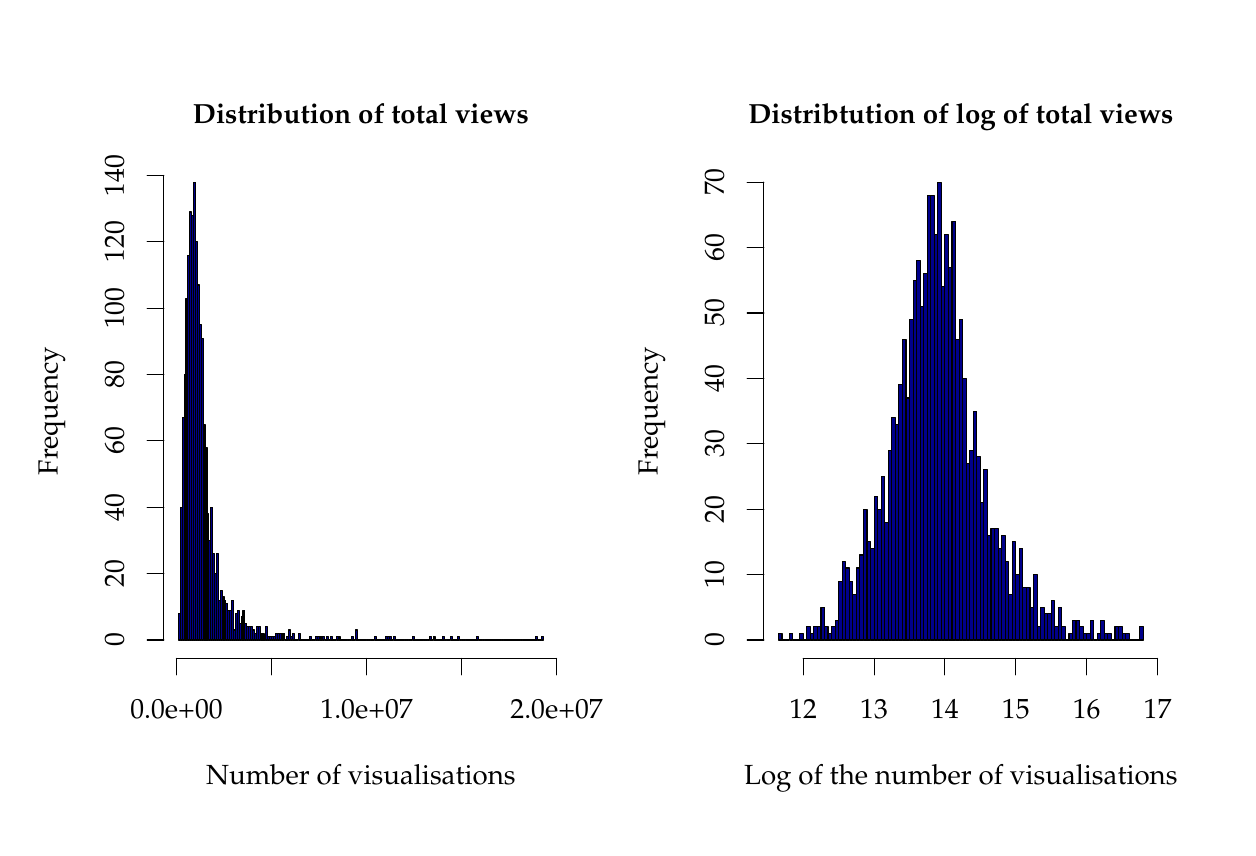
\begin{tikzpicture}[x=1pt,y=1pt]
\definecolor{fillColor}{RGB}{255,255,255}
\path[use as bounding box,fill=fillColor,fill opacity=0.00] (0,0) rectangle (433.62,289.08);
\begin{scope}
\path[clip] (  0.00,  0.00) rectangle (216.81,289.08);
\definecolor{drawColor}{RGB}{0,0,0}

\node[text=drawColor,anchor=base,inner sep=0pt, outer sep=0pt, scale=  1.00] at (120.41, 15.60) {Number of visualisations};

\node[text=drawColor,rotate= 90.00,anchor=base,inner sep=0pt, outer sep=0pt, scale=  1.00] at ( 10.80,150.54) {Frequency};
\end{scope}
\begin{scope}
\path[clip] (  0.00,  0.00) rectangle (433.62,289.08);
\definecolor{drawColor}{RGB}{0,0,0}

\path[draw=drawColor,line width= 0.4pt,line join=round,line cap=round] ( 53.79, 61.20) -- (191.14, 61.20);

\path[draw=drawColor,line width= 0.4pt,line join=round,line cap=round] ( 53.79, 61.20) -- ( 53.79, 55.20);

\path[draw=drawColor,line width= 0.4pt,line join=round,line cap=round] ( 88.13, 61.20) -- ( 88.13, 55.20);

\path[draw=drawColor,line width= 0.4pt,line join=round,line cap=round] (122.47, 61.20) -- (122.47, 55.20);

\path[draw=drawColor,line width= 0.4pt,line join=round,line cap=round] (156.80, 61.20) -- (156.80, 55.20);

\path[draw=drawColor,line width= 0.4pt,line join=round,line cap=round] (191.14, 61.20) -- (191.14, 55.20);

\node[text=drawColor,anchor=base,inner sep=0pt, outer sep=0pt, scale=  1.00] at ( 53.79, 39.60) {0.0e+00};

\node[text=drawColor,anchor=base,inner sep=0pt, outer sep=0pt, scale=  1.00] at (122.47, 39.60) {1.0e+07};

\node[text=drawColor,anchor=base,inner sep=0pt, outer sep=0pt, scale=  1.00] at (191.14, 39.60) {2.0e+07};

\path[draw=drawColor,line width= 0.4pt,line join=round,line cap=round] ( 49.20, 67.82) -- ( 49.20,235.66);

\path[draw=drawColor,line width= 0.4pt,line join=round,line cap=round] ( 49.20, 67.82) -- ( 43.20, 67.82);

\path[draw=drawColor,line width= 0.4pt,line join=round,line cap=round] ( 49.20, 91.80) -- ( 43.20, 91.80);

\path[draw=drawColor,line width= 0.4pt,line join=round,line cap=round] ( 49.20,115.77) -- ( 43.20,115.77);

\path[draw=drawColor,line width= 0.4pt,line join=round,line cap=round] ( 49.20,139.75) -- ( 43.20,139.75);

\path[draw=drawColor,line width= 0.4pt,line join=round,line cap=round] ( 49.20,163.73) -- ( 43.20,163.73);

\path[draw=drawColor,line width= 0.4pt,line join=round,line cap=round] ( 49.20,187.71) -- ( 43.20,187.71);

\path[draw=drawColor,line width= 0.4pt,line join=round,line cap=round] ( 49.20,211.68) -- ( 43.20,211.68);

\path[draw=drawColor,line width= 0.4pt,line join=round,line cap=round] ( 49.20,235.66) -- ( 43.20,235.66);

\node[text=drawColor,rotate= 90.00,anchor=base,inner sep=0pt, outer sep=0pt, scale=  1.00] at ( 34.80, 67.82) {0};

\node[text=drawColor,rotate= 90.00,anchor=base,inner sep=0pt, outer sep=0pt, scale=  1.00] at ( 34.80, 91.80) {20};

\node[text=drawColor,rotate= 90.00,anchor=base,inner sep=0pt, outer sep=0pt, scale=  1.00] at ( 34.80,115.77) {40};

\node[text=drawColor,rotate= 90.00,anchor=base,inner sep=0pt, outer sep=0pt, scale=  1.00] at ( 34.80,139.75) {60};

\node[text=drawColor,rotate= 90.00,anchor=base,inner sep=0pt, outer sep=0pt, scale=  1.00] at ( 34.80,163.73) {80};

\node[text=drawColor,rotate= 90.00,anchor=base,inner sep=0pt, outer sep=0pt, scale=  1.00] at ( 34.80,187.71) {100};

\node[text=drawColor,rotate= 90.00,anchor=base,inner sep=0pt, outer sep=0pt, scale=  1.00] at ( 34.80,211.68) {120};

\node[text=drawColor,rotate= 90.00,anchor=base,inner sep=0pt, outer sep=0pt, scale=  1.00] at ( 34.80,235.66) {140};
\end{scope}
\begin{scope}
\path[clip] ( 49.20, 61.20) rectangle (191.61,239.88);
\definecolor{drawColor}{RGB}{0,0,0}
\definecolor{fillColor}{RGB}{0,0,139}

\path[draw=drawColor,line width= 0.4pt,line join=round,line cap=round,fill=fillColor] ( 54.47, 67.82) rectangle ( 55.16, 77.41);

\path[draw=drawColor,line width= 0.4pt,line join=round,line cap=round,fill=fillColor] ( 55.16, 67.82) rectangle ( 55.85,115.77);

\path[draw=drawColor,line width= 0.4pt,line join=round,line cap=round,fill=fillColor] ( 55.85, 67.82) rectangle ( 56.53,148.14);

\path[draw=drawColor,line width= 0.4pt,line join=round,line cap=round,fill=fillColor] ( 56.53, 67.82) rectangle ( 57.22,163.73);

\path[draw=drawColor,line width= 0.4pt,line join=round,line cap=round,fill=fillColor] ( 57.22, 67.82) rectangle ( 57.91,191.30);

\path[draw=drawColor,line width= 0.4pt,line join=round,line cap=round,fill=fillColor] ( 57.91, 67.82) rectangle ( 58.60,206.89);

\path[draw=drawColor,line width= 0.4pt,line join=round,line cap=round,fill=fillColor] ( 58.60, 67.82) rectangle ( 59.28,222.47);

\path[draw=drawColor,line width= 0.4pt,line join=round,line cap=round,fill=fillColor] ( 59.28, 67.82) rectangle ( 59.97,221.27);

\path[draw=drawColor,line width= 0.4pt,line join=round,line cap=round,fill=fillColor] ( 59.97, 67.82) rectangle ( 60.66,233.26);

\path[draw=drawColor,line width= 0.4pt,line join=round,line cap=round,fill=fillColor] ( 60.66, 67.82) rectangle ( 61.34,211.68);

\path[draw=drawColor,line width= 0.4pt,line join=round,line cap=round,fill=fillColor] ( 61.34, 67.82) rectangle ( 62.03,196.10);

\path[draw=drawColor,line width= 0.4pt,line join=round,line cap=round,fill=fillColor] ( 62.03, 67.82) rectangle ( 62.72,181.71);

\path[draw=drawColor,line width= 0.4pt,line join=round,line cap=round,fill=fillColor] ( 62.72, 67.82) rectangle ( 63.40,176.92);

\path[draw=drawColor,line width= 0.4pt,line join=round,line cap=round,fill=fillColor] ( 63.40, 67.82) rectangle ( 64.09,145.74);

\path[draw=drawColor,line width= 0.4pt,line join=round,line cap=round,fill=fillColor] ( 64.09, 67.82) rectangle ( 64.78,137.35);

\path[draw=drawColor,line width= 0.4pt,line join=round,line cap=round,fill=fillColor] ( 64.78, 67.82) rectangle ( 65.46,113.37);

\path[draw=drawColor,line width= 0.4pt,line join=round,line cap=round,fill=fillColor] ( 65.46, 67.82) rectangle ( 66.15,103.78);

\path[draw=drawColor,line width= 0.4pt,line join=round,line cap=round,fill=fillColor] ( 66.15, 67.82) rectangle ( 66.84,115.77);

\path[draw=drawColor,line width= 0.4pt,line join=round,line cap=round,fill=fillColor] ( 66.84, 67.82) rectangle ( 67.52, 98.99);

\path[draw=drawColor,line width= 0.4pt,line join=round,line cap=round,fill=fillColor] ( 67.52, 67.82) rectangle ( 68.21, 91.80);

\path[draw=drawColor,line width= 0.4pt,line join=round,line cap=round,fill=fillColor] ( 68.21, 67.82) rectangle ( 68.90, 98.99);

\path[draw=drawColor,line width= 0.4pt,line join=round,line cap=round,fill=fillColor] ( 68.90, 67.82) rectangle ( 69.58, 82.20);

\path[draw=drawColor,line width= 0.4pt,line join=round,line cap=round,fill=fillColor] ( 69.58, 67.82) rectangle ( 70.27, 85.80);

\path[draw=drawColor,line width= 0.4pt,line join=round,line cap=round,fill=fillColor] ( 70.27, 67.82) rectangle ( 70.96, 83.40);

\path[draw=drawColor,line width= 0.4pt,line join=round,line cap=round,fill=fillColor] ( 70.96, 67.82) rectangle ( 71.64, 82.20);

\path[draw=drawColor,line width= 0.4pt,line join=round,line cap=round,fill=fillColor] ( 71.64, 67.82) rectangle ( 72.33, 81.01);

\path[draw=drawColor,line width= 0.4pt,line join=round,line cap=round,fill=fillColor] ( 72.33, 67.82) rectangle ( 73.02, 78.61);

\path[draw=drawColor,line width= 0.4pt,line join=round,line cap=round,fill=fillColor] ( 73.02, 67.82) rectangle ( 73.70, 78.61);

\path[draw=drawColor,line width= 0.4pt,line join=round,line cap=round,fill=fillColor] ( 73.70, 67.82) rectangle ( 74.39, 82.20);

\path[draw=drawColor,line width= 0.4pt,line join=round,line cap=round,fill=fillColor] ( 74.39, 67.82) rectangle ( 75.08, 71.41);

\path[draw=drawColor,line width= 0.4pt,line join=round,line cap=round,fill=fillColor] ( 75.08, 67.82) rectangle ( 75.76, 77.41);

\path[draw=drawColor,line width= 0.4pt,line join=round,line cap=round,fill=fillColor] ( 75.76, 67.82) rectangle ( 76.45, 78.61);

\path[draw=drawColor,line width= 0.4pt,line join=round,line cap=round,fill=fillColor] ( 76.45, 67.82) rectangle ( 77.14, 73.81);

\path[draw=drawColor,line width= 0.4pt,line join=round,line cap=round,fill=fillColor] ( 77.14, 67.82) rectangle ( 77.82, 76.21);

\path[draw=drawColor,line width= 0.4pt,line join=round,line cap=round,fill=fillColor] ( 77.82, 67.82) rectangle ( 78.51, 78.61);

\path[draw=drawColor,line width= 0.4pt,line join=round,line cap=round,fill=fillColor] ( 78.51, 67.82) rectangle ( 79.20, 73.81);

\path[draw=drawColor,line width= 0.4pt,line join=round,line cap=round,fill=fillColor] ( 79.20, 67.82) rectangle ( 79.89, 72.61);

\path[draw=drawColor,line width= 0.4pt,line join=round,line cap=round,fill=fillColor] ( 79.89, 67.82) rectangle ( 80.57, 72.61);

\path[draw=drawColor,line width= 0.4pt,line join=round,line cap=round,fill=fillColor] ( 80.57, 67.82) rectangle ( 81.26, 72.61);

\path[draw=drawColor,line width= 0.4pt,line join=round,line cap=round,fill=fillColor] ( 81.26, 67.82) rectangle ( 81.95, 71.41);

\path[draw=drawColor,line width= 0.4pt,line join=round,line cap=round,fill=fillColor] ( 81.95, 67.82) rectangle ( 82.63, 70.22);

\path[draw=drawColor,line width= 0.4pt,line join=round,line cap=round,fill=fillColor] ( 82.63, 67.82) rectangle ( 83.32, 72.61);

\path[draw=drawColor,line width= 0.4pt,line join=round,line cap=round,fill=fillColor] ( 83.32, 67.82) rectangle ( 84.01, 72.61);

\path[draw=drawColor,line width= 0.4pt,line join=round,line cap=round,fill=fillColor] ( 84.01, 67.82) rectangle ( 84.69, 70.22);

\path[draw=drawColor,line width= 0.4pt,line join=round,line cap=round,fill=fillColor] ( 84.69, 67.82) rectangle ( 85.38, 70.22);

\path[draw=drawColor,line width= 0.4pt,line join=round,line cap=round,fill=fillColor] ( 85.38, 67.82) rectangle ( 86.07, 69.02);

\path[draw=drawColor,line width= 0.4pt,line join=round,line cap=round,fill=fillColor] ( 86.07, 67.82) rectangle ( 86.75, 72.61);

\path[draw=drawColor,line width= 0.4pt,line join=round,line cap=round,fill=fillColor] ( 86.75, 67.82) rectangle ( 87.44, 69.02);

\path[draw=drawColor,line width= 0.4pt,line join=round,line cap=round,fill=fillColor] ( 87.44, 67.82) rectangle ( 88.13, 69.02);

\path[draw=drawColor,line width= 0.4pt,line join=round,line cap=round,fill=fillColor] ( 88.13, 67.82) rectangle ( 88.81, 69.02);

\path[draw=drawColor,line width= 0.4pt,line join=round,line cap=round,fill=fillColor] ( 88.81, 67.82) rectangle ( 89.50, 69.02);

\path[draw=drawColor,line width= 0.4pt,line join=round,line cap=round,fill=fillColor] ( 89.50, 67.82) rectangle ( 90.19, 70.22);

\path[draw=drawColor,line width= 0.4pt,line join=round,line cap=round,fill=fillColor] ( 90.19, 67.82) rectangle ( 90.87, 70.22);

\path[draw=drawColor,line width= 0.4pt,line join=round,line cap=round,fill=fillColor] ( 90.87, 67.82) rectangle ( 91.56, 70.22);

\path[draw=drawColor,line width= 0.4pt,line join=round,line cap=round,fill=fillColor] ( 91.56, 67.82) rectangle ( 92.25, 70.22);

\path[draw=drawColor,line width= 0.4pt,line join=round,line cap=round,fill=fillColor] ( 92.25, 67.82) rectangle ( 92.93, 70.22);

\path[draw=drawColor,line width= 0.4pt,line join=round,line cap=round,fill=fillColor] ( 92.93, 67.82) rectangle ( 93.62, 67.82);

\path[draw=drawColor,line width= 0.4pt,line join=round,line cap=round,fill=fillColor] ( 93.62, 67.82) rectangle ( 94.31, 69.02);

\path[draw=drawColor,line width= 0.4pt,line join=round,line cap=round,fill=fillColor] ( 94.31, 67.82) rectangle ( 94.99, 71.41);

\path[draw=drawColor,line width= 0.4pt,line join=round,line cap=round,fill=fillColor] ( 94.99, 67.82) rectangle ( 95.68, 69.02);

\path[draw=drawColor,line width= 0.4pt,line join=round,line cap=round,fill=fillColor] ( 95.68, 67.82) rectangle ( 96.37, 70.22);

\path[draw=drawColor,line width= 0.4pt,line join=round,line cap=round,fill=fillColor] ( 96.37, 67.82) rectangle ( 97.05, 67.82);

\path[draw=drawColor,line width= 0.4pt,line join=round,line cap=round,fill=fillColor] ( 97.05, 67.82) rectangle ( 97.74, 67.82);

\path[draw=drawColor,line width= 0.4pt,line join=round,line cap=round,fill=fillColor] ( 97.74, 67.82) rectangle ( 98.43, 70.22);

\path[draw=drawColor,line width= 0.4pt,line join=round,line cap=round,fill=fillColor] ( 98.43, 67.82) rectangle ( 99.11, 67.82);

\path[draw=drawColor,line width= 0.4pt,line join=round,line cap=round,fill=fillColor] ( 99.11, 67.82) rectangle ( 99.80, 67.82);

\path[draw=drawColor,line width= 0.4pt,line join=round,line cap=round,fill=fillColor] ( 99.80, 67.82) rectangle (100.49, 67.82);

\path[draw=drawColor,line width= 0.4pt,line join=round,line cap=round,fill=fillColor] (100.49, 67.82) rectangle (101.18, 67.82);

\path[draw=drawColor,line width= 0.4pt,line join=round,line cap=round,fill=fillColor] (101.18, 67.82) rectangle (101.86, 67.82);

\path[draw=drawColor,line width= 0.4pt,line join=round,line cap=round,fill=fillColor] (101.86, 67.82) rectangle (102.55, 69.02);

\path[draw=drawColor,line width= 0.4pt,line join=round,line cap=round,fill=fillColor] (102.55, 67.82) rectangle (103.24, 67.82);

\path[draw=drawColor,line width= 0.4pt,line join=round,line cap=round,fill=fillColor] (103.24, 67.82) rectangle (103.92, 67.82);

\path[draw=drawColor,line width= 0.4pt,line join=round,line cap=round,fill=fillColor] (103.92, 67.82) rectangle (104.61, 69.02);

\path[draw=drawColor,line width= 0.4pt,line join=round,line cap=round,fill=fillColor] (104.61, 67.82) rectangle (105.30, 69.02);

\path[draw=drawColor,line width= 0.4pt,line join=round,line cap=round,fill=fillColor] (105.30, 67.82) rectangle (105.98, 69.02);

\path[draw=drawColor,line width= 0.4pt,line join=round,line cap=round,fill=fillColor] (105.98, 67.82) rectangle (106.67, 69.02);

\path[draw=drawColor,line width= 0.4pt,line join=round,line cap=round,fill=fillColor] (106.67, 67.82) rectangle (107.36, 69.02);

\path[draw=drawColor,line width= 0.4pt,line join=round,line cap=round,fill=fillColor] (107.36, 67.82) rectangle (108.04, 67.82);

\path[draw=drawColor,line width= 0.4pt,line join=round,line cap=round,fill=fillColor] (108.04, 67.82) rectangle (108.73, 69.02);

\path[draw=drawColor,line width= 0.4pt,line join=round,line cap=round,fill=fillColor] (108.73, 67.82) rectangle (109.42, 67.82);

\path[draw=drawColor,line width= 0.4pt,line join=round,line cap=round,fill=fillColor] (109.42, 67.82) rectangle (110.10, 69.02);

\path[draw=drawColor,line width= 0.4pt,line join=round,line cap=round,fill=fillColor] (110.10, 67.82) rectangle (110.79, 67.82);

\path[draw=drawColor,line width= 0.4pt,line join=round,line cap=round,fill=fillColor] (110.79, 67.82) rectangle (111.48, 67.82);

\path[draw=drawColor,line width= 0.4pt,line join=round,line cap=round,fill=fillColor] (111.48, 67.82) rectangle (112.16, 69.02);

\path[draw=drawColor,line width= 0.4pt,line join=round,line cap=round,fill=fillColor] (112.16, 67.82) rectangle (112.85, 69.02);

\path[draw=drawColor,line width= 0.4pt,line join=round,line cap=round,fill=fillColor] (112.85, 67.82) rectangle (113.54, 67.82);

\path[draw=drawColor,line width= 0.4pt,line join=round,line cap=round,fill=fillColor] (113.54, 67.82) rectangle (114.22, 67.82);

\path[draw=drawColor,line width= 0.4pt,line join=round,line cap=round,fill=fillColor] (114.22, 67.82) rectangle (114.91, 67.82);

\path[draw=drawColor,line width= 0.4pt,line join=round,line cap=round,fill=fillColor] (114.91, 67.82) rectangle (115.60, 67.82);

\path[draw=drawColor,line width= 0.4pt,line join=round,line cap=round,fill=fillColor] (115.60, 67.82) rectangle (116.28, 67.82);

\path[draw=drawColor,line width= 0.4pt,line join=round,line cap=round,fill=fillColor] (116.28, 67.82) rectangle (116.97, 67.82);

\path[draw=drawColor,line width= 0.4pt,line join=round,line cap=round,fill=fillColor] (116.97, 67.82) rectangle (117.66, 69.02);

\path[draw=drawColor,line width= 0.4pt,line join=round,line cap=round,fill=fillColor] (117.66, 67.82) rectangle (118.34, 67.82);

\path[draw=drawColor,line width= 0.4pt,line join=round,line cap=round,fill=fillColor] (118.34, 67.82) rectangle (119.03, 71.41);

\path[draw=drawColor,line width= 0.4pt,line join=round,line cap=round,fill=fillColor] (119.03, 67.82) rectangle (119.72, 67.82);

\path[draw=drawColor,line width= 0.4pt,line join=round,line cap=round,fill=fillColor] (119.72, 67.82) rectangle (120.41, 67.82);

\path[draw=drawColor,line width= 0.4pt,line join=round,line cap=round,fill=fillColor] (120.41, 67.82) rectangle (121.09, 67.82);

\path[draw=drawColor,line width= 0.4pt,line join=round,line cap=round,fill=fillColor] (121.09, 67.82) rectangle (121.78, 67.82);

\path[draw=drawColor,line width= 0.4pt,line join=round,line cap=round,fill=fillColor] (121.78, 67.82) rectangle (122.47, 67.82);

\path[draw=drawColor,line width= 0.4pt,line join=round,line cap=round,fill=fillColor] (122.47, 67.82) rectangle (123.15, 67.82);

\path[draw=drawColor,line width= 0.4pt,line join=round,line cap=round,fill=fillColor] (123.15, 67.82) rectangle (123.84, 67.82);

\path[draw=drawColor,line width= 0.4pt,line join=round,line cap=round,fill=fillColor] (123.84, 67.82) rectangle (124.53, 67.82);

\path[draw=drawColor,line width= 0.4pt,line join=round,line cap=round,fill=fillColor] (124.53, 67.82) rectangle (125.21, 67.82);

\path[draw=drawColor,line width= 0.4pt,line join=round,line cap=round,fill=fillColor] (125.21, 67.82) rectangle (125.90, 69.02);

\path[draw=drawColor,line width= 0.4pt,line join=round,line cap=round,fill=fillColor] (125.90, 67.82) rectangle (126.59, 67.82);

\path[draw=drawColor,line width= 0.4pt,line join=round,line cap=round,fill=fillColor] (126.59, 67.82) rectangle (127.27, 67.82);

\path[draw=drawColor,line width= 0.4pt,line join=round,line cap=round,fill=fillColor] (127.27, 67.82) rectangle (127.96, 67.82);

\path[draw=drawColor,line width= 0.4pt,line join=round,line cap=round,fill=fillColor] (127.96, 67.82) rectangle (128.65, 67.82);

\path[draw=drawColor,line width= 0.4pt,line join=round,line cap=round,fill=fillColor] (128.65, 67.82) rectangle (129.33, 67.82);

\path[draw=drawColor,line width= 0.4pt,line join=round,line cap=round,fill=fillColor] (129.33, 67.82) rectangle (130.02, 69.02);

\path[draw=drawColor,line width= 0.4pt,line join=round,line cap=round,fill=fillColor] (130.02, 67.82) rectangle (130.71, 69.02);

\path[draw=drawColor,line width= 0.4pt,line join=round,line cap=round,fill=fillColor] (130.71, 67.82) rectangle (131.39, 69.02);

\path[draw=drawColor,line width= 0.4pt,line join=round,line cap=round,fill=fillColor] (131.39, 67.82) rectangle (132.08, 67.82);

\path[draw=drawColor,line width= 0.4pt,line join=round,line cap=round,fill=fillColor] (132.08, 67.82) rectangle (132.77, 69.02);

\path[draw=drawColor,line width= 0.4pt,line join=round,line cap=round,fill=fillColor] (132.77, 67.82) rectangle (133.45, 67.82);

\path[draw=drawColor,line width= 0.4pt,line join=round,line cap=round,fill=fillColor] (133.45, 67.82) rectangle (134.14, 67.82);

\path[draw=drawColor,line width= 0.4pt,line join=round,line cap=round,fill=fillColor] (134.14, 67.82) rectangle (134.83, 67.82);

\path[draw=drawColor,line width= 0.4pt,line join=round,line cap=round,fill=fillColor] (134.83, 67.82) rectangle (135.51, 67.82);

\path[draw=drawColor,line width= 0.4pt,line join=round,line cap=round,fill=fillColor] (135.51, 67.82) rectangle (136.20, 67.82);

\path[draw=drawColor,line width= 0.4pt,line join=round,line cap=round,fill=fillColor] (136.20, 67.82) rectangle (136.89, 67.82);

\path[draw=drawColor,line width= 0.4pt,line join=round,line cap=round,fill=fillColor] (136.89, 67.82) rectangle (137.57, 67.82);

\path[draw=drawColor,line width= 0.4pt,line join=round,line cap=round,fill=fillColor] (137.57, 67.82) rectangle (138.26, 67.82);

\path[draw=drawColor,line width= 0.4pt,line join=round,line cap=round,fill=fillColor] (138.26, 67.82) rectangle (138.95, 67.82);

\path[draw=drawColor,line width= 0.4pt,line join=round,line cap=round,fill=fillColor] (138.95, 67.82) rectangle (139.63, 69.02);

\path[draw=drawColor,line width= 0.4pt,line join=round,line cap=round,fill=fillColor] (139.63, 67.82) rectangle (140.32, 67.82);

\path[draw=drawColor,line width= 0.4pt,line join=round,line cap=round,fill=fillColor] (140.32, 67.82) rectangle (141.01, 67.82);

\path[draw=drawColor,line width= 0.4pt,line join=round,line cap=round,fill=fillColor] (141.01, 67.82) rectangle (141.70, 67.82);

\path[draw=drawColor,line width= 0.4pt,line join=round,line cap=round,fill=fillColor] (141.70, 67.82) rectangle (142.38, 67.82);

\path[draw=drawColor,line width= 0.4pt,line join=round,line cap=round,fill=fillColor] (142.38, 67.82) rectangle (143.07, 67.82);

\path[draw=drawColor,line width= 0.4pt,line join=round,line cap=round,fill=fillColor] (143.07, 67.82) rectangle (143.76, 67.82);

\path[draw=drawColor,line width= 0.4pt,line join=round,line cap=round,fill=fillColor] (143.76, 67.82) rectangle (144.44, 67.82);

\path[draw=drawColor,line width= 0.4pt,line join=round,line cap=round,fill=fillColor] (144.44, 67.82) rectangle (145.13, 67.82);

\path[draw=drawColor,line width= 0.4pt,line join=round,line cap=round,fill=fillColor] (145.13, 67.82) rectangle (145.82, 69.02);

\path[draw=drawColor,line width= 0.4pt,line join=round,line cap=round,fill=fillColor] (145.82, 67.82) rectangle (146.50, 67.82);

\path[draw=drawColor,line width= 0.4pt,line join=round,line cap=round,fill=fillColor] (146.50, 67.82) rectangle (147.19, 69.02);

\path[draw=drawColor,line width= 0.4pt,line join=round,line cap=round,fill=fillColor] (147.19, 67.82) rectangle (147.88, 67.82);

\path[draw=drawColor,line width= 0.4pt,line join=round,line cap=round,fill=fillColor] (147.88, 67.82) rectangle (148.56, 67.82);

\path[draw=drawColor,line width= 0.4pt,line join=round,line cap=round,fill=fillColor] (148.56, 67.82) rectangle (149.25, 67.82);

\path[draw=drawColor,line width= 0.4pt,line join=round,line cap=round,fill=fillColor] (149.25, 67.82) rectangle (149.94, 67.82);

\path[draw=drawColor,line width= 0.4pt,line join=round,line cap=round,fill=fillColor] (149.94, 67.82) rectangle (150.62, 69.02);

\path[draw=drawColor,line width= 0.4pt,line join=round,line cap=round,fill=fillColor] (150.62, 67.82) rectangle (151.31, 67.82);

\path[draw=drawColor,line width= 0.4pt,line join=round,line cap=round,fill=fillColor] (151.31, 67.82) rectangle (152.00, 67.82);

\path[draw=drawColor,line width= 0.4pt,line join=round,line cap=round,fill=fillColor] (152.00, 67.82) rectangle (152.68, 67.82);

\path[draw=drawColor,line width= 0.4pt,line join=round,line cap=round,fill=fillColor] (152.68, 67.82) rectangle (153.37, 69.02);

\path[draw=drawColor,line width= 0.4pt,line join=round,line cap=round,fill=fillColor] (153.37, 67.82) rectangle (154.06, 67.82);

\path[draw=drawColor,line width= 0.4pt,line join=round,line cap=round,fill=fillColor] (154.06, 67.82) rectangle (154.74, 67.82);

\path[draw=drawColor,line width= 0.4pt,line join=round,line cap=round,fill=fillColor] (154.74, 67.82) rectangle (155.43, 67.82);

\path[draw=drawColor,line width= 0.4pt,line join=round,line cap=round,fill=fillColor] (155.43, 67.82) rectangle (156.12, 69.02);

\path[draw=drawColor,line width= 0.4pt,line join=round,line cap=round,fill=fillColor] (156.12, 67.82) rectangle (156.80, 67.82);

\path[draw=drawColor,line width= 0.4pt,line join=round,line cap=round,fill=fillColor] (156.80, 67.82) rectangle (157.49, 67.82);

\path[draw=drawColor,line width= 0.4pt,line join=round,line cap=round,fill=fillColor] (157.49, 67.82) rectangle (158.18, 67.82);

\path[draw=drawColor,line width= 0.4pt,line join=round,line cap=round,fill=fillColor] (158.18, 67.82) rectangle (158.86, 67.82);

\path[draw=drawColor,line width= 0.4pt,line join=round,line cap=round,fill=fillColor] (158.86, 67.82) rectangle (159.55, 67.82);

\path[draw=drawColor,line width= 0.4pt,line join=round,line cap=round,fill=fillColor] (159.55, 67.82) rectangle (160.24, 67.82);

\path[draw=drawColor,line width= 0.4pt,line join=round,line cap=round,fill=fillColor] (160.24, 67.82) rectangle (160.92, 67.82);

\path[draw=drawColor,line width= 0.4pt,line join=round,line cap=round,fill=fillColor] (160.92, 67.82) rectangle (161.61, 67.82);

\path[draw=drawColor,line width= 0.4pt,line join=round,line cap=round,fill=fillColor] (161.61, 67.82) rectangle (162.30, 67.82);

\path[draw=drawColor,line width= 0.4pt,line join=round,line cap=round,fill=fillColor] (162.30, 67.82) rectangle (162.99, 69.02);

\path[draw=drawColor,line width= 0.4pt,line join=round,line cap=round,fill=fillColor] (162.99, 67.82) rectangle (163.67, 67.82);

\path[draw=drawColor,line width= 0.4pt,line join=round,line cap=round,fill=fillColor] (163.67, 67.82) rectangle (164.36, 67.82);

\path[draw=drawColor,line width= 0.4pt,line join=round,line cap=round,fill=fillColor] (164.36, 67.82) rectangle (165.05, 67.82);

\path[draw=drawColor,line width= 0.4pt,line join=round,line cap=round,fill=fillColor] (165.05, 67.82) rectangle (165.73, 67.82);

\path[draw=drawColor,line width= 0.4pt,line join=round,line cap=round,fill=fillColor] (165.73, 67.82) rectangle (166.42, 67.82);

\path[draw=drawColor,line width= 0.4pt,line join=round,line cap=round,fill=fillColor] (166.42, 67.82) rectangle (167.11, 67.82);

\path[draw=drawColor,line width= 0.4pt,line join=round,line cap=round,fill=fillColor] (167.11, 67.82) rectangle (167.79, 67.82);

\path[draw=drawColor,line width= 0.4pt,line join=round,line cap=round,fill=fillColor] (167.79, 67.82) rectangle (168.48, 67.82);

\path[draw=drawColor,line width= 0.4pt,line join=round,line cap=round,fill=fillColor] (168.48, 67.82) rectangle (169.17, 67.82);

\path[draw=drawColor,line width= 0.4pt,line join=round,line cap=round,fill=fillColor] (169.17, 67.82) rectangle (169.85, 67.82);

\path[draw=drawColor,line width= 0.4pt,line join=round,line cap=round,fill=fillColor] (169.85, 67.82) rectangle (170.54, 67.82);

\path[draw=drawColor,line width= 0.4pt,line join=round,line cap=round,fill=fillColor] (170.54, 67.82) rectangle (171.23, 67.82);

\path[draw=drawColor,line width= 0.4pt,line join=round,line cap=round,fill=fillColor] (171.23, 67.82) rectangle (171.91, 67.82);

\path[draw=drawColor,line width= 0.4pt,line join=round,line cap=round,fill=fillColor] (171.91, 67.82) rectangle (172.60, 67.82);

\path[draw=drawColor,line width= 0.4pt,line join=round,line cap=round,fill=fillColor] (172.60, 67.82) rectangle (173.29, 67.82);

\path[draw=drawColor,line width= 0.4pt,line join=round,line cap=round,fill=fillColor] (173.29, 67.82) rectangle (173.97, 67.82);

\path[draw=drawColor,line width= 0.4pt,line join=round,line cap=round,fill=fillColor] (173.97, 67.82) rectangle (174.66, 67.82);

\path[draw=drawColor,line width= 0.4pt,line join=round,line cap=round,fill=fillColor] (174.66, 67.82) rectangle (175.35, 67.82);

\path[draw=drawColor,line width= 0.4pt,line join=round,line cap=round,fill=fillColor] (175.35, 67.82) rectangle (176.03, 67.82);

\path[draw=drawColor,line width= 0.4pt,line join=round,line cap=round,fill=fillColor] (176.03, 67.82) rectangle (176.72, 67.82);

\path[draw=drawColor,line width= 0.4pt,line join=round,line cap=round,fill=fillColor] (176.72, 67.82) rectangle (177.41, 67.82);

\path[draw=drawColor,line width= 0.4pt,line join=round,line cap=round,fill=fillColor] (177.41, 67.82) rectangle (178.09, 67.82);

\path[draw=drawColor,line width= 0.4pt,line join=round,line cap=round,fill=fillColor] (178.09, 67.82) rectangle (178.78, 67.82);

\path[draw=drawColor,line width= 0.4pt,line join=round,line cap=round,fill=fillColor] (178.78, 67.82) rectangle (179.47, 67.82);

\path[draw=drawColor,line width= 0.4pt,line join=round,line cap=round,fill=fillColor] (179.47, 67.82) rectangle (180.15, 67.82);

\path[draw=drawColor,line width= 0.4pt,line join=round,line cap=round,fill=fillColor] (180.15, 67.82) rectangle (180.84, 67.82);

\path[draw=drawColor,line width= 0.4pt,line join=round,line cap=round,fill=fillColor] (180.84, 67.82) rectangle (181.53, 67.82);

\path[draw=drawColor,line width= 0.4pt,line join=round,line cap=round,fill=fillColor] (181.53, 67.82) rectangle (182.21, 67.82);

\path[draw=drawColor,line width= 0.4pt,line join=round,line cap=round,fill=fillColor] (182.21, 67.82) rectangle (182.90, 67.82);

\path[draw=drawColor,line width= 0.4pt,line join=round,line cap=round,fill=fillColor] (182.90, 67.82) rectangle (183.59, 67.82);

\path[draw=drawColor,line width= 0.4pt,line join=round,line cap=round,fill=fillColor] (183.59, 67.82) rectangle (184.28, 69.02);

\path[draw=drawColor,line width= 0.4pt,line join=round,line cap=round,fill=fillColor] (184.28, 67.82) rectangle (184.96, 67.82);

\path[draw=drawColor,line width= 0.4pt,line join=round,line cap=round,fill=fillColor] (184.96, 67.82) rectangle (185.65, 67.82);

\path[draw=drawColor,line width= 0.4pt,line join=round,line cap=round,fill=fillColor] (185.65, 67.82) rectangle (186.34, 69.02);
\end{scope}
\begin{scope}
\path[clip] (  0.00,  0.00) rectangle (433.62,289.08);
\definecolor{drawColor}{RGB}{0,0,0}

\node[text=drawColor,anchor=base,inner sep=0pt, outer sep=0pt, scale=  1.00] at (120.41,254.28) {\textbf{Distribution of total views}};
\end{scope}
\begin{scope}
\path[clip] (216.81,  0.00) rectangle (433.62,289.08);
\definecolor{drawColor}{RGB}{0,0,0}

\node[text=drawColor,anchor=base,inner sep=0pt, outer sep=0pt, scale=  1.00] at (337.21, 15.60) {Log of the number of visualisations};

\node[text=drawColor,rotate= 90.00,anchor=base,inner sep=0pt, outer sep=0pt, scale=  1.00] at (227.61,150.54) {Frequency};
\end{scope}
\begin{scope}
\path[clip] (  0.00,  0.00) rectangle (433.62,289.08);
\definecolor{drawColor}{RGB}{0,0,0}

\path[draw=drawColor,line width= 0.4pt,line join=round,line cap=round] (280.25, 61.20) -- (408.27, 61.20);

\path[draw=drawColor,line width= 0.4pt,line join=round,line cap=round] (280.25, 61.20) -- (280.25, 55.20);

\path[draw=drawColor,line width= 0.4pt,line join=round,line cap=round] (305.85, 61.20) -- (305.85, 55.20);

\path[draw=drawColor,line width= 0.4pt,line join=round,line cap=round] (331.45, 61.20) -- (331.45, 55.20);

\path[draw=drawColor,line width= 0.4pt,line join=round,line cap=round] (357.06, 61.20) -- (357.06, 55.20);

\path[draw=drawColor,line width= 0.4pt,line join=round,line cap=round] (382.66, 61.20) -- (382.66, 55.20);

\path[draw=drawColor,line width= 0.4pt,line join=round,line cap=round] (408.27, 61.20) -- (408.27, 55.20);

\node[text=drawColor,anchor=base,inner sep=0pt, outer sep=0pt, scale=  1.00] at (280.25, 39.60) {12};

\node[text=drawColor,anchor=base,inner sep=0pt, outer sep=0pt, scale=  1.00] at (305.85, 39.60) {13};

\node[text=drawColor,anchor=base,inner sep=0pt, outer sep=0pt, scale=  1.00] at (331.45, 39.60) {14};

\node[text=drawColor,anchor=base,inner sep=0pt, outer sep=0pt, scale=  1.00] at (357.06, 39.60) {15};

\node[text=drawColor,anchor=base,inner sep=0pt, outer sep=0pt, scale=  1.00] at (382.66, 39.60) {16};

\node[text=drawColor,anchor=base,inner sep=0pt, outer sep=0pt, scale=  1.00] at (408.27, 39.60) {17};

\path[draw=drawColor,line width= 0.4pt,line join=round,line cap=round] (266.01, 67.82) -- (266.01,233.26);

\path[draw=drawColor,line width= 0.4pt,line join=round,line cap=round] (266.01, 67.82) -- (260.01, 67.82);

\path[draw=drawColor,line width= 0.4pt,line join=round,line cap=round] (266.01, 91.45) -- (260.01, 91.45);

\path[draw=drawColor,line width= 0.4pt,line join=round,line cap=round] (266.01,115.09) -- (260.01,115.09);

\path[draw=drawColor,line width= 0.4pt,line join=round,line cap=round] (266.01,138.72) -- (260.01,138.72);

\path[draw=drawColor,line width= 0.4pt,line join=round,line cap=round] (266.01,162.36) -- (260.01,162.36);

\path[draw=drawColor,line width= 0.4pt,line join=round,line cap=round] (266.01,185.99) -- (260.01,185.99);

\path[draw=drawColor,line width= 0.4pt,line join=round,line cap=round] (266.01,209.63) -- (260.01,209.63);

\path[draw=drawColor,line width= 0.4pt,line join=round,line cap=round] (266.01,233.26) -- (260.01,233.26);

\node[text=drawColor,rotate= 90.00,anchor=base,inner sep=0pt, outer sep=0pt, scale=  1.00] at (251.61, 67.82) {0};

\node[text=drawColor,rotate= 90.00,anchor=base,inner sep=0pt, outer sep=0pt, scale=  1.00] at (251.61, 91.45) {10};

\node[text=drawColor,rotate= 90.00,anchor=base,inner sep=0pt, outer sep=0pt, scale=  1.00] at (251.61,115.09) {20};

\node[text=drawColor,rotate= 90.00,anchor=base,inner sep=0pt, outer sep=0pt, scale=  1.00] at (251.61,138.72) {30};

\node[text=drawColor,rotate= 90.00,anchor=base,inner sep=0pt, outer sep=0pt, scale=  1.00] at (251.61,162.36) {40};

\node[text=drawColor,rotate= 90.00,anchor=base,inner sep=0pt, outer sep=0pt, scale=  1.00] at (251.61,185.99) {50};

\node[text=drawColor,rotate= 90.00,anchor=base,inner sep=0pt, outer sep=0pt, scale=  1.00] at (251.61,209.63) {60};

\node[text=drawColor,rotate= 90.00,anchor=base,inner sep=0pt, outer sep=0pt, scale=  1.00] at (251.61,233.26) {70};
\end{scope}
\begin{scope}
\path[clip] (266.01, 61.20) rectangle (408.42,239.88);
\definecolor{drawColor}{RGB}{0,0,0}
\definecolor{fillColor}{RGB}{0,0,139}

\path[draw=drawColor,line width= 0.4pt,line join=round,line cap=round,fill=fillColor] (271.28, 67.82) rectangle (272.56, 70.18);

\path[draw=drawColor,line width= 0.4pt,line join=round,line cap=round,fill=fillColor] (272.56, 67.82) rectangle (273.84, 67.82);

\path[draw=drawColor,line width= 0.4pt,line join=round,line cap=round,fill=fillColor] (273.84, 67.82) rectangle (275.13, 67.82);

\path[draw=drawColor,line width= 0.4pt,line join=round,line cap=round,fill=fillColor] (275.13, 67.82) rectangle (276.41, 70.18);

\path[draw=drawColor,line width= 0.4pt,line join=round,line cap=round,fill=fillColor] (276.41, 67.82) rectangle (277.69, 67.82);

\path[draw=drawColor,line width= 0.4pt,line join=round,line cap=round,fill=fillColor] (277.69, 67.82) rectangle (278.97, 67.82);

\path[draw=drawColor,line width= 0.4pt,line join=round,line cap=round,fill=fillColor] (278.97, 67.82) rectangle (280.25, 70.18);

\path[draw=drawColor,line width= 0.4pt,line join=round,line cap=round,fill=fillColor] (280.25, 67.82) rectangle (281.53, 67.82);

\path[draw=drawColor,line width= 0.4pt,line join=round,line cap=round,fill=fillColor] (281.53, 67.82) rectangle (282.81, 72.54);

\path[draw=drawColor,line width= 0.4pt,line join=round,line cap=round,fill=fillColor] (282.81, 67.82) rectangle (284.09, 70.18);

\path[draw=drawColor,line width= 0.4pt,line join=round,line cap=round,fill=fillColor] (284.09, 67.82) rectangle (285.37, 72.54);

\path[draw=drawColor,line width= 0.4pt,line join=round,line cap=round,fill=fillColor] (285.37, 67.82) rectangle (286.65, 72.54);

\path[draw=drawColor,line width= 0.4pt,line join=round,line cap=round,fill=fillColor] (286.65, 67.82) rectangle (287.93, 79.64);

\path[draw=drawColor,line width= 0.4pt,line join=round,line cap=round,fill=fillColor] (287.93, 67.82) rectangle (289.21, 72.54);

\path[draw=drawColor,line width= 0.4pt,line join=round,line cap=round,fill=fillColor] (289.21, 67.82) rectangle (290.49, 70.18);

\path[draw=drawColor,line width= 0.4pt,line join=round,line cap=round,fill=fillColor] (290.49, 67.82) rectangle (291.77, 72.54);

\path[draw=drawColor,line width= 0.4pt,line join=round,line cap=round,fill=fillColor] (291.77, 67.82) rectangle (293.05, 74.91);

\path[draw=drawColor,line width= 0.4pt,line join=round,line cap=round,fill=fillColor] (293.05, 67.82) rectangle (294.33, 89.09);

\path[draw=drawColor,line width= 0.4pt,line join=round,line cap=round,fill=fillColor] (294.33, 67.82) rectangle (295.61, 96.18);

\path[draw=drawColor,line width= 0.4pt,line join=round,line cap=round,fill=fillColor] (295.61, 67.82) rectangle (296.89, 93.82);

\path[draw=drawColor,line width= 0.4pt,line join=round,line cap=round,fill=fillColor] (296.89, 67.82) rectangle (298.17, 89.09);

\path[draw=drawColor,line width= 0.4pt,line join=round,line cap=round,fill=fillColor] (298.17, 67.82) rectangle (299.45, 84.36);

\path[draw=drawColor,line width= 0.4pt,line join=round,line cap=round,fill=fillColor] (299.45, 67.82) rectangle (300.73, 93.82);

\path[draw=drawColor,line width= 0.4pt,line join=round,line cap=round,fill=fillColor] (300.73, 67.82) rectangle (302.01, 98.54);

\path[draw=drawColor,line width= 0.4pt,line join=round,line cap=round,fill=fillColor] (302.01, 67.82) rectangle (303.29,115.09);

\path[draw=drawColor,line width= 0.4pt,line join=round,line cap=round,fill=fillColor] (303.29, 67.82) rectangle (304.57,103.27);

\path[draw=drawColor,line width= 0.4pt,line join=round,line cap=round,fill=fillColor] (304.57, 67.82) rectangle (305.85,100.91);

\path[draw=drawColor,line width= 0.4pt,line join=round,line cap=round,fill=fillColor] (305.85, 67.82) rectangle (307.13,119.81);

\path[draw=drawColor,line width= 0.4pt,line join=round,line cap=round,fill=fillColor] (307.13, 67.82) rectangle (308.41,115.09);

\path[draw=drawColor,line width= 0.4pt,line join=round,line cap=round,fill=fillColor] (308.41, 67.82) rectangle (309.69,126.91);

\path[draw=drawColor,line width= 0.4pt,line join=round,line cap=round,fill=fillColor] (309.69, 67.82) rectangle (310.97,110.36);

\path[draw=drawColor,line width= 0.4pt,line join=round,line cap=round,fill=fillColor] (310.97, 67.82) rectangle (312.25,136.36);

\path[draw=drawColor,line width= 0.4pt,line join=round,line cap=round,fill=fillColor] (312.25, 67.82) rectangle (313.53,148.18);

\path[draw=drawColor,line width= 0.4pt,line join=round,line cap=round,fill=fillColor] (313.53, 67.82) rectangle (314.81,145.81);

\path[draw=drawColor,line width= 0.4pt,line join=round,line cap=round,fill=fillColor] (314.81, 67.82) rectangle (316.09,159.99);

\path[draw=drawColor,line width= 0.4pt,line join=round,line cap=round,fill=fillColor] (316.09, 67.82) rectangle (317.37,176.54);

\path[draw=drawColor,line width= 0.4pt,line join=round,line cap=round,fill=fillColor] (317.37, 67.82) rectangle (318.65,155.27);

\path[draw=drawColor,line width= 0.4pt,line join=round,line cap=round,fill=fillColor] (318.65, 67.82) rectangle (319.93,183.63);

\path[draw=drawColor,line width= 0.4pt,line join=round,line cap=round,fill=fillColor] (319.93, 67.82) rectangle (321.21,197.81);

\path[draw=drawColor,line width= 0.4pt,line join=round,line cap=round,fill=fillColor] (321.21, 67.82) rectangle (322.49,204.90);

\path[draw=drawColor,line width= 0.4pt,line join=round,line cap=round,fill=fillColor] (322.49, 67.82) rectangle (323.77,188.36);

\path[draw=drawColor,line width= 0.4pt,line join=round,line cap=round,fill=fillColor] (323.77, 67.82) rectangle (325.05,200.17);

\path[draw=drawColor,line width= 0.4pt,line join=round,line cap=round,fill=fillColor] (325.05, 67.82) rectangle (326.33,228.54);

\path[draw=drawColor,line width= 0.4pt,line join=round,line cap=round,fill=fillColor] (326.33, 67.82) rectangle (327.61,228.54);

\path[draw=drawColor,line width= 0.4pt,line join=round,line cap=round,fill=fillColor] (327.61, 67.82) rectangle (328.89,214.35);

\path[draw=drawColor,line width= 0.4pt,line join=round,line cap=round,fill=fillColor] (328.89, 67.82) rectangle (330.17,233.26);

\path[draw=drawColor,line width= 0.4pt,line join=round,line cap=round,fill=fillColor] (330.17, 67.82) rectangle (331.45,195.45);

\path[draw=drawColor,line width= 0.4pt,line join=round,line cap=round,fill=fillColor] (331.45, 67.82) rectangle (332.73,214.35);

\path[draw=drawColor,line width= 0.4pt,line join=round,line cap=round,fill=fillColor] (332.73, 67.82) rectangle (334.01,202.54);

\path[draw=drawColor,line width= 0.4pt,line join=round,line cap=round,fill=fillColor] (334.01, 67.82) rectangle (335.29,219.08);

\path[draw=drawColor,line width= 0.4pt,line join=round,line cap=round,fill=fillColor] (335.29, 67.82) rectangle (336.57,176.54);

\path[draw=drawColor,line width= 0.4pt,line join=round,line cap=round,fill=fillColor] (336.57, 67.82) rectangle (337.86,183.63);

\path[draw=drawColor,line width= 0.4pt,line join=round,line cap=round,fill=fillColor] (337.86, 67.82) rectangle (339.14,162.36);

\path[draw=drawColor,line width= 0.4pt,line join=round,line cap=round,fill=fillColor] (339.14, 67.82) rectangle (340.42,131.63);

\path[draw=drawColor,line width= 0.4pt,line join=round,line cap=round,fill=fillColor] (340.42, 67.82) rectangle (341.70,136.36);

\path[draw=drawColor,line width= 0.4pt,line join=round,line cap=round,fill=fillColor] (341.70, 67.82) rectangle (342.98,150.54);

\path[draw=drawColor,line width= 0.4pt,line join=round,line cap=round,fill=fillColor] (342.98, 67.82) rectangle (344.26,134.00);

\path[draw=drawColor,line width= 0.4pt,line join=round,line cap=round,fill=fillColor] (344.26, 67.82) rectangle (345.54,117.45);

\path[draw=drawColor,line width= 0.4pt,line join=round,line cap=round,fill=fillColor] (345.54, 67.82) rectangle (346.82,129.27);

\path[draw=drawColor,line width= 0.4pt,line join=round,line cap=round,fill=fillColor] (346.82, 67.82) rectangle (348.10,105.63);

\path[draw=drawColor,line width= 0.4pt,line join=round,line cap=round,fill=fillColor] (348.10, 67.82) rectangle (349.38,108.00);

\path[draw=drawColor,line width= 0.4pt,line join=round,line cap=round,fill=fillColor] (349.38, 67.82) rectangle (350.66,108.00);

\path[draw=drawColor,line width= 0.4pt,line join=round,line cap=round,fill=fillColor] (350.66, 67.82) rectangle (351.94,100.91);

\path[draw=drawColor,line width= 0.4pt,line join=round,line cap=round,fill=fillColor] (351.94, 67.82) rectangle (353.22,105.63);

\path[draw=drawColor,line width= 0.4pt,line join=round,line cap=round,fill=fillColor] (353.22, 67.82) rectangle (354.50, 96.18);

\path[draw=drawColor,line width= 0.4pt,line join=round,line cap=round,fill=fillColor] (354.50, 67.82) rectangle (355.78, 84.36);

\path[draw=drawColor,line width= 0.4pt,line join=round,line cap=round,fill=fillColor] (355.78, 67.82) rectangle (357.06,103.27);

\path[draw=drawColor,line width= 0.4pt,line join=round,line cap=round,fill=fillColor] (357.06, 67.82) rectangle (358.34, 91.45);

\path[draw=drawColor,line width= 0.4pt,line join=round,line cap=round,fill=fillColor] (358.34, 67.82) rectangle (359.62,100.91);

\path[draw=drawColor,line width= 0.4pt,line join=round,line cap=round,fill=fillColor] (359.62, 67.82) rectangle (360.90, 86.73);

\path[draw=drawColor,line width= 0.4pt,line join=round,line cap=round,fill=fillColor] (360.90, 67.82) rectangle (362.18, 86.73);

\path[draw=drawColor,line width= 0.4pt,line join=round,line cap=round,fill=fillColor] (362.18, 67.82) rectangle (363.46, 79.64);

\path[draw=drawColor,line width= 0.4pt,line join=round,line cap=round,fill=fillColor] (363.46, 67.82) rectangle (364.74, 91.45);

\path[draw=drawColor,line width= 0.4pt,line join=round,line cap=round,fill=fillColor] (364.74, 67.82) rectangle (366.02, 72.54);

\path[draw=drawColor,line width= 0.4pt,line join=round,line cap=round,fill=fillColor] (366.02, 67.82) rectangle (367.30, 79.64);

\path[draw=drawColor,line width= 0.4pt,line join=round,line cap=round,fill=fillColor] (367.30, 67.82) rectangle (368.58, 77.27);

\path[draw=drawColor,line width= 0.4pt,line join=round,line cap=round,fill=fillColor] (368.58, 67.82) rectangle (369.86, 77.27);

\path[draw=drawColor,line width= 0.4pt,line join=round,line cap=round,fill=fillColor] (369.86, 67.82) rectangle (371.14, 82.00);

\path[draw=drawColor,line width= 0.4pt,line join=round,line cap=round,fill=fillColor] (371.14, 67.82) rectangle (372.42, 72.54);

\path[draw=drawColor,line width= 0.4pt,line join=round,line cap=round,fill=fillColor] (372.42, 67.82) rectangle (373.70, 79.64);

\path[draw=drawColor,line width= 0.4pt,line join=round,line cap=round,fill=fillColor] (373.70, 67.82) rectangle (374.98, 72.54);

\path[draw=drawColor,line width= 0.4pt,line join=round,line cap=round,fill=fillColor] (374.98, 67.82) rectangle (376.26, 67.82);

\path[draw=drawColor,line width= 0.4pt,line join=round,line cap=round,fill=fillColor] (376.26, 67.82) rectangle (377.54, 70.18);

\path[draw=drawColor,line width= 0.4pt,line join=round,line cap=round,fill=fillColor] (377.54, 67.82) rectangle (378.82, 74.91);

\path[draw=drawColor,line width= 0.4pt,line join=round,line cap=round,fill=fillColor] (378.82, 67.82) rectangle (380.10, 74.91);

\path[draw=drawColor,line width= 0.4pt,line join=round,line cap=round,fill=fillColor] (380.10, 67.82) rectangle (381.38, 72.54);

\path[draw=drawColor,line width= 0.4pt,line join=round,line cap=round,fill=fillColor] (381.38, 67.82) rectangle (382.66, 70.18);

\path[draw=drawColor,line width= 0.4pt,line join=round,line cap=round,fill=fillColor] (382.66, 67.82) rectangle (383.94, 70.18);

\path[draw=drawColor,line width= 0.4pt,line join=round,line cap=round,fill=fillColor] (383.94, 67.82) rectangle (385.22, 74.91);

\path[draw=drawColor,line width= 0.4pt,line join=round,line cap=round,fill=fillColor] (385.22, 67.82) rectangle (386.50, 67.82);

\path[draw=drawColor,line width= 0.4pt,line join=round,line cap=round,fill=fillColor] (386.50, 67.82) rectangle (387.78, 70.18);

\path[draw=drawColor,line width= 0.4pt,line join=round,line cap=round,fill=fillColor] (387.78, 67.82) rectangle (389.06, 74.91);

\path[draw=drawColor,line width= 0.4pt,line join=round,line cap=round,fill=fillColor] (389.06, 67.82) rectangle (390.34, 70.18);

\path[draw=drawColor,line width= 0.4pt,line join=round,line cap=round,fill=fillColor] (390.34, 67.82) rectangle (391.62, 70.18);

\path[draw=drawColor,line width= 0.4pt,line join=round,line cap=round,fill=fillColor] (391.62, 67.82) rectangle (392.90, 67.82);

\path[draw=drawColor,line width= 0.4pt,line join=round,line cap=round,fill=fillColor] (392.90, 67.82) rectangle (394.18, 72.54);

\path[draw=drawColor,line width= 0.4pt,line join=round,line cap=round,fill=fillColor] (394.18, 67.82) rectangle (395.46, 72.54);

\path[draw=drawColor,line width= 0.4pt,line join=round,line cap=round,fill=fillColor] (395.46, 67.82) rectangle (396.74, 70.18);

\path[draw=drawColor,line width= 0.4pt,line join=round,line cap=round,fill=fillColor] (396.74, 67.82) rectangle (398.02, 70.18);

\path[draw=drawColor,line width= 0.4pt,line join=round,line cap=round,fill=fillColor] (398.02, 67.82) rectangle (399.30, 67.82);

\path[draw=drawColor,line width= 0.4pt,line join=round,line cap=round,fill=fillColor] (399.30, 67.82) rectangle (400.59, 67.82);

\path[draw=drawColor,line width= 0.4pt,line join=round,line cap=round,fill=fillColor] (400.59, 67.82) rectangle (401.87, 67.82);

\path[draw=drawColor,line width= 0.4pt,line join=round,line cap=round,fill=fillColor] (401.87, 67.82) rectangle (403.15, 72.54);
\end{scope}
\begin{scope}
\path[clip] (  0.00,  0.00) rectangle (433.62,289.08);
\definecolor{drawColor}{RGB}{0,0,0}

\node[text=drawColor,anchor=base,inner sep=0pt, outer sep=0pt, scale=  1.00] at (337.21,254.28) {\textbf{Distribtution of log of total views}};
\end{scope}
\end{tikzpicture}

\end{center}

After this, we will choose the dimensionality of the design matrix as follows. First of all, we make a selection of the observations that will be part of the model. We discard a set of them for different reasons:

\begin{itemize}
\item Documents that are too recent or too old. Those talks prior to January 2008 are discarded because we want to restrict the model to the period where the website had already sizeable market penetration. We also discard those documents from the month of May 2015, due to the fact that their visualisation counts were still immature at the date of retrieval. These filters combined suppress a total of 204 talks.
\item Documents with extreme values on the number of visualisations. These are three outliers with an exceptionally high amount of views.
\item Talks that last for less than three minutes, or over 20 minutes. The content of talks that are too short may have small significance on the number of views, as well as talks that are too long, which can affect the number of views negatively. Together, we disregard 167 talks with this filter.
\item Talks that contain less than 100 words, as their textual content may have no effect on the number of visualisations, and which probably contain other determinant activities besides the speech. We eliminate 7 observations with this filter.
\end{itemize}

Once we have applied this set of  filters, the total number of documents that remain to be part of the model is 1,749.

With respect to the predictors, the model works with features exclusively extracted from the text analysis, with three exceptions that act as control variables. These are, first, the natural logarithm of the amount of days during which the talk has been posted online, second, the natural logarithm of the duration of the the video in seconds and, third, a dummy variable indicating if the speaker is a recurrent speaker (1) or a new one (0). In addition to these three, the rest of variables included in the model are:

\begin{itemize}
\item The natural logarithm of the DTM score.
\item The natural logarithm of the TF-IDF score.
\item The natural logarithm of the number of words that the speech consists of. A variation was introduced using the number of unique words, which yielded identical results, as the correlation between the two is virtually 1. The case is the same with the number of charachters.
%\item The topic probabilities obtained through the LDA analysis. Given that row-wise they sum to one, it is necessary to hold one of the features out. The reference topic of choice is politics, as it it probably the most central and broader topic between arts and sciences.
\item The cumulative sentiment score computed with the AFINN-111 sentiment dictionary.
\item The topic probabilities obtained through the LDA analysis. Given that row-wise they sum to one, it is necessary to hold one of the features out. The reference topic of choice is "universe".
\item Dummy variables that express if the document has been tagged as each of  the qualitative tags explained in the data section. The set of tags is of length nine, which implies eight dummy variables, as row-wise these variables sum to two ---each talk is tagged with the top-two tags---. Thus, the reference category will be the tag "informative".
\item Dummy variables that express if the document has been tagged as each of  the topics explained in the data section. Given that this set is large, we consider only those topics assigned to at least 5\% of the talks, also to make the estimations more consistent. The table of results includes the model with significant topics, since many of the topics are far from significance even if present in a non-negligible fraction of talks.
\end{itemize}

With these, the full design matrix for the model consists of 1,749 speeches with 37 explanatory features each.
%------------------------------------------------

%------------------------------------------------
\section*{Results}

We build two OLS models. The first one is a preliminary model that regresses the outcome of the LDA probabilities on the logarithm of the number of views. The second one includes the control variables, as well as the rest of text features aforementioned.

The results can be examnined in the following Table 1:

\begin{center}

% Table created by stargazer v.5.2 by Marek Hlavac, Harvard University. E-mail: hlavac at fas.harvard.edu
% Date and time: Fri, Jun 03, 2016 - 16:33:22
% Requires LaTeX packages: dcolumn 
\begin{table}[H] \centering 
%\begin{table}[!htbp] \centering 
  \caption{OLS Regression results} 
  \label{} 
\begin{tabular}{@{\extracolsep{1pt}}lD{.}{.}{-3} D{.}{.}{-3} } 
\\[-1.8ex]\hline 
\hline \\[-1.8ex] 
 & \multicolumn{2}{c}{\textit{Dependent variable:}} \\ 
\cline{2-3} 
\\[-1.8ex] & \multicolumn{2}{c}{Logarithm of the number of visualisations} \\ 
\\[-1.8ex] & \multicolumn{1}{c}{(1)} & \multicolumn{1}{c}{(2)}\\ 
\hline \\[-1.8ex] 
 Log of time posted (days) &  & -0.208^{***}$ $(0.019) \\ 
  Log duration of talk (seconds) &  & 0.124$ $(0.080) \\ 
  Recurrent speaker &  & 0.106^{***}$ $(0.035) \\ 
  Log of DTM score &  & -0.005$ $(0.020) \\ 
  Log of TF-IDF score &  & 0.016$ $(0.022) \\ 
  Log of number of words &  & -0.105$ $(0.070) \\ 
  Cumulative sentiment score &  & -0.001^{*}$ $(0.0004) \\ 
  LDA topic prob.: Society & 0.510^{***}$ $(0.151) & 0.188$ $(0.168) \\ 
  LDA topic prob.: Arts & -0.716^{***}$ $(0.200) & -0.524^{**}$ $(0.214) \\ 
  LDA topic prob.: Health & -0.546^{***}$ $(0.185) & -0.607^{***}$ $(0.178) \\ 
  LDA topic prob.: Environment & -0.656^{***}$ $(0.187) & -0.699^{***}$ $(0.178) \\ 
  LDA topic prob.: Politics & -1.043^{***}$ $(0.192) & -0.807^{***}$ $(0.225) \\ 
  LDA topic prob.: Economy & -0.349^{**}$ $(0.165) & -0.318^{*}$ $(0.185) \\ 
  LDA topic prob.: Entertainment & 0.672^{***}$ $(0.172) & 0.450^{**}$ $(0.182) \\ 
  LDA topic prob.: Intelligence & 0.348^{*}$ $(0.191) & 0.107$ $(0.186) \\ 
  LDA topic prob.: Philosophy & 0.609^{***}$ $(0.169) & 0.405^{**}$ $(0.172) \\ 
  LDA topic prob.: Performance & 0.178$ $(0.215) & -0.031$ $(0.260) \\ 
  LDA topic prob.: Technology & -0.159$ $(0.198) & -0.176$ $(0.198) \\ 
  Tagged as: fascinating &  & 0.150^{***}$ $(0.042) \\ 
  Tagged as: funny &  & 0.253^{***}$ $(0.058) \\ 
  Tagged as: inspiring &  & 0.113^{***}$ $(0.038) \\ 
  Tagged as: jaw-dropping &  & 0.594^{***}$ $(0.078) \\ 
  Tagged as topic: AI &  & -0.088^{**}$ $(0.043) \\ 
  Tagged as topic: art &  & -0.175^{***}$ $(0.047) \\ 
  Tagged as topic: brain &  & 0.264^{***}$ $(0.074) \\ 
  Tagged as topic: business &  & 0.120^{**}$ $(0.047) \\ 
  Tagged as topic: change &  & -0.205^{***}$ $(0.060) \\ 
  Tagged as topic: conference &  & 0.113^{***}$ $(0.035) \\ 
  Tagged as topic: culture &  & 0.194^{***}$ $(0.039) \\ 
  Tagged as topic: design &  & -0.112^{**}$ $(0.046) \\ 
  Tagged as topic: global issues &  & -0.127^{***}$ $(0.044) \\ 
  Tagged as topic: music &  & -0.158^{*}$ $(0.093) \\ 
  Tagged as topic: politics &  & -0.145^{**}$ $(0.063) \\ 
  Tagged as topic: science &  & -0.090^{**}$ $(0.044) \\ 
  Tagged as topic: technology &  & -0.119^{***}$ $(0.040) \\ 
  Tagged as topic: war &  & -0.137^{**}$ $(0.070) \\ 
  Constant & 13.795^{***}$ $(0.124) & 15.192^{***}$ $(0.327) \\ 
 \hline \\[-1.8ex] 
Observations & \multicolumn{1}{c}{1,749} & \multicolumn{1}{c}{1,749} \\ 
$R^{2}$ & \multicolumn{1}{c}{0.112} & \multicolumn{1}{c}{0.263} \\ 
Adjusted $R^{2}$ & \multicolumn{1}{c}{0.106} & \multicolumn{1}{c}{0.248} \\ 
Residual Std. Error & \multicolumn{1}{c}{0.653 (df = 1737)} & \multicolumn{1}{c}{0.599 (df = 1712)} \\ 
$F$ Statistic & \multicolumn{1}{c}{19.850$^{***}$ (df = 11; 1737)} & \multicolumn{1}{c}{16.995$^{***}$ (df = 36; 1712)} \\ 
\hline 
\hline \\[-1.8ex] 
\textit{Note:}  & \multicolumn{2}{r}{$^{*}p<0.1$; $^{**}p<0.05$; $^{***}p<0.01$} \\ 
\end{tabular} 
\end{table} 

\end{center}

As we can see, the general explanatory power of the models is satisfactory. LDA probabilities alone already achieve and $R^2 = 0.106$, which is boosted up to $0.248$ when all the features are taken into account.

%------------------------------------------------

%------------------------------------------------
\section*{Conclusions}

Paraghraph 1

Paraghraph 2
%------------------------------------------------

%----------------------------------------------------------------------------------------
%	BIBLIOGRAPHY
%----------------------------------------------------------------------------------------

\medskip
\bibliographystyle{unsrt}

\begin{thebibliography}{9}
%\bibitem{barbieri04}
%Barbieri, M.M. and Berger, J.O. (2004).
%\textit{Optimal predictive model selection}.
%The Annals of Statistics, Volume 32, Number 3, 870-897.

\bibitem{lda}
Blei, D.M.; Ng, A.Y. and Jordan, M.I. (2003).
\textit{Latent Dirichlet Allocation}.
Journal of Machine Learning Research 3 (4-5): pp. 993-1022.

\bibitem{notes}
Hansen, S.E. (2016).
\textit{Text Mining for Economics and Finance}. Course lectures.
Barcelona Graduate School of Economics, Barcelona. Spring 2016. 

\bibitem{ted}
\textit{TED Talks: Ideas worth spreading}.
Website: \texttt{http://www.ted.com/}.

%LDA Paper, class notes, stargazer, ted

\end{thebibliography}
%----------------------------------------------------------------------------------------

\end{document}